%%%%%%%%%%%%%%%%%% SIGCOMM
\newcommand{\CLASSINPUTinnersidemargin}{0.7in}
\newcommand{\CLASSINPUToutersidemargin}{0.7in}
\documentclass{article}

\usepackage{cite}
\usepackage{bbm,amssymb,amsmath,latexsym,amsthm}
\usepackage{graphicx,color}
\usepackage{tikz}
\usepackage{algorithm,algorithmic}
\usepackage{graphics,url}
\usepackage{multirow}
\usepackage{titling}
\usepackage{rotating}
%\usepackage[margin=3cm]{geometry}
\usepackage{caption}
\let\subcaption\relax
\let\subfloat\relax
\usepackage{subcaption}
\captionsetup[figure]{labelfont={bf,small},textfont={it,small}}
\captionsetup[subfloat]{labelfont={bf,footnotesize},textfont={it,footnotesize},subrefformat=parens}
\let\captioncaption\caption
\usepackage[colorlinks=true,linkcolor=blue,citecolor=blue,urlcolor=blue,pdfauthor={Paul Tune and Matthew Roughan},pdftitle={Internet Traffic Matrices: A Primer}]{hyperref}
\let\caption\captioncaption
\usepackage[all]{hypcap} 
 
% use "autoref" the way I want
%   autoref is nice because the text or brackets of a ref are part of link
%   see http://tex.stackexchange.com/questions/36575/autorefs-inserted-text-has-not-the-correct-case
%       http://en.wikibooks.org/wiki/LaTeX/Labels_and_Cross-referencing
%       http://www.tug.org/applications/hyperref/manual.html#TBL-23
\def\algorithmautorefname{Algorithm}
\def\sectionautorefname{\S\!\!}
\def\subsectionautorefname{\S\!\!}
% from http://tex.stackexchange.com/questions/52410/how-to-use-the-command-autoref-to-implement-the-same-effect-when-use-the-comman
\def\equationautorefname~#1\null{%
  (#1)\null
}
  
%%%%%%%%% Colour effects
\definecolor{subtler}{rgb}{1,0,0.1}  % subtle shading
\def\y{\color{subtler}}              % color of changes
\def\b{\color{blue}\small}           % talking to colleagues
\def\pt{\color{black}}



%------- My common Definitions
\newcommand{\be}{\begin{equation}}
\newcommand{\ee}{\end{equation}}
\newcommand{\ben}{\begin{equation*}}
\newcommand{\een}{\end{equation*}}
\newcommand{\ba}{\begin{eqnarray}}
\newcommand{\ea}{\end{eqnarray}}
\newcommand\Var {{\rm Var}}
\def\Cov {\makebox{Cov }}
\newcommand{\Z}{Z\!\!\!Z}
\def\integer {\cal Z}
\def\real {{\cal R}}
\def\bl{\Bigl(\,}
\def\br{\,\Bigr)}


%%%%%%%%%%%%%%%%% definitions for this document
\def\mus{{$\mu$s}}         % microseconds
% THEOREMS -------------------------------------------------------
\newtheorem{thm}{Theorem}%[section]
\newtheorem{cor}[thm]{Corollary}
\newtheorem{lem}[thm]{Lemma}
\newtheorem{prop}[thm]{Proposition}
\newtheorem{defn}[thm]{Definition}
\newtheorem{rem}[thm]{Remark}
% MATH -----------------------------------------------------------
\newcommand{\id}[1]{\mathbf{I}_{#1}}
\newcommand{\mnull}[1]{\mathbf{0}_{#1}}
\newcommand{\vnull}[2]{\mathbf{0}_{#1 \times #2}}
\newcommand{\norm}[1]{\left\Vert#1\right\Vert}
\newcommand{\abs}[1]{\left\vert#1\right\vert}
\newcommand{\set}[1]{\left\{#1\right\}}
\newcommand{\mset}[1]{\lbrack #1\rbrack}
\newcommand{\Real}{\mathbb R}
\newcommand{\Complex}{\mathbb C}
\newcommand{\Integer}{\mathbb Z}
\newcommand{\Natural}{\mathbb N}
\newcommand{\eps}{\varepsilon}
\newcommand{\To}{\longrightarrow}
\newcommand{\BX}{\mathbf{B}(X)}
\newcommand{\I}{\boldsymbol{\mathcal{I}}_{\vth}}
\newcommand{\tr}{\mathbf{tr}}
\newcommand{\adj}{\mathrm{adj}}
\newcommand{\T}{\mathrm{T}}
\newcommand{\E}{\mathbb E}
\newcommand{\bEu}[1]{\mathbf{e}_{#1}}
\newcommand{\bin}[2]{\text{Bin}(#1,#2)}
\newcommand{\Count}{1}
\newcommand{\constr}{\mathbf{G}}
\newcommand{\ind}{\mathbbm 1}
\newcommand{\veth}{\boldsymbol{\hat \theta}}
\newcommand{\vbth}{\boldsymbol{\bar \theta}}
\newcommand{\iset}[1]{\lbrack #1 \rbrack}
\newcommand{\bxi}[1]{\mathbf{x}^{(#1)}}
\newcommand{\bXi}[1]{\mathbf{X}^{(#1)}}
\newcommand{\iomega}[1]{\omega^{(#1)}}
\newcommand{\bdi}[1]{\mathbf{d}^{(#1)}}
% ----------------------------------------------------------------
\renewcommand{\labelenumi}{(\roman{enumi})}
\newcounter{tempcnt}
%-----------------------------------------------------------------
% Autoref configuration
\newcommand{\thmautorefname}{Theorem}
\newcommand{\lemautorefname}{Lemma}

\def\gap{\vspace{10pt}\noindent}
\def\naive{na\"{\i}ve\ }
\def\onen{\mathbf{1}_n}
\def\range{\text{range}}
\def\Cov{\text{Cov}}

\def\vth{\boldsymbol\theta}

% defs for this paper
\newcommand{\Nat}{\mathbb N}
\def\bJ{\mathbf{J}_{\vth}}
\def\bc{\mathbf{c}_{\vth}}
\def\bW{\mathbf{W}_{\vth}}
\def\bG{\mathbf{G}_{\vth}}
\def\bA{\mathbf{A}}
\def\bC{\mathbf{C}}
\def\bD{\mathbf{D}}
\def\bE{\mathbf{E}}
\def\bH{\mathbf{H}_{\vth}}
\def\bM{\mathbf{M}}
\def\bN{\mathbf{N}}
\def\bP{\mathbf{P}}
\def\bW{\mathbf{W}}
\def\bU{\mathbf{U}}
\def\bQ{\mathbf{Q}}
\def\bV{\mathbf{V}}
\def\bF{\mathbf{F}}
\def\bT{\mathbf{T}}
\def\bX{\mathbf{X}}
\def\bY{\mathbf{Y}}
\def\bZ{\mathbf{Z}}
\def\bB{\mathbf{B}}
\def\bTheta{\boldsymbol{\Theta}}
\def\vec{\mathrm{vec}}
\def\bee{\mathbf{e}}
\def\baa{\mathbf{a}}
\def\bu{\mathbf{u}}
\def\bv{\mathbf{v}}
\def\bx{\mathbf{x}}
\def\bbx{\mathbf{\bar{x}}}
\def\by{\mathbf{y}}
\def\bby{\mathbf{\bar{y}}}
\def\bz{\mathbf{z}}
\def\bw{\mathbf{w}}
\def\bb{\mathbf{b}}
\def\bp{\mathbf{p}}
\def\cc{\mathbf{\bar c}}
\def\bI{\mathbf{\tilde I}}
\def\rank{\text{rank}}
\def\diag{\text{diag}}

\def\cA{\mathcal{A}}
\def\cB{\mathcal{B}}
\def\cC{\mathcal{C}}
\def\cS{\mathcal{S}}
\def\cP{\mathcal{P}}
\def\cI{\mathcal{I}}
\def\cE{\mathcal{E}}
\def\cM{\mathcal{M}}
\def\cJ{\mathcal{J}}
\def\cT{\mathcal{T}}
\def\cX{\boldsymbol{\mathcal{X}}}

\def\iY{\boldsymbol{Y}}
\def\bepsilon{\boldsymbol{\eps}}

\def\Spd{\mathbb{S}^{n}_{++}}
\def\Spsd{\mathbb{S}^{n}_{+}}

\def\SD{\text{StdDev}}
\def\Var{\text{Var}}
\def\ce{\mathbf{c}_e}
\def\oneinf{\mathbf{1}_{\infty}}
\def\Fourier{\boldsymbol{\mathcal{F}}}

\def\CovMtx	{\boldsymbol{\Sigma}_{\vth}}
\def\CovMtxSeq	{\boldsymbol{\Sigma}_{\hat{\vth}^{(N)}}}
\def\bSigma {\boldsymbol{\Sigma}}
\newcommand{\HRule}{\rule{\linewidth}{0.5mm}}

\newcommand{\etal}{{\em et al.}~}
\newcommand{\ie}{{\em i.e.,}}
\newcommand{\eg}{{\em e.g.,}}
\newcommand{\argmin}{\operatornamewithlimits{argmin}}

%----- Figure to file mappings
%\def\homedir{.}
%\def\figuresdir{\homedir}
\graphicspath{{.}
{Figs/}
{Figures/}
}

\newlength{\oneup}
\newlength{\twoup}
\newlength{\threeup}
\setlength{\oneup}{0.9\textwidth}
\setlength{\twoup}{0.45\textwidth}
\setlength{\threeup}{0.31\textwidth}

%%%%%%%%% Gravity Model %%%%%%%%%%%%%%%%%%%%%%%%%%%%%%%%%%%%%%%%
%\def\GravityExample		{\centering\includegraphics[width=\oneup]{example_grav_1}}
\def\GravityInner		{\centering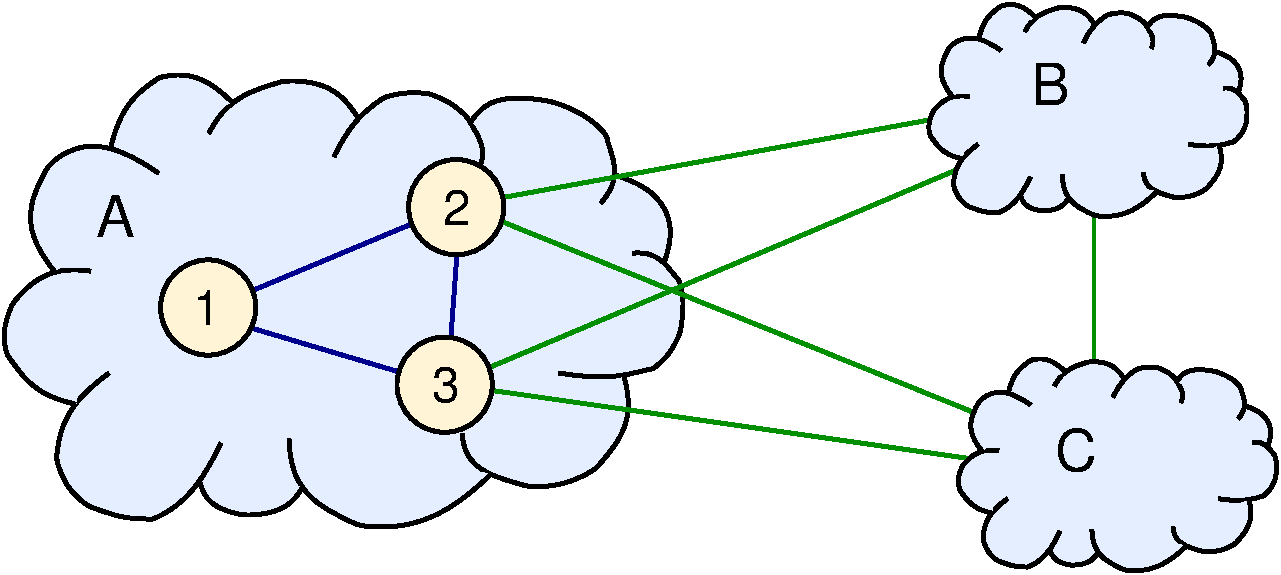
\includegraphics[width=\oneup]{example_grav_2}}
\def\HotPotatoIn		{\centering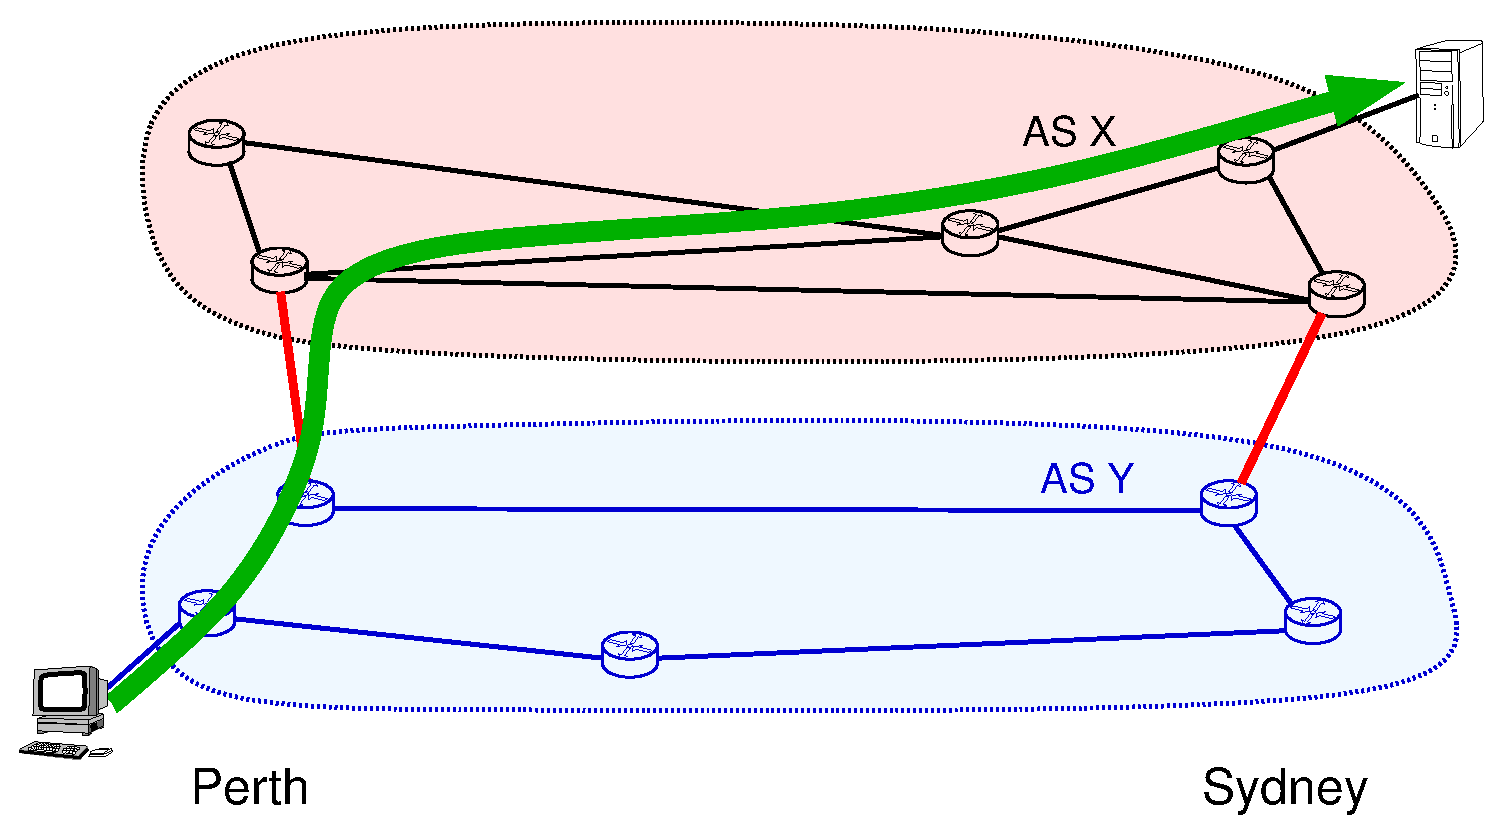
\includegraphics[width=\twoup]{hot_potato}}
\def\HotPotatoOut		{\centering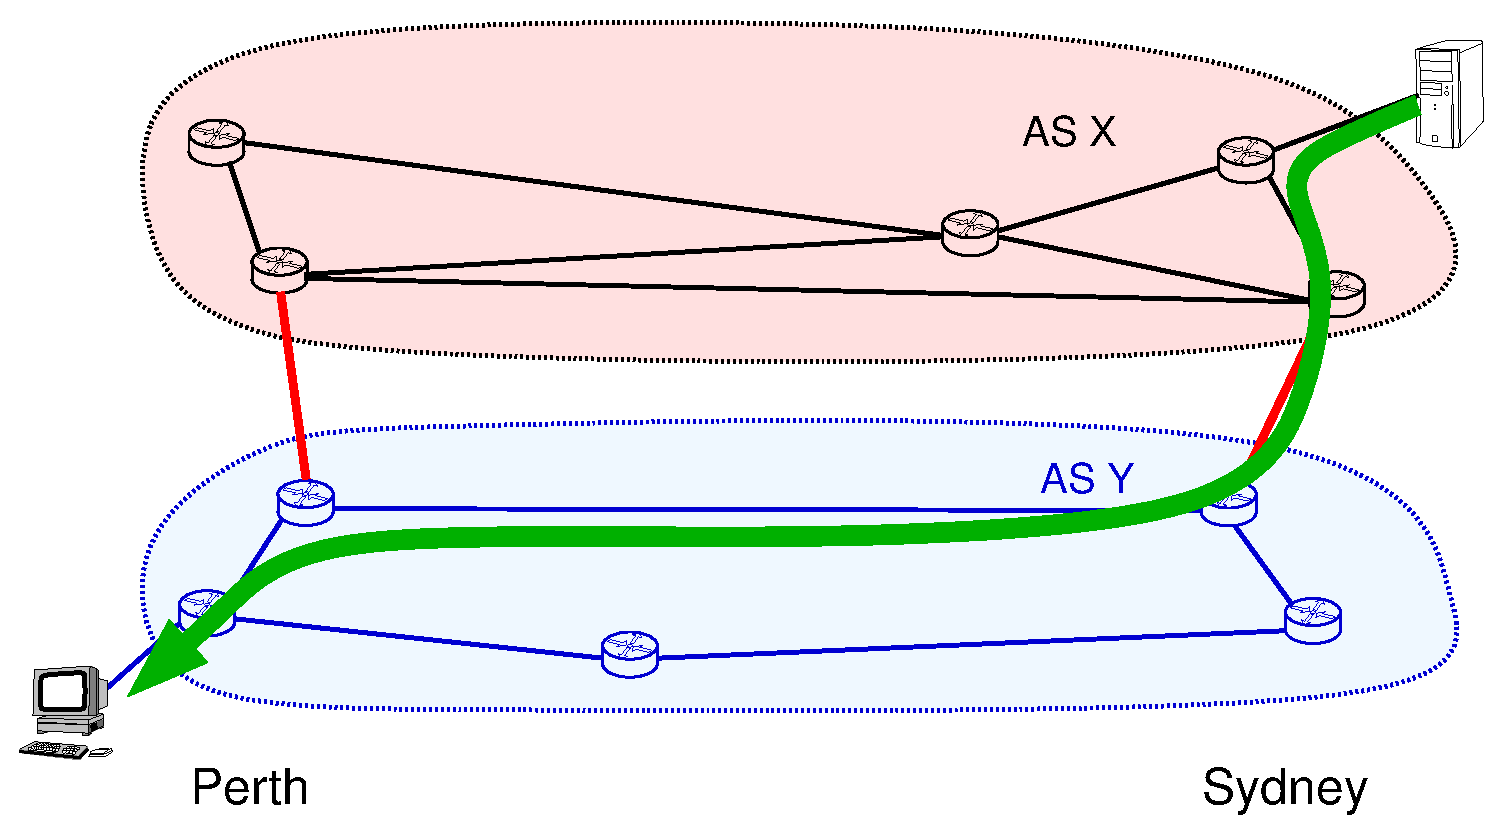
\includegraphics[width=\twoup]{hot_potato_2}}
\def\GravityEx			{\centering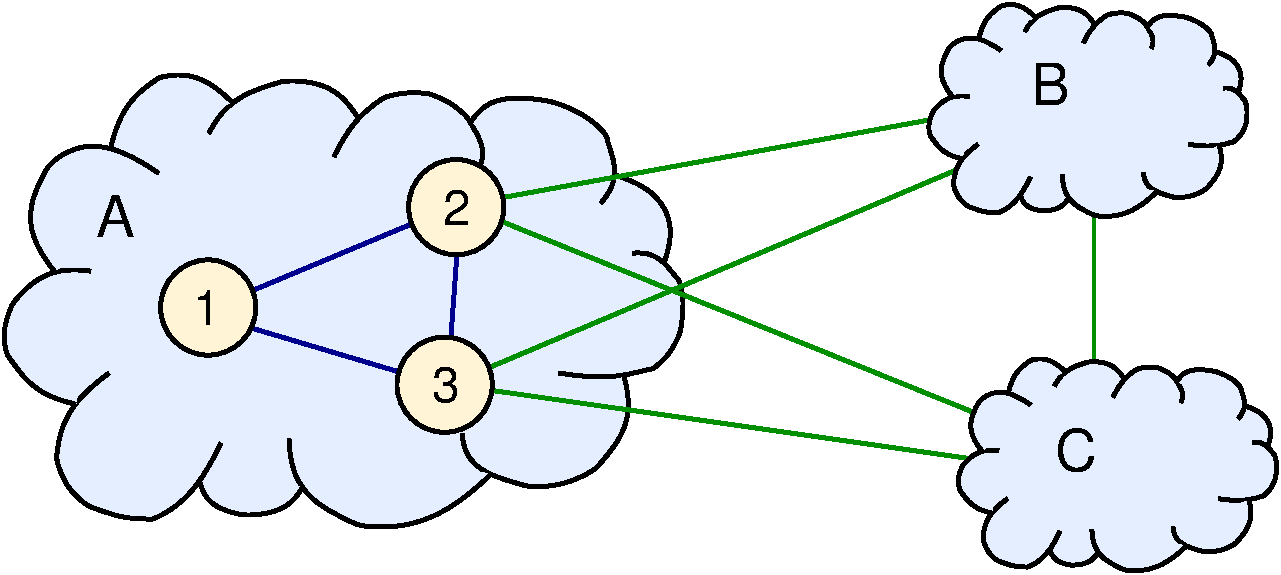
\includegraphics[width=0.7\oneup]{example_grav_2}}
\def\GravityInternal		{\centering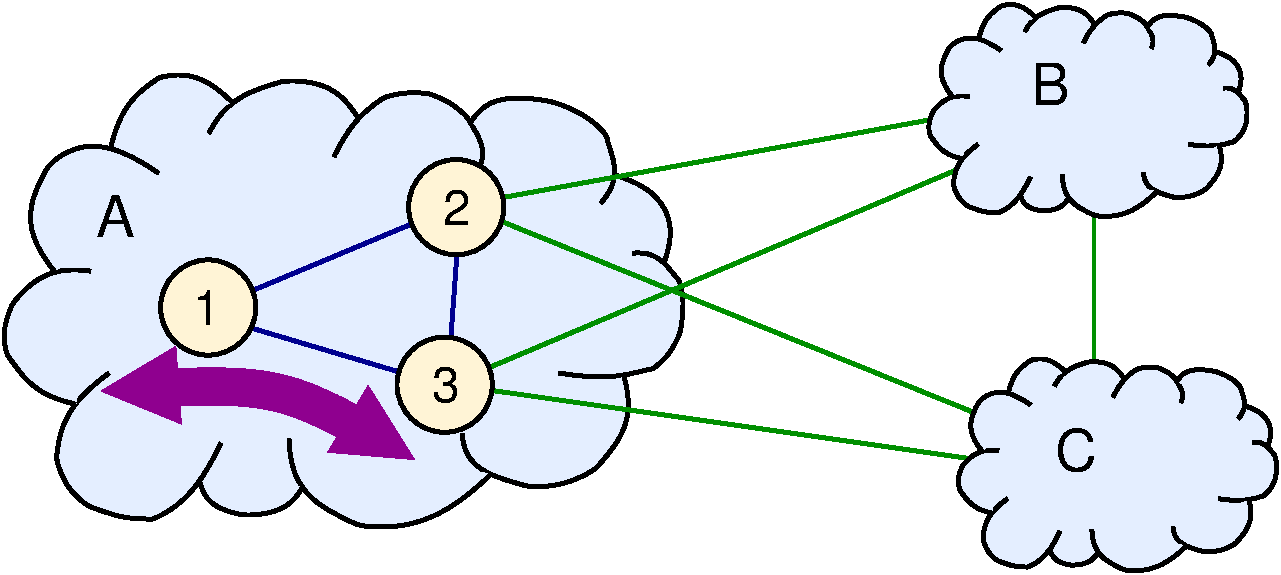
\includegraphics[width=\twoup]{example_grav_int}}
\def\GravityIn			{\centering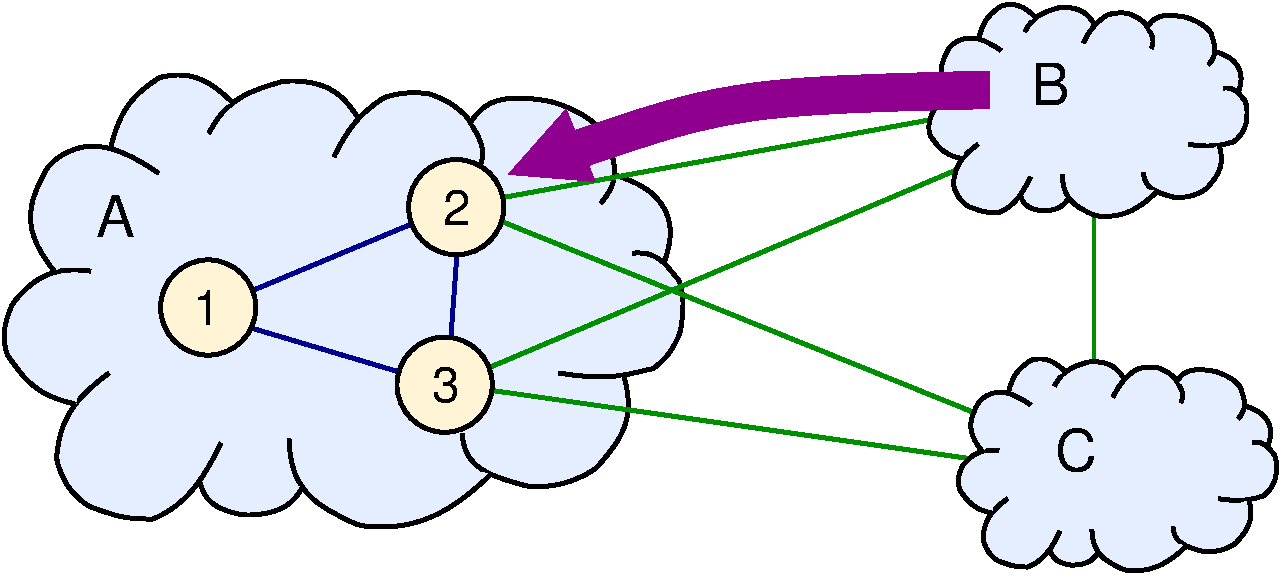
\includegraphics[width=\twoup]{example_grav_in}}
\def\GravityOut			{\centering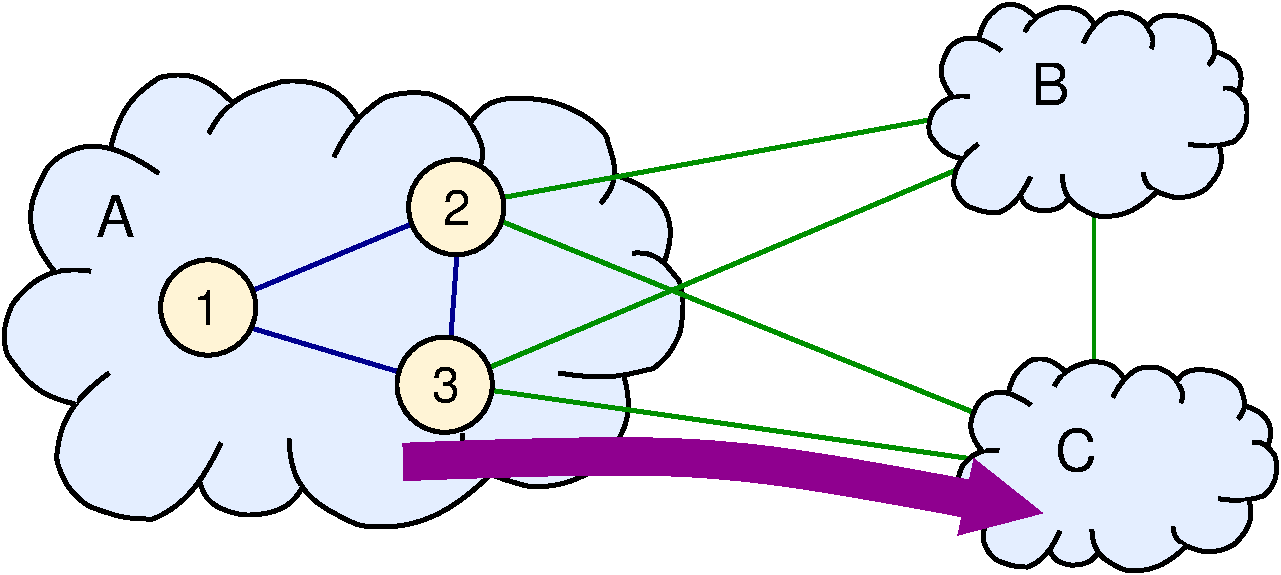
\includegraphics[width=\twoup]{example_grav_out}}
\def\GravityExternal		{\centering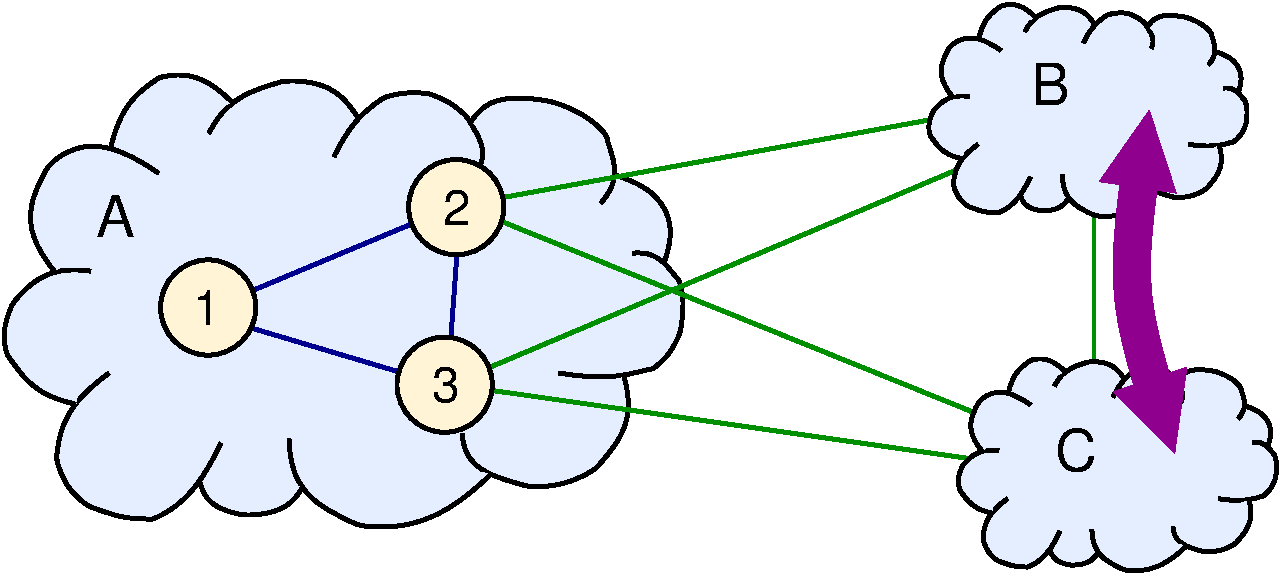
\includegraphics[width=\twoup]{example_grav_ex}}
\def\Topology			{\centering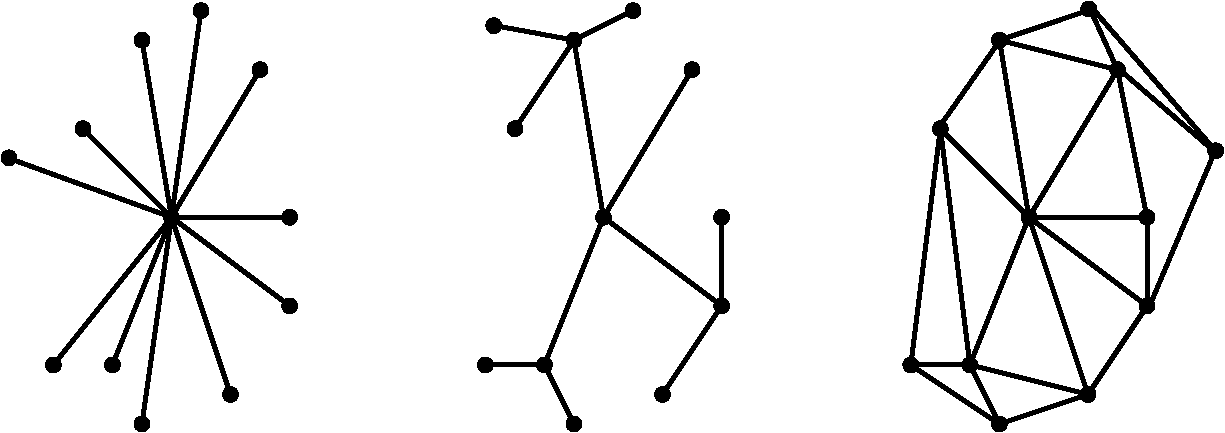
\includegraphics[width=0.9\oneup]{baran}}

%%%%%%%%%%%%%%%%%%%%%%%%%%%%%%%%%%%%%%%%%%%%%%%%%%%%%%%%
\begin{document}

%\begin{titlepage}

\title{Internet Traffic Matrices: A Primer}


\author{
Paul Tune and Matthew Roughan\\
School of Mathematical Sciences\\
The University of Adelaide, Australia.\\
\texttt{\{paul.tune,matthew.roughan\}@adelaide.edu.au}
} 


%\author{Paul~Tune, Matthew~Roughan \thanks{The authors are with the School of Mathematical Sciences, The University 
%of Adelaide, Australia (Email: \{paul.tune,matthew.roughan\}@adelaide.edu.au).}} 
\vfill
\date{}

%\end{titlepage}
\maketitle
\begin{abstract}
  The increasing demand of various services from the Internet has led
  to an exponential growth of Internet traffic in the last decade, and
  that growth is likely to continue. With this demand comes the
  increasing importance of network operations management, planning,
  provisioning and traffic engineering. A key input into these
  processes is the \textit{traffic matrix}, and this is the focus of
  this chapter.

  The traffic matrix represents the volumes of traffic from sources to
  destinations in a network. Here, we first explore the various issues
  involved in measuring and characterising these matrices. The
  insights obtained are used to develop models of the traffic,
  depending on the properties of traffic to be captured: temporal,
  spatial or spatio-temporal properties. The models are then used in
  various applications, such as the recovery of traffic matrices,
  network optimisation and engineering activities, anomaly detection
  and the synthesis of artificial traffic matrices for testing routing
  protocols. We conclude the chapter by summarising open questions in
  Internet traffic matrix research and providing a list resources
  useful for the researcher and practitioner.
\end{abstract}


%\newpage
%\tableofcontents

%\newpage
% Introduction
\section{Introduction}
%
Since the end of the 20th century, wireless networking is experiencing explosive growth, driven by the popularity of wireless telephony on one hand, and by the development of wireless computer networks on the other hand. Both trends are currently merging into a single attempt: enabling massive wireless Internet access. This phenomenon was inspired by Norman Abramson's pioneer work on packet radio networks \cite{ABRAMSON-70} in the 1970s, and made possible by the authorization of wireless spectrum use for civil telecommunication purposes, in the 1980s\footnote{ISM (Industrial, Scientific, Medical) bands, released in 1985 by US Federal Communications Commission (FCC) for unlicensed use.}. At first, this deregulation encouraged the democratization of wireless telephony, in the 1990s, thanks to the availability of cheaper, more efficient hardware stemming from Cold War military industry efforts. Since 2000, the introduction of new wireless communication standards using the spectrum authorized for civil use has also fueled the development of wireless computer networks and wireless Internet access.
%
\subsection{Managed Wireless Networks}
%
Wireless Internet access is nowadays mostly provided via link layer technologies such as Wifi (IEEE 802.11 infrastructure mode standards \cite{IEEE-802-11}), WiMAX\footnote{Worldwide Interoperability for Microwave Access.} (IEEE 802.16 \cite{IEEE-802-16}), UMTS\footnote{Universal Mobile Telecommunications System.} or LTE\footnote{Long Term Evolution.} (3GPP standards \cite{3GPP}), on user terminals such as smartphones, tablets, laptops, {\em etc}. Such technologies have in common a communication model that is similar to the local wired network model: user terminals (hereafter denominated \glslink{host}{\em hosts}) access the Internet through a dedicated, authoritative infrastructure device (hereafter denominated \glslink{router}{\em router}). In that sense user terminals are competing ``consumers" of the same networking resource, which consists locally in access to the \glslink{router}{router} granting internetwork (Internet) connectivity. \glslink{router}{Routers}, on the other hand, are ``providers" of the networking resource, and collaborate with one another to provide this resource, \emph{i.e.} internetwork connectivity. This similarity enables IPv4 and IPv6 protocol suites to run quite naturally over such wireless access networks, although IP protocols were in fact designed for wired networks at a time when massive use of wireless Internet access was not yet envisioned. \ \\ \ \\
%
The basic mechanisms provided by IEEE 802.11 infrastructure mode, WiMAX, UMTS or LTE thus provide communication capabilities over a single wireless hop, between a user terminal and an infrastructure access point. 
Some extensions of these basic mechanisms provide direct device-to-device communication (as the Wifi ad hoc mode) or even multi-hop wireless communication through relays planned in advance ({\em e.g.} with LTE or WiMAX). However, these wireless networks all have in common their \emph{managed} nature: they depend entirely on an infrastructure planned and deployed in advance, controlled by an operator. This chapter does not focus on such networks.

\subsection{Spontaneous Wireless Networks}
\label{ss:spontaneous}
%
Although so far not as successful as managed wireless networking, an alternative type of wireless networks has also emerged since 2000: \emph{spontaneous wireless networks}. Inspired by the Push-To-Talk concept used in walkie-talkies (portable half-duplex radio transceivers developed during the Second World War), spontaneous wireless networks depart from the traditional distinction between \glslink{router}{routers} and \glslink{host}{hosts}, whereby each user terminal (hereafter, {\em node}) may behave as a \glslink{router}{router} and a \glslink{host}{host} simultaneously. In spontaneous wireless networks, user terminals are thus ``prosumers" ({\em i.e.} both producers and consumers) of networking resources instead of mere consumers. Terminals self-organize to provide multi-hop wireless communications among themselves, with or without help/control from infrastructure devices. Each node may thus simultaneously originate/receive traffic (role of a \glslink{host}{host}), as well as forward traffic on behalf of other terminals (role of a \glslink{router}{router}). \ \\ \ \\ 
%
Popular examples of spontaneous wireless networks include mobile ad hoc networks, wireless mesh networks, wireless sensor or actuator networks, wireless smart meter networks, vehicular networks, opportunistic wireless networks or delay tolerant networks. Spontaneous wireless networks are considered as interesting solutions to extend and offload managed wireless networks hampered by increasingly heavy smartphone data communications \cite{NY-TIMES}. They can also increase the resilience of the network in scenarios where infrastructure is not usable, due to a disaster, to the military situation or to the political situation, for instance \cite{COMMOTION}. In addition, spontaneous wireless networking is an effective way to extend the reach of wireless Internet access, without costly additional infrastructure deployment \cite{OLPC}. \ \\ \ \\ 
%
Popular link layer technologies providing device-to-device communication in spontaneous networks include so far IEEE 802.11 ad hoc mode \cite{IEEE-802-11} and IEEE 802.15.4 \cite{IEEE-802-15.4}. However, in order to provide multi-hop communication in spontaneous wireless networks, additional techniques have to be employed on top of such link layer technologies, and that is the subject of this chapter. The focus is put on the use of standard IP protocols to enable multi-hop wireless communications in spontaneous wireless networks -- in order for these networks to effectively blend in the Internet, where appropriate.%\ \\ \ \\
%
\paragraph{Handling heterogeneity at layer 3} Since the early days of computer networking and the first steps of today's Internet, the diversity of networking technologies has been handled exclusively at the physical and the link layers (layers 1 and 2 OSI). The internetworking layer (layer 3) has been conceived as a ``convergence layer" in which a single protocol (the Internet Protocol, IP) runs unchanged on top of heterogeneous interconnected networks, as it can be observed in Figure \ref{f:conv} \cite{miya}.

\begin{figure}[ht]	% H-must be here or [htb]
\centering
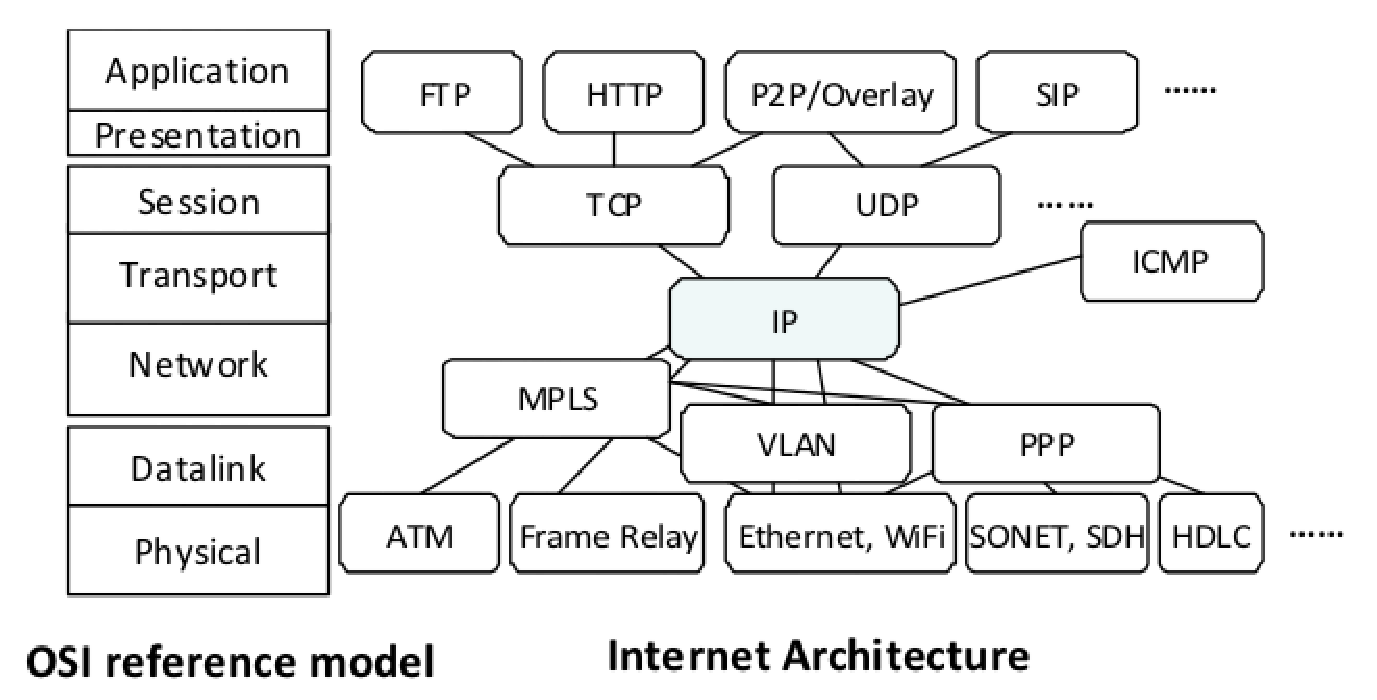
\includegraphics[width=0.7\textwidth]{Figures/protostack-crop.pdf} %	** if .eps or .pdf, don't need extension}
\caption{OSI reference model and IP networking architecture \cite{miya}.}
\label{f:conv}
\end{figure}
%
The development of wireless technology entails however substantial changes in the way that networks are usually represented and conceived. Characteristics of spontaneous wireless networks cannot be handled exclusively at lower layers of communication, as they challenge some of the key assumptions of the IP-based networking architecture. They need thus to be taken into account at layer 3. As more flexible wireless networks are deployed and get increasingly interconnected and integrated with other networks --or in the Internet--, the use of IP over these networks need thus to be adapted or reconsidered. The {\bf first contribution} of the chapter is a review of these considerations, as it elaborates on how the IP-based network architecture is challenged by spontaneous wireless networks.
%
\subsection{Mobile Ad hoc and Low-Power Lossy Networks}
\label{ss:manet_lln}
%
IP protocols are developed, standardized and maintained by the Internet Engineering Task Force (IETF \cite{IETF}). Most of the IETF's protocol design and standardization activities have so far focused on two categories of spontaneous wireless networks: Mobile Ad hoc Networks (MANETs) and Low-Power Lossy Networks (LLNs).

% ({\em e.g.}, a \glslink{router}{router} with multiple \glslink{host}{hosts} and wireless communications devices)--herein simply referred to as `nodes'--

\paragraph{Mobile Ad hoc Networks (MANETs)} According to the IETF's terminology (defined in RFC 2501 \cite{rfc2501}), a MANET consists in a set of ``mobile platforms (..) --herein simply referred to as `nodes'-- (..) which are free to move about arbitrarily. The nodes may be located in or on airplanes, ships, trucks, cars, perhaps even on people or very small devices, and there may be multiple \glslink{host}{hosts} per \glslink{router}{router}. A MANET is an autonomous system of mobile nodes. The system may operate in isolation, or may have gateways to and interface with a fixed network" \cite{rfc2501}. Note that this definition {\em allows} \glslink{router}{router} mobility, but it is {\em not restricted} to mobile networks; the term includes all wireless multi-hop ad hoc networks, regardless of whether they are static or not. 

\paragraph{Low-Power Lossy Networks (LLNs)} According to the IETF's terminology (defined in {\tt draft-ietf-roll-terminology-12}\footnote{An Internet-Draft in the Last Call for becoming an RFC, at the the time of writing this chapter.} \cite{draft_lln}), LLNs are ``typically composed of many embedded devices with limited power, memory, and processing resources interconnected by a variety of links, such as IEEE 802.15.4, LowPower WiFi" \cite{draft_lln}. LLNs are thus a more specific case of MANETs (as defined in the previous paragraph), in which \glslink{router}{routers} typically operate with constraints on processing power, memory, and energy (battery power). Their interconnections are characterized by high loss rates, low data rates, and link instability.  LLNs are comprised of anything from a few dozen to thousands of \glslink{router}{routers}.  Supported traffic flows include point-to-point (between devices inside the LLN), point-to-multipoint (from a central control point to a subset of devices inside the LLN), and multipoint-to-point (from devices inside the LLN towards a central control point). Alternative, but similar terminology is employed in {\tt draft-ietf-lwig-terminology} \cite{bormann13}, which defines the terms ``constrained nodes" and ``constrained networks" with various classes of constraints. \\

Concrete examples of MANETs and LLNs include the following three use cases, selected only for illustrative purposes, to hint at the wide heterogeneity of features, requirements and user expectations that one must address in spontaneous wireless networking.

\paragraph{Vehicular Ad hoc Networks (VANETs)} Communication in VANETs is enabled between moving vehicles in urban scenarios or roadways, (possibly) with fixed devices installed in Roadside Units (RSUs) along the road/street. The combination of vehicles and RSUs forms a mobile, highly dynamic ad hoc network. Devices participating in vehicular networks (either inside vehicles or in RSUs) have neither significant energy constraints nor severe computational limitations, but those installed in vehicles are not, in general, cooperative and willing to dedicate resources to others' communication. Research in these networks has typically focused on safety applications, such as distribution along the highway of information about traffic-related events -- \emph{e.g.}, jams or accidents \cite{bc_vanet}. Other purposes could be also considered, such as dissemination of service availability along the highway (gas stations, tolls, accommodation, etc.). As such, a VANET is a category of MANET.

\paragraph{Community Wireless Mesh Networks} These are cooperative, non-commercial networking projects in which users join and contribute to the deployment of the network, in particular by sharing resources and allowing the use of their devices as networking relays. Several initiatives have flourished in the last years, such as Spain's {\em Guifi} \cite{GUIFI}, mostly deployed over the Eastern coast of Spain (Catalonia and Valencia) but also present in many other parts of the country. Other examples include Germany's {\em Freifunk} \cite{FREIFUNK} and Austria's {\em Funkfeuer} \cite{FUNKFEUER}. Some of them cover large geographical areas and contain thousands of nodes\footnote{{\em Guifi.net}, for instance, claims 31865 nodes, 20425 of them being ``operating nodes" (last query to {\tt http://www.guifi.net} on April 10th, 2013).}. These networks are typically static, most of the links are wireless links operating in free (unlicensed) frequency bands. Their topology and capacity evolve dynamically, in an unplanned manner, subject to events such as the ingress and egress of users, the subsequent availability of new links and resources or the upgrade of a particular networking region. These networks enable free communication among their users, but they can also provide access to the Internet if there are gateways available. As such, a community wireless mesh networks is also a category of MANET.

\paragraph{Wireless Sensor Networks (WSNs)} WSNs are collections of sensors intended to measure one or several properties of the environment in which they are deployed. Communication facilities required by such networks need to include, at least, the transmission of collected information from the sensors to a gateway or central server that stores and eventually process it, and the transmission of information (\emph{e.g.}, configuration instructions or measurement schedules) from the server to one or more sensors. There is a broad range of information that may be collected and exchanged through WSNs, some examples including climate studies, bird observation, power monitoring in buildings or tracking of patients' health parameters with body sensors. Properties of a WSN may vary depending on the purposes of the sensor deployment, but there are some usual constraints. Sensors are often battery driven, the lifetime of the sensor is limited by the battery lifetime. Protocols for enabling communication within WSNs must therefore be designed with energy consumption and energy-efficiency in mind. As such, a wireless sensor network is a category of LLN.\\

Despite their heterogeneity, these use cases -- and other applications of spontaneous wireless networks -- have common characteristics, including bandwidth scarcity and need for self-organization. These characteristics both require the use of efficient, highly decentralized routing and flooding mechanisms, able to react quickly to topology changes without overloading the network. This chapter thus focuses more specifically  on IP protocols that enable routing and flooding in MANETs and LLNs. While plenty of protocols have been proposed in the literature, only few have been effectively implemented, standardized and used in real-world deployments. The {\bf second contribution} of the chapter consists in:

\begin{enumerate}[(1)] 
\item an analysis of the main implications of wireless mesh characteristics on the task of flooding and routing typically implemented in upper-layer protocols; and 
\item a description and discussion of the key mechanisms and operation of the main protocols deployed so far and standardized at the IETF for routing in MANETs, in LLNs and in heterogeneous wired/wireless inter-networks.
\end{enumerate}

\subsection{Reader's Guide}

Reader is assumed to be familiar with the main concepts of computer networking and the TCP/IP network reference model, whose terminology is used in this chapter. Interested readers are referred to the book of Tanenbaum {\em et al.} \cite{tanenbaum} for details; the glossary at the end of the chapter displays standard definitions of the basic networking concepts. Basic knowledge of the Internet Protocol (IP) operation, addressing model, routing and Internet architecture is also preferable, but not necessary. These elements are briefly overviewed in section \ref{s:fundamentals}, in order to better highlight the issues that arise with the traditional IP model in spontaneous wireless networks, addressed in section \ref{s:comm_wless}. This section describes the conditions under which wireless communication occurs, and examines their impact on the communication performance and the architecture of spontaneous wireless networks. In particular, the section explains the non-suitability of the conventional IP networking model for spontaneous wireless networks, and discusses an alternative model. \ \\ \ \\ 
%
The rest of the chapter focuses on the mechanisms and protocols that have been designed to handle flooding and routing in spontaneous wireless networks, paying a particular attention to the efforts deployed at the IETF. Section \ref{s:flood_rtg} motivates and presents the mechanisms, and section \ref{s:specific} describes the routing and flooding protocols that have been specifically designed in the IETF to operate on MANETs and LLNs. Section \ref{s:wospf} focuses on the problem of extending legacy Internet routing protocols so that they can efficiently operate on hybrid (wired/wireless) inter-networks. Finally, section \ref{sec:conclusion} concludes the chapter.


% Traffic Matrices

\clearpage
\section{Definitions and Notation}
\label{sec:tm}

In this section, a formal approach to networks and traffic matrices is
defined.  Traffic originates from a \emph{source} and is delivered to
a \emph{destination} (or several destinations). The traffic traverses
a set of \emph{links} between some set of sources and destinations.
The links connecting these define the \emph{topology} of the network,
and the paths chosen by traffic flows determine the {\em
  routing}. Traffic may be split across multiple paths by load
balancing, or may keep to a single path.  Often, sources and
destinations are identified with network devices such as switches or
routers, but they can also refer to a location in a logical space
attached to the network, for instance IP addresses of prefix blocks.

Let $\Omega$ denote the non-empty set of all sources and destinations
in a network and let $|\Omega| = N$.  The sources and destinations
often have a physical, geographic location, and so we regard their
indices as {\em spatial variables}, even when they are actually
logical entities, such as Autonomous Systems (ASes), or cannot be
directly identified as network devices, as with IP addresses.

\begin{figure}
  \begin{center}
    \begin{minipage}[m]{0.64\columnwidth}
      \vspace{0pt}
      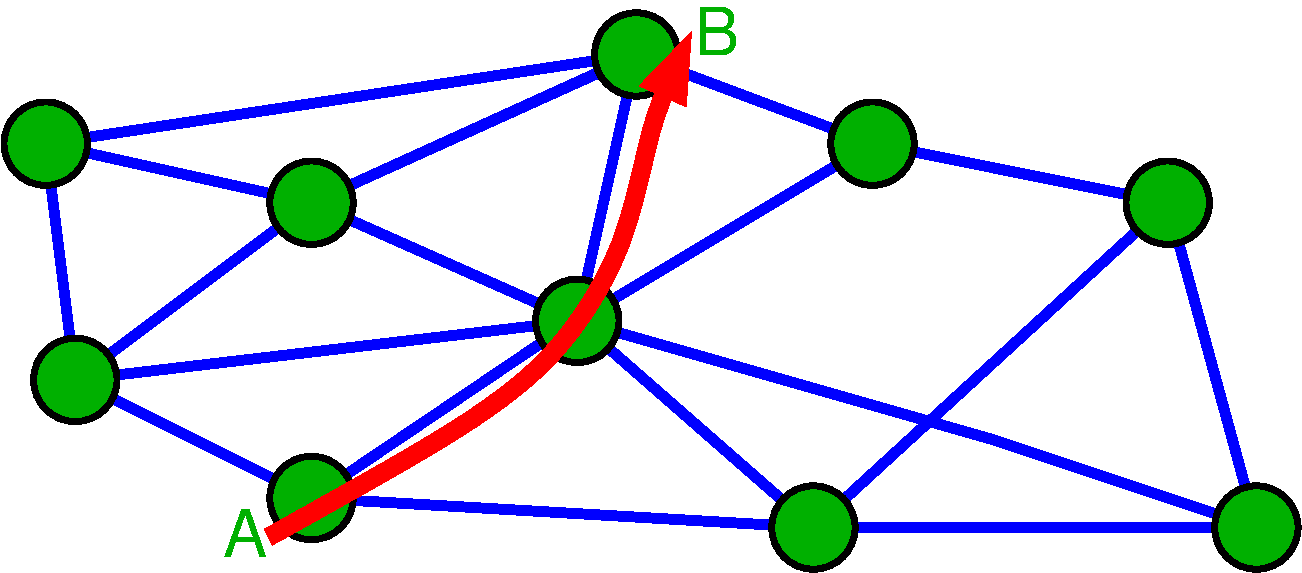
\includegraphics[width=0.9\columnwidth]{traffic_matrices.pdf}      
    \end{minipage}
    \hspace{-10mm}
    \begin{minipage}[m]{0.3\columnwidth}
      \vspace{0pt}
      $$ X = \displaystyle
              \left( \begin{array}{lllll}
                x_{AA} & {\color{red} x_{AB}} & x_{AC} & \cdots \\
                x_{BA} & x_{BB} & x_{BC} & \cdots \\
                \vdots & \vdots & \vdots & \ddots \\
	      \end{array} \right)
    $$
  \end{minipage}
  \caption{An example of a traffic matrix. Note that often the
    diagonal elements, $x_{AA}, x_{BB}, \ldots$ are zero as this
    traffic does not cross the network, however, in almost as many
    cases it is non-zero because a ``node'' in the graph represents an
    aggregation of devices such as a PoP or an AS. In these cases we
    often do wish to measure these diagonals, even though they may not
    cross the logical links pictured, because they affect traffic
    engineering within the PoP, for example.
  \label{fig:tm} }
  \end{center}
\end{figure}


A traffic matrix is naturally represented by a three dimensional,
nonnegative hyper-matrix $\bX(t)$, with $i,j$-th entry $X_{i,j}(t)$.
Each entry represents the traffic volume, or demand, measured in terms
of bytes or packets, from source $i$ to destination $j$ in time
interval $\lbrack t, t+\Delta t) \subset \cT$, the full measurement
interval being denoted by $\cT$. As an aside, a matrix representation is
useful for the representation of other aspects of the network, for
instance, delay, jitter, loss, bottleneck-bandwidth and distance
\cite{Medina02Taxonomy}, but throughout the chapter, traffic will be
the focus. Whenever the context is clear, for example, when
considering only the spatial structure of the matrix, the time index
$t$ is dropped. An abstract example of the traffic matrix is presented
in \autoref{fig:tm}.

A closely related concept is the {\em demand matrix}, distinct from
the traffic matrix because the former is {\em offered load}, and the
latter {\em carried load} \cite{Feldmann01TMdemand}. 
They may be the same, but may differ where
congestion limits the carried traffic, or rate limiting is used on
some traffic streams. In general we cannot measure offered traffic,
only carried traffic, and so almost all empirical research has
concentrated on traffic matrices, but it is important to note that
many of the assumptions of traffic matrix models are actually
motivated by intuition about demand matrices, and these may not apply
where the two differ substantially\footnote{Many works make no
  distinction between demand and traffic matrices, leading to
  confusion. Here, we shall try to keep the two distinct: when we say
  traffic matrix, we are referring to carried traffic.}.


% The spatial variable $i$ and $j$
% are generally associated with the address structure of the Internet,
% such as Internet Protocol (IP) addresses, or prefixes of these
% addresses.

Large-scale, real-time monitoring of traffic is intractable at
present, thus limiting measurements to the average traffic in a
discrete time interval. Shorter time intervals \ie~small $\Delta t$,
benefit anomaly detection applications, the tradeoff being a
possibility of uncertainty from traffic burstiness at shorter time
scales combined with larger potential measurement or sampling
errors\footnote{Traffic is typically sampled at the backbone network
  level to cope with the tremendous volumes of data that could be
  collected.}. Longer time intervals result in ``smoother'' traffic, 
  averaging out measurement errors. However, this smooths out
real variability in the traffic as well, and can result in meaningless
estimates in the presence of strong non-stationarity. Hence, the
choice of $\Delta t$ depends on the application and available
measurements. Common choices range from 5 minutes to an hour. Further
discussion on the temporal properties of traffic flows is found in
\autoref{sec:models}.

There are two popular definitions of traffic matrices: the
origin--destination (OD) matrix and the ingress--egress (IE) matrix.
\begin{enumerate}

\item \textbf{OD traffic matrix}: this matrix measures traffic from
  true source to destination, \ie~the point that generates a packet
  to the point that receives it. In the Internet, it is perhaps most
  reasonably defined in terms of Internet Protocol (IP) addresses.
  However, if $\Omega$ is defined over the entire IPv4 address space of
  $2^{32}$ addresses (with even more for IPv6), this poses storage and
  computational problems. Moreover, the matrix would be very
  sparse. What's more, protocols such as NAT, HTTP proxies and
  firewalls may obscure the true IP address mappings. One way to
  overcome some of these deficiencies is to aggregate the traffic
  matrix into blocks of IP addresses, frequently using routing
  prefixes. Bharti \etal \cite{Bharti10Invisible} defined the idea of 
  \textit{atomic aggregation}
  to partially circumvent the problem of size of an OD matrix. 
  If the logical indexing chosen is \textit{atomic}, then a 
  non-zero element of an OD traffic matrix implies that all 
  flows between the particular source and destination 
  pair is fully visible to the network operator (see \cite{Bharti10Invisible}
  for details).	

\item \textbf{IE traffic matrix}: any single network operator sees
  only a small proportion of the Internet OD matrix. Thus this matrix
  is not just unknown, but unmeasurable (by a single
  operator). Instead, many operators find that using their edge
  routers (or even the edge links) as sources and destinations results
  in a local traffic matrix of great use. We call this the IE traffic
  matrix as the set $\Omega$ includes ingress, \ie~traffic going into
  the network, and egress, \ie~traffic flowing out of the network,
  points as proxies for sources and destinations. A single ingress or
  egress ``node'' may denote a router, a collection of physically
  co-located routers called a Point of Presence (PoP), or some other
  abstract collection of traffic ingress/egress points depending on
  the level of coarseness required in the modelling process. The PoP
  level convention is often adopted as it provides a simple
  visualisation of the network its operators.
\end{enumerate}

IE traffic matrices can be obtained in a number of ways. They can be
formed from OD traffic matrices simply by mapping IP prefixes to
ingress/egress locations in the network, but this assumes knowledge of
all flows traversing the ingress/egress nodes.  Traffic at egress
nodes may be inferred from router data (see the next section) and
measurements of ingress traffic, but typically, the converse is
difficult. Likewise, it is usually difficult to form an OD matrix from
IE matrices.

Consequently, the IE traffic matrix is frequently adopted for network
optimisation applications as it is more practical to measure, and
because in aggregating traffic the OD flows are ``bundled'' together
into locally meaningful groupings. A network may carry flows between
billions of IP address pairs and millions of prefix pairs, but only
thousands of router pairs, and hundreds of PoP pairs.  In this way,
the IE matrix is a more compact representation, but more importantly,
the aggregation of the traffic into large bundles results in a
smoothing effect on the data, reducing the number of independent
parameters that may have to be estimated. At the PoP level, the
aggregation of flows results in averaging out sampling error (similar
to the choice of $\Delta t$ above). This is highly beneficial for
numerical iterative algorithms used to estimate the traffic matrices,
as aggregation leads to better conditioning of the traffic matrix. The
trade-off, unfortunately, is the loss of fine grained data, as one can
no longer observe IP-level flow data, or examine application profiles.

Another consideration worthy of concern in applying traffic matrices
is {\em invariance}.  A good representation of the traffic has
to be invariant to other network aspects, such as routing and the
network topology. For instance, if the traffic matrix for a network
changes in response to changes in link placement, then the matrix is
not terribly useful for network design. IE matrices are subject, for
example, to large changes due to routing shifts, and this means that
they are less useful to operators compared to OD matrices. However,
the practicalities of measurements mean that IE matrices may be all
that is measurable.

% That leads naturally to our next topic: measurement of traffic
% matrices. 

% Another example was discussed in \cite{Alderson06Topology} using the G\'{E}ANT \cite{GEANT} network for illustration, where a 
% regional network uses the G\'{E}ANT router to transit traffic within the regional network itself. The result is a net increase of the traffic 
% demands at the nodes being used for this purpose, although these demands themselves do not traverse G\'{E}ANT. Also, distortions 
% may occur in the form of hot potato routing \cite{Paxson97Routing}; see Section \ref{sec:models}. Despite 
% these issues, due to the practicality of the IE traffic matrix, focus will generally be on the IE traffic matrix, unless specified otherwise.



\subsection{Example}

As an example we present the Abilene (Internet2) data from 2004 that
was used in several studies
\cite{Zhang05Anomography,Roughan05GravSynth,Alderson06Topology}.  The
backbone network is located in North America (see
\autoref{fig:abilene_2004_map}).  The traffic data contains averages
over 5 minute intervals, from March 1st to September 11th, 2004
(though there are some missing periods).  The dataset is an
Ingress-Egress, router-router\footnote{In Abilene, at the time, the
  routers almost corresponded to PoPs.} traffic
matrix. \autoref{tab:traffic_matrix} shows one example traffic matrix
from that period, along with row and column sums.

% created by TrafficMatrix::latex_write
% source = Abilene/Internet 2 network
% time interval = 5 minutes
% topology = 
% time = 16-25-00
% date = 2004-04-15
% name = Abilene, 2004
% sampling = 1 in 100 packets
% additional information = as measured using netflow
% created by = TrafficMatrix::write, version 1
% type = ingress/egress, router/pop-level, traffic matrix
% cite = Network Anomography, Yin Zhang, Zihui Ge, Albert Greenberg, Matthew Roughan, ACM/Usenix Internet Measurement Conference, Berkeley, CA, USA, 2005.
% creation date = Mon Jun 24 15:21:43 CST 2013
% units = Gbytes / second
\begin{sidewaystable}[htp]
  \centering
%  \footnotesize
  \begin{tabular}[htp]{r|rrrrrrrrrrrr|r}
          & \multicolumn{12}{c|}{Destination} & \\
      Source &   1 &   2 &   3 &   4 &   5 &   6 &   7 &   8 &   9 & 10 &  11 &  12 & Row sum \\
    \hline
   1 &    0.07 &     0.07 &     0.43 &     0.00 &     0.06 &     0.12 &     0.06 &     0.00 &     0.05 &     0.00 &     0.00 &     0.25 &     1.12 \\
   2 &    0.00 &     4.09 &     6.42 &     0.06 &     7.07 &     4.42 &     1.59 &     0.02 &     3.24 &     0.03 &     0.16 &    11.09 &    38.18 \\
   3 &    0.00 &     4.70 &    25.48 &     4.11 &    13.99 &    11.53 &     3.31 &    87.27 &     5.22 &     0.01 &     0.08 &     7.70 &   163.38 \\
   4 &    0.00 &     1.93 &    10.25 &     1.68 &     5.63 &     6.11 &     2.59 &     0.01 &     4.11 &     2.60 &     0.04 &     5.92 &    40.88 \\
   5 &    0.00 &     4.76 &     0.25 &     0.01 &    24.06 &     0.04 &     0.01 &     0.02 &     1.24 &     0.02 &     0.03 &    18.05 &    48.49 \\
   6 &    0.00 &     2.87 &    23.73 &     1.55 &    13.53 &     4.78 &     2.89 &     0.01 &     9.45 &     0.08 &     0.50 &     7.64 &    67.02 \\
   7 &    0.00 &     0.67 &     4.79 &     1.92 &     3.50 &     2.24 &     1.25 &     0.00 &     0.93 &     0.02 &     0.03 &     3.31 &    18.67 \\
   8 &    0.00 &     4.18 &     2.58 &     5.80 &    26.35 &     0.17 &     0.16 &     1.41 &    10.88 &     2.11 &     3.64 &    16.67 &    73.97 \\
   9 &    0.00 &     8.61 &    12.34 &     5.71 &    18.21 &    11.05 &     3.84 &     0.41 &    36.36 &     0.02 &     0.52 &    17.31 &   114.37 \\
  10 &    0.00 &     0.18 &     0.04 &     1.71 &     1.69 &     0.00 &     0.06 &     5.61 &     0.96 &     1.82 &     8.44 &     0.36 &    20.86 \\
  11 &    0.00 &     3.47 &     3.28 &     0.54 &     8.60 &     0.13 &     0.93 &     3.92 &     1.77 &     0.81 &     0.61 &     2.32 &    26.38 \\
  12 &    0.00 &    18.20 &    16.04 &     0.83 &    34.03 &    11.18 &     5.64 &     0.09 &    25.57 &     0.08 &     0.80 &    47.02 &   159.47 \\
    \hline
      Column sum &    0.07 &    53.74 &   105.61 &    23.94 &   156.73 &    51.76 &    22.34 &    98.77 &    99.77 &     7.59 &    14.84 &   137.65 &   772.80 \\
  \end{tabular}
 \caption{An Abilene 5 minute traffic matrix from April 15th, 2004 from 16:25--16:30, in Mbps.}
  \label{tab:traffic_matrix}
\end{sidewaystable}


We can immediately see that the matrix is not symmetric, and that
there are quite a range of values. Also notable, the diagonals are not
zero, as there is some measured traffic that enters Abilene, and then
exits at the same PoP.

A timeseries view of the data is seen in 
\autoref{fig:abilene_2004}. The top figure shows the total traffic
during each time interval for the whole dataset, and the bottom figure
shows the first two weeks of the data, overlaid so as to illustrate
the cyclic nature of the data. We can clearly pick out peak traffic
hours, and weekdays from the weekend. However, the variation between
peak and off-peak loads is perhaps smaller than is typical in
commercial environments. 

\begin{figure}[thbp] 
  \begin{center}

    \begin{subfigure}[b]{\oneup}
      \centering
      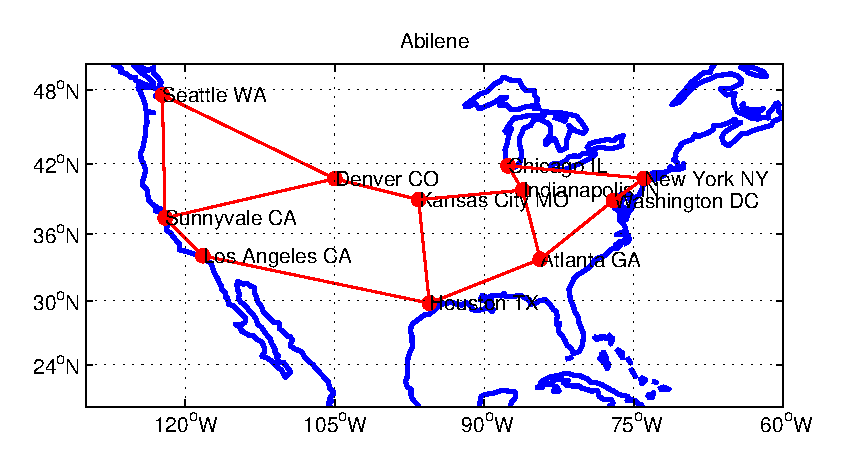
\includegraphics[width=\textwidth]{abilene_map.eps}
      \vspace{-5mm}
      \caption{Map of Abilene PoPs. \autoref{tab:traffic_matrix} is a
        router to router traffic matrix, but there is one router per
        PoP except in Atlanta, where there is a second router. The
        router numbers in the table are alphabetical.}
      \label{fig:abilene_2004_map}
    \end{subfigure}

    \vspace{3mm}
    \begin{subfigure}[b]{\oneup}
      \centering
      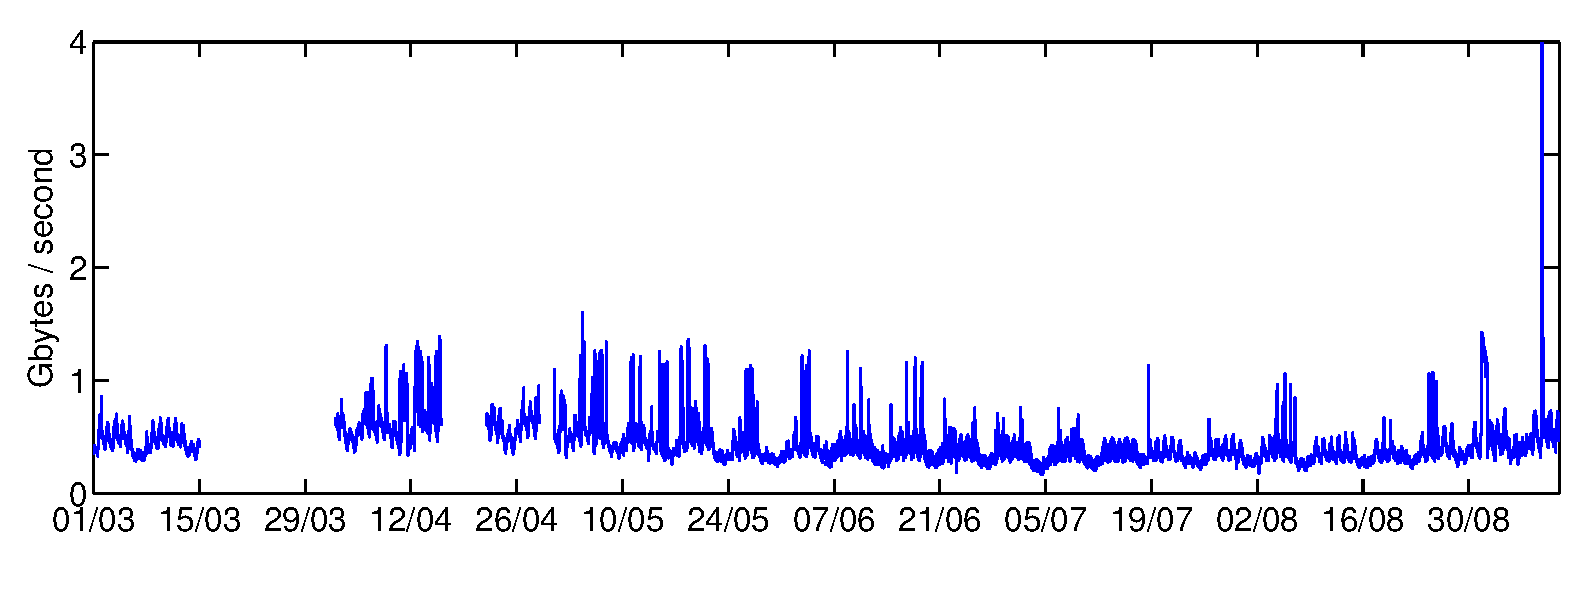
\includegraphics[width=\textwidth]{Abilene_2004_totals.eps}
      \vspace{-9mm}
      \caption{Abilene 5 minute totals of the traffic matrix from
        March 1st to September 11th, 2004.}
      \label{fig:abilene_2004_a}
    \end{subfigure}

    \vspace{3mm}
    \begin{subfigure}[b]{\oneup}
      \centering
      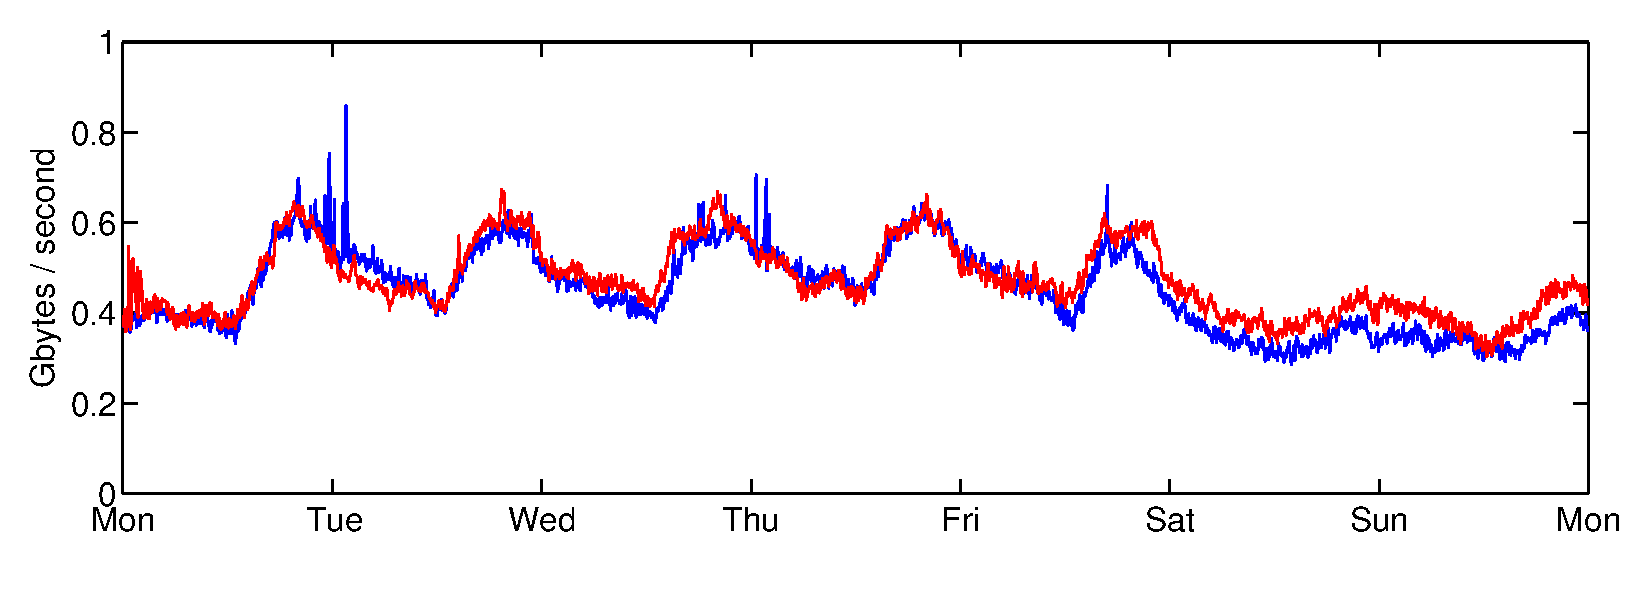
\includegraphics[width=\textwidth]{Abilene_2004_totals_short.eps}
      \vspace{-8mm}
      \caption{The weeks starting March 1st (blue), and March 8th (red).}
      \label{fig:abilene_2004_b} 
    \end{subfigure}  
       
    \vspace{2mm}
    \caption{Abilene, 2004\label{fig:abilene_2004}}
  \end{center}
\end{figure}         

We have endeavoured to put this data into an easily read format, and
placed it onto a web server at 
\url{http://www.maths.adelaide.edu.au/matthew.roughan/traffic_matrices.html},
where we will also place other TM datasets as far as possible, for
comparison studies, or as test datasets for education.

The data illustrates a number of properties of the data, perhaps most notably
the fact that many datasets have anomalous ``spikes'' (these are often
real, but may also be artefacts in the data), and periods of missing
data. The question of how these arise then naturally leads to our next
chapter on measuring traffic matrices. 
  

% Measurement
\clearpage
\section{Measurements}
\label{sec:measurements}

In theory, it is possible to collect accurate data of Internet traffic
from a network. In reality, however, many issues confound such
measurements. Budget constraints driven by the cost of collection, or
the massive data storage facilities required due to the sheer amount
of data traversing a backbone network limit what can be achieved. And
even good measurement systems can suffer from errors and missing
data. Added to this, current operator practice rarely includes any
significant calibration of measurement apparatus, so often the degree
of accuracy of the measurements is unknown.

There are several well-known strategies for collecting traffic
measurements. A {\em packet trace} is a collection of packets headers
(perhaps with some payload) and timestamps.  A packet trace can be
collected through various means, for example, through hardware such as
a splitter placed strategically in optical fibre; adding a monitor
port on a router; or through software tools such as \texttt{tcpdump}
executed on several hosts in a shared network. An OD traffic matrix
can be constructed from such a trace by simple consideration of the IP
address in the packet headers (with the caveats mentioned earlier).

Such an approach is ideal in many respects: we have almost complete
information, and the matrices may be drawn at almost any time
resolution. However, collecting packet traces is expensive due to the
need for dedicated hardware, and the huge amount of storage required:
potentially, over a terabyte of data per hour on OC48 links (2.5 Gbps)
is needed. It is rare for any but the smallest network to be able to
completely instrument its network at this level of detail.

Fortunately, constructing a traffic matrix does not require such
detailed information. Perhaps the most common alternative is {\em
  flow-level aggregation} where packets are aggregated according to a
common flow key.  One popular definition of the key is the 5-tuple
comprised of the IP source and destination address, TCP/UDP source and
destination port numbers and protocol number. A series of packets
possessing a common key is called a \emph{flow}, and we maintain
simple statistics (byte and packet counters, and start and stop times)
for each flow. The aggregation of packets into flows reduces the
number of records needed to be stored by removing redundancies of data
from a packet trace. Flow-level collection is generally performed in
15 minute time bins\footnote{The issue of timing of flows is actually
  somewhat more complicated, but readers should refer to detailed
  descriptions of specific flow-capture protocols for information on
  their particular flow capture.} and is often an in-built function of
a router. The only additional infrastructure required is the Network
Management Station (NMS) and flow records themselves are usually
compressed by the router before being exported to the NMS. Despite
this reduction, flows arrive at a router at rapid rates and the
formation and storage of flow records at a router often burdens the
router's CPU.

To further reduce the number of flow records at a router, sampling
methods are employed. The most popular sampling method is packet
sampling, where incoming packets are sampled based on predetermined
sampling patterns, used, for instance by Cisco's NetFlow
\cite{NetFlow}. Such pseudo-random patterns have a similar effect to
independently picking incoming packets given sufficient mixing of
traffic.  The sampling rates can be adjusted depending on the capacity
of the incoming links with recommendations such as 1 in 256 packets
for OC192 links (10 Gbps). Higher capacity links require aggressive
data reduction, and so lower sampling rates are used.

Packet sampling reduces the number of flows significantly by omitting
many, but it is important to realise that although it may select
\emph{packets} in an unbiased way, it is not unbiased with respect to
\emph{flows}. Packet sampling has a strong bias towards long flows,
since it is more likely to have sampled packets from a long flow than
a short one. Furthermore, the sampled flow size is not the true size
of the flow and there are several works
\cite{Duffield05Sampled,Duffield05Smart} proposing methods to sample
and estimate the true size of a sampled flow. While the strong bias
may be a problem for some applications, there is usually no problem in
using sampled flows to form the IE traffic matrix.

In addition to packet sampling, we may also sample a set of flows, and
these sampled flows can then be used to create traffic matrices. The
resulting reduction in intermediate storage and processing can be
substantial, particularly if the sampling is done in a clever way
\cite{Duffield05Sampled,Duffield05Smart}.

It must be remembered that sampling is an inherently lossy process,
regardless of the underlying sampling method used.  The loss of
information translates into errors or noise in the data. The size of
these errors should, in best practice, be estimated for a given setup,
but most operators do not undertake such procedures due to the
difficulties involved in obtaining ground-truth data with which to
compare to the sampled data. In many cases it is simply assumed that
these errors, once the data is aggregated further into traffic
matrices, are negligible, but this assumption is rarely validated.

Furthermore, there is the problem of possible multiple counting of 
traffic flows from the aggregated records of flows. The problem 
arises if the aggregated flow records come from internal backbone
routers of the network, since a single flow may be recorded more than
once by several routers if it traverses several links. One way to
get around this relies on the placement of the measurement
points. One simply performs traffic measurements at the ingress points.
Specifically, the measurements are performed on the backbone routers 
connected to the access routers, or on dedicated devices placed at the 
links connecting the access routers to the backbone routers. 
In this way, the total incoming traffic of the network may be reliably
measured from the flow records. There is then no longer a problem of 
multiple counting of flows.

Trajectory sampling \cite{Duffield01Trajectory,Duffield04Unreliable} 
is another method. It exploits the pseudorandomness 
of a hash function to simulate random sampling of packets. However, if a flow 
was sampled at one router, it will be consistently sampled at every 
other router the flow traverses by the deterministic operation of hash 
functions. Since the tracking of flows is now feasible, it is then also 
straightforward to disambiguate their identities and eliminate multiple
counting. The downside is that a network operator must deploy 
trajectory sampling throughout the whole network, and configure
the hash function on each router each time before a measurement interval
begins.

A less costly alternative is easily obtainable link counts. A link
count, or link load measurement, gives the volume (in bytes or
packets) of traffic on a link during a particular time interval.  Link
counts are obtainable from measurement data by the Simple Network
Management Protocol (SNMP) \cite{SNMP}, defined as part of the IETF
standard and present on many Internet devices, including most
routers. SNMP data from a single router provides two measurements for
each interface, the incoming and outgoing byte counts. SNMP data is
obtained by an NMS by periodically polling requests through an
interface, typically UDP port 161. The polling period varies from 1
minute to several minutes, but the default seems to be 5 minutes. SNMP
data is highly susceptible to error, due to the following factors:
\begin{enumerate}
\item \textbf{missing link observations}: data is transmitted via
  unreliable UDP packets and there may be errors when copying the data
  into the observer's archive, 

\item \textbf{incorrect link observations}: poor router vendor
  implementations causes inaccuracies, and

\item \textbf{sampling coarseness}: polling times are often inaccurate
  either due to poor NMS or SNMP agent implementations, high loads, or
  network delays.

\end{enumerate}
As with flow-level data, link count data should be calibrated, but
rarely is. There is only one experiment of which we are aware that
does so \cite{roughan10:_case_accur_snmp_measur}. The study showed
that in one network, SNMP errors were typically low (90\% of
measurements had an error of less than 1\%), but a small number of
measurements were very large, some as large as 100\%. This type of
heavy-tailed distribution causes problems for some estimation
approaches and should be considered in context.

Another drawback of SNMP data is that it only provides aggregate link
statistics, omitting details such as types of traffic on the link and
the traffic source and destination. Despite all these issues, SNMP
data is, at present, the easiest and perhaps most common way to obtain
large-scale traffic data.

The observed link counts provide some information about the traffic
matrix, but only in an indirect manner. Thus, the traffic matrix has
to be inferred through a process called \textit{tomography}. 
Network tomography was first introduced by Vardi
\cite{Vardi96Tomo}, with the inspiration taken from inference
techniques for medical tomography as both problems are similar in
nature. Vardi's work was subsequently expanded upon by Tebaldi and
West \cite{Tebaldi98Tomo} and Cao \etal\cite{Cao00Tomo}. Various
other works in network tomography measure other properties of the
network, such as link delays (see
\cite{tomo_CCLNY_2004,tomo_CHNY_2002} for an overview) via active
packet probing, but for traffic matrix estimation, we are only
concerned with the link count observations from SNMP data.

Mapping traffic to links requires topological and routing data in the
form of a \emph{routing matrix}. The routing matrix $\bA$ is defined
by
\begin{align*}
A_{i,r} = 
\begin{cases}
F_{i,r}, & \text{if traffic for $r$ traverses link $i$},\\
0, & \text{otherwise}.
\end{cases}
\end{align*}
where $F_{i,r} \in (0,1]$ is the fraction of traffic from
source-destination pair $r = (s,d)$ traversing link $i$. Fractional
values occur in cases when load balancing is used, but it has often
been assumed that $F_{i,r} = 1$, resulting in $A_{i,r} \in
\{0,1\}$. The size of the routing matrix depends on the network: with
$N$ nodes and $L$ links, the routing matrix has size $L \times N(N-1)$
(traffic from a node is assumed not rerouted to itself).

Information on the routing matrix can be obtained from several
different sources (router configuration files, traceroutes, or from
the routing protocols themselves), but the collection of such
information is not the topic of the chapter. The interested reader is
referred to \cite{Feldmann00Netscope,Feldmann01TMdemand}.  

A common assumption is that the routing matrix remains stable during
the measurement interval, thus the temporal dependence is dropped,
\ie~$\bA(t) = \bA$ for all $t \in \cT$. However, changes in routing
may occur if there are link or router failures, necessitating traffic
reroutes. Generally, it is assumed the measurement interval is chosen
over a period of time (minutes to hours) when $\bA$ is stable enough
to be considered static, justified by observations in
\cite{Paxson97Routing}, however in at least one case it is proposed
that the changes be created, and
exploited~\cite{soule07:_estim_dynam_traff_matric_using} for traffic
matrix inference.


\begin{figure}[!thbp] 
  \begin{center}
    \hfill
    \begin{subfigure}[b]{\twoup}
      \centering
      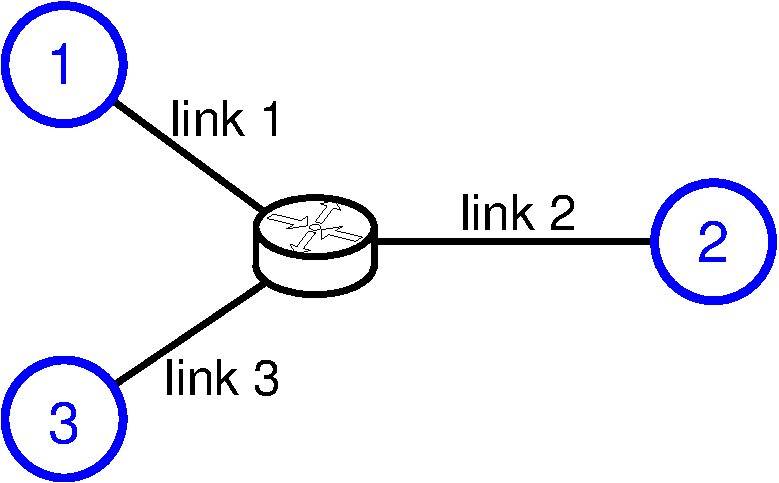
\includegraphics[width=1\columnwidth]{tm_formulation.pdf}
      \caption{Link labels}
      \label{fig:tomo_a}
    \end{subfigure}
    \hfill
    \begin{subfigure}[b]{\twoup}
      \centering
      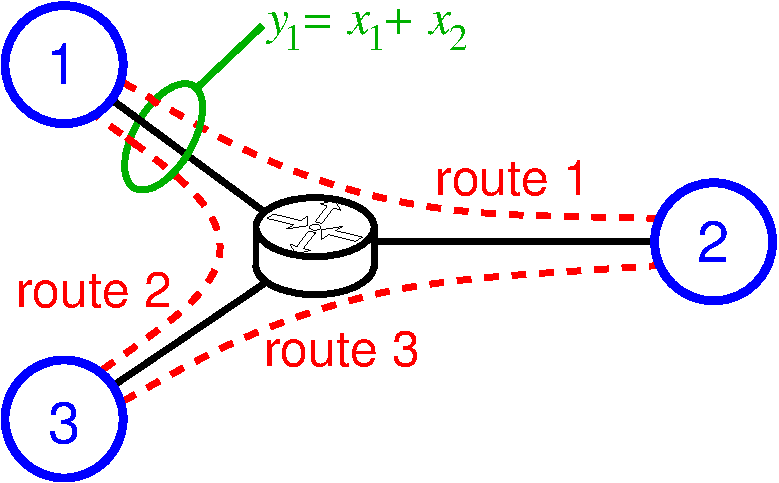
\includegraphics[width=1\columnwidth]{tm_formulation_2.pdf}
      \caption{Traffic labels and routes}
      \label{fig:tomo_b}
    \end{subfigure}  
    \hspace*{3mm}
    
    \caption{A simplified network and traffic (the main
      simplifications are that we only consider a single router, and
      only consider unidirectional traffic, not bidirectional as in
      real networks).\label{fig:tomo}}
  \end{center}
\end{figure}         

All the link counts may be grouped into an $L \times 1$ vector
$\by$. Then, based on link observations in one measurement interval,
the SNMP link counts may be expressed as 
\be 
  \by = \bA \bx,
  \label{eq:observation}
\ee 
where $\bx$ is the $N(N-1) \times 1$ vectorised version of the
traffic matrix $\bX$, with its columns stacked upon one another.  

\autoref{fig:tomo} presents an example of \autoref{eq:observation}. It
shows how the traffic on a single link $y_1$, is built from the sum of
traffic routed across the link $x_1 + x_2$. We can see that by
stacking each of these equations we would get
\be
  \left(\begin{array}{l} y_1 \\ y_2 \\ y_3 \end{array} \right) =
  \left(\begin{array}{lll} 1 & 1 & 0 \\ 1 & 0 & 1 \\ 0 & 1 & 1 \end{array} \right)
  \left(\begin{array}{l} x_1 \\ x_2 \\ x_3 \end{array} \right),
\ee
which, written in matrix notation, is just
\autoref{eq:observation}. Note that in this case the routing matrix
$\bA$ is invertible, so the problem of inferring the traffic matrix from
link measurements is easy, but this is rarely the case. Usually, $L$
is usually much smaller than $N(N-1)$, and so the
problem is highly underconstrained.

There are two main assumptions implicit in this observation model. It
assumes the traffic matrix is stationary, \ie~its statistical
properties remain stable throughout the measurement interval and there
are no errors in the measurement. Stationarity is preserved by
choosing an appropriate measurement interval, say 1 hour (see
\autoref{sec:models}). Moreover, in reality, errors do occur and to
account for it, the model \autoref{eq:observation} is extended to 
\be 
\by = \bA \bx +\bz.
 \label{eq:observation_noise}
\ee 


\noindent The second model is a simple noise additive model often used
to test the robustness of an inference technique. Each element of the
additive noise term $\bz$ is typically chosen to be independent and identically
distributed (i.i.d.) white
Gaussian noise with mean zero and variance $\sigma^2$. Often
$\sigma^2$ is kept small, as large values would result in some
elements of $\by$ violating the non-negativity constraint. It is
for this reason other distributions may be used, for example,
log-normal or gamma distributions. Additionally, due to the problem of
missing link information due to poor SNMP implementation, some of the
elements of $\by$ may be missing. Finally, if the given routing
matrix $\bA$ is incorrect, the observations $\by$ would
significantly depart from the true SNMP link counts. However, most
works assume an accurate $\bA$ because there are reliable methods for
obtaining routing information \cite{Shaikh02OSPF}.

There are usually many less links than the total number of IE pairs,
and so the inverse problem above is highly underconstrained.  Whether
noise is present or not there may be an infinite number of solutions
$\bx$ that fit the observations
\eqref{eq:observation}. \autoref{fig:tomo_hard} shows a picture of
such a network, where we only measure at the bottleneck. Now, even in
this very simple network the equations $y_1 = x_1 + x_2$ are
underconstrained. In order to make progress, some additional
information needs to be assumed, usually in the form of a traffic
matrix model, and we shall consider some of these in the following
section.



\begin{figure}[!thbp] 
  \begin{center}
    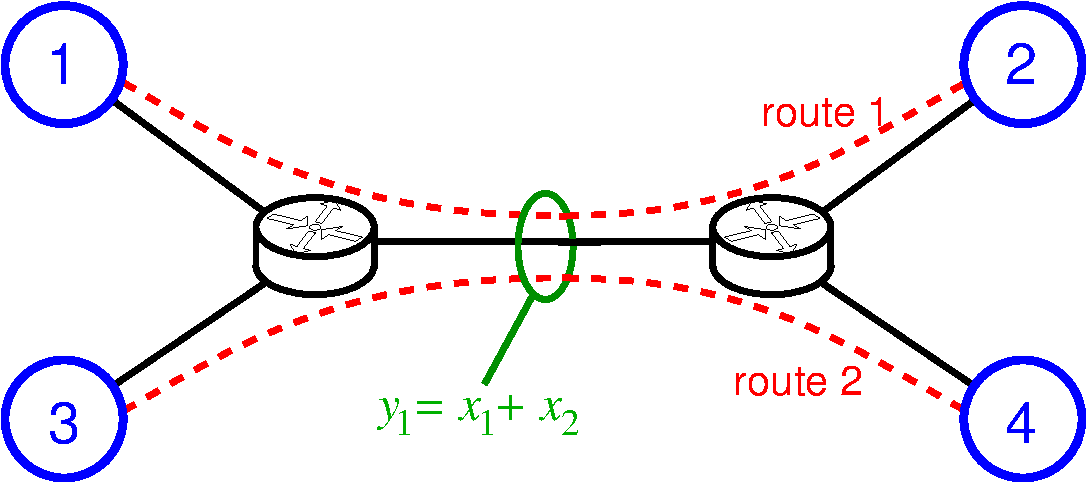
\includegraphics[width=0.6\columnwidth]{underdetermined.pdf}
    \caption{A harder inference problem where we only have one
      measurement, but two traffic elements to estimate. There is
      therefore a fundamental ambiguity in this problem.
      \label{fig:tomo_hard}}
  \end{center}
\end{figure}         

Before moving on to the modelling aspects of traffic matrices, note that
there are other strategies for measurement. For instance, if MPLS is
being used, this creates a set of tables (in many implementations)
that can almost be read directly to obtain the matrix (\eg~see
\cite{blili08:_best_pract_deter_traff_matric}).  Alternatively, the
network operator may have more accurate local traffic matrices,
obtained through specific functionality at the routers. It is, in
principle, easy for a router to keep counts of its decisions
\cite{Varghese03Measure}, essentially amounting to a table of the
volumes of traffic between pairs of interfaces.  Locality here is
defined in the sense of the matrix's restriction to a single router --
we essentially see an IE traffic matrix of the single router's
interface.  These local matrices from all routers in the network can
be used to improve the estimation of the IE traffic matrix; see
\autoref{sec:applications}. On some special cases, such as a star
network, a single local matrix would be equivalent to the traffic
matrix, serving to highlight the information gain from local traffic
matrices. These matrices provide greater than a two-fold increase in
accuracy of the tomography estimation schemes by
\cite{Medina02TMdirections,Zhang03Fast}.



% Model
%\clearpage
\section{Models}
\label{sec:models}

In this section, several canonical as well as recently proposed models
are presented. Modelling is divided into three categories: purely
temporal modelling, spatial modelling and spatio-temporal modelling.
 
\subsection{Temporal Modelling}
\label{ssec:temporal_modelling}

Purely temporal models only focus on the time series properties of the
traffic matrix. A key application of these models is in anomaly
detection, so as to be able to pinpoint the time and location of the
anomalous event. This is especially vital in detecting attacks on the
network or worm outbreaks. However, temporal behaviour is also
important in prediction, say for planning capacity of a future
network.

Before delving into the models, some basic issues regarding the
temporal properties of OD flows need to be understood. It is commonly
agreed that IP data traffic is rising exponentially, and has been for
more than a 
decade~\cite{claffy94:_track_long_term_growt_of_nsfnet,groschwitz94:_time_series_model_of_long,odlyzko03:_internet_growth,cisco_visual_networ_index2011}. There
was much early controversy about such growth estimates, because the
growth rate was vastly overestimated based on a small sample of
data. However, these days, exponential growth is considered the common
case (though with a much lower rate of growth), and is justified both
by data, and as a consequence of increasing computational and
networking speeds, governed by Moore's and Gilder's laws
respectively. As of the present, the introduction of mobile devices
and the rapid growth of traffic from these devices are set to further
increase data traffic in the years to come. Cisco (who admittedly have
a vested interest in a high forecast) estimate that ``Annual global IP
traffic will surpass the zettabyte threshold (1.3 zettabytes) by the
end of 2016''~\cite{cisco_visual_networ_index2011}.

Relatively few countries appear to monitor their national traffic, but
Australia is an exception. The Australian Bureau of Statistics have
collected and published traffic statistics for many
years~\cite{13:_abs_internet}. \autoref{fig:aust_traffic} shows the
growth of traffic in Australia from 2000 to 2012.
 
\begin{figure}[!b]
  \begin{center}
    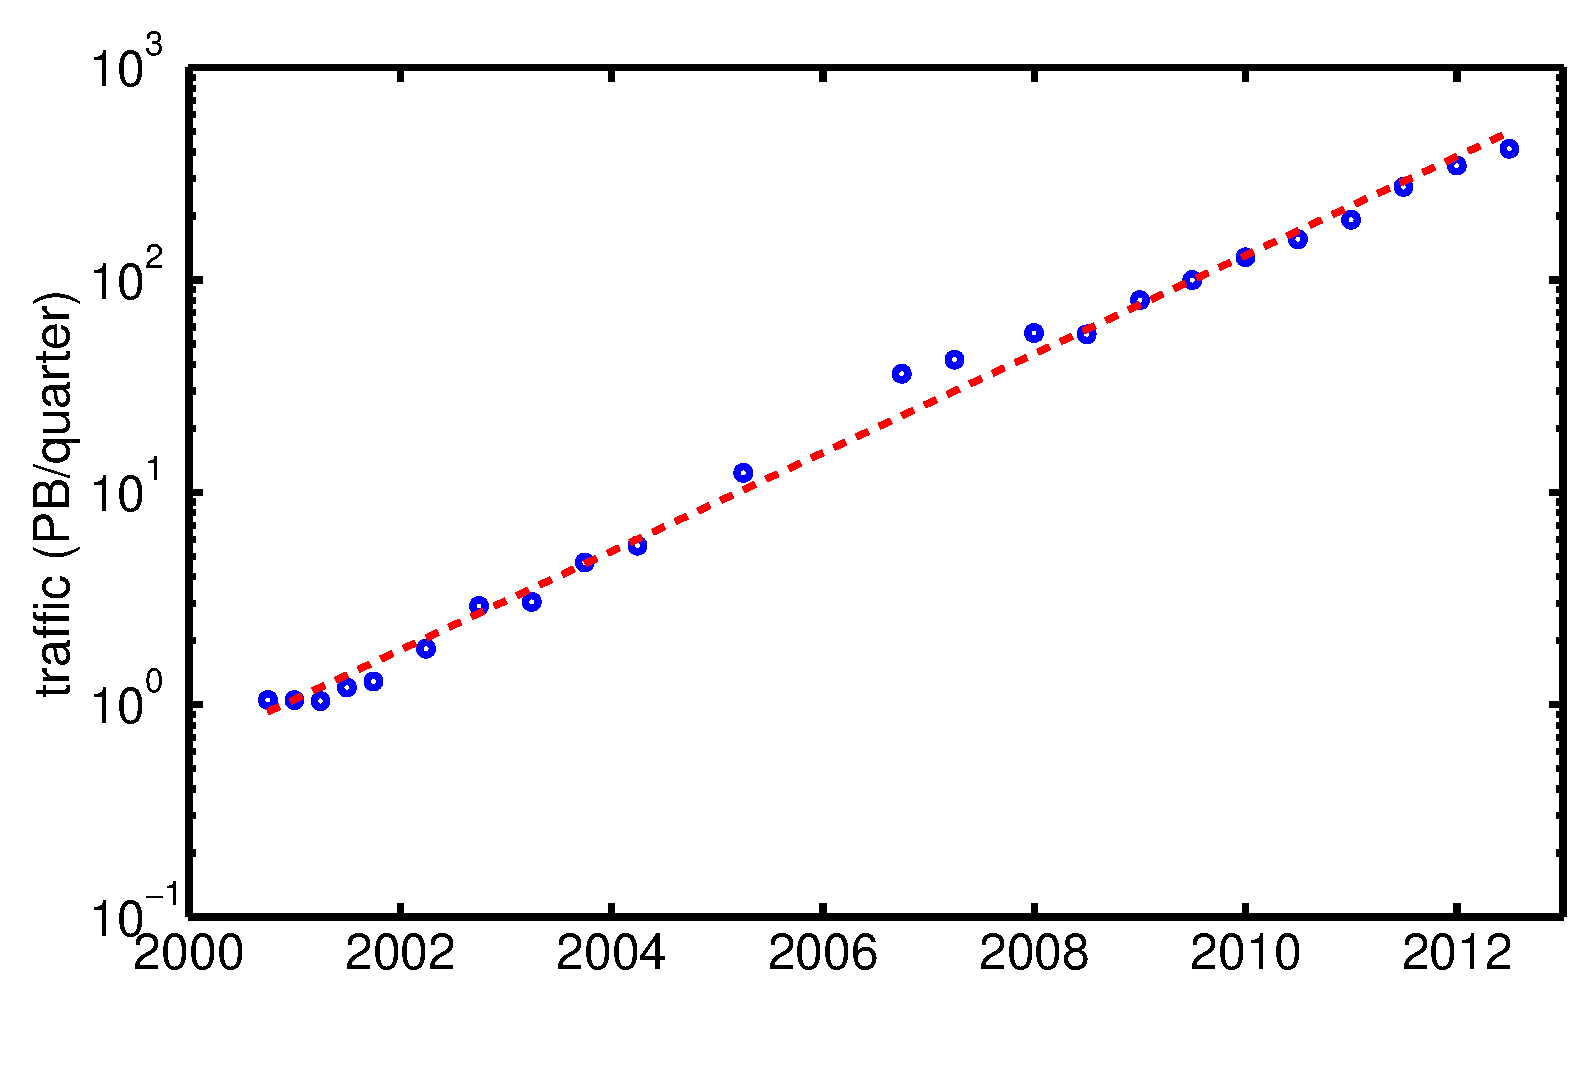
\includegraphics[width=0.7\oneup]{australian_internet_usage_log.eps}
    \caption{Australian Internet traffic volumes based on data from
      the Australian Bureau of Statistics from 2000-2012. The
      dashed line shows a linear fit to the (log) data.  Note
      the log $y$-axis, so the plot shows quite a reasonable fit to
      exponential growth with a doubling period of 465 days. Over the
      same period the growth in broadband subscribers has been almost
      exactly linear (soon this trend must decrease as a large
      proportion of Australia's population are now connected), so most of
      the growth has come from growth in the amount downloaded per customer.
      \label{fig:aust_traffic}}
  \end{center}
\end{figure}

Regardless of your belief about the rate of growth, and/or the best
model (exponential is common, but linear and logistic models may also
be appropriate in many cases), any model of long-term traffic needs to
be able to incorporate such growth.

Second, most network traffic is human generated. Therefore, it stands
to reason that traffic is influenced by human activity in a 24 hour
cycle. In fact, distinct diurnal patterns have been observed, with
peak traffic occurring around mid-day or in the evening and dips
during the night, for example see \autoref{fig:abilene_2004_b}. This
correlates to the daily schedule of an average human being, where
mid-day traffic is generated for work or school purposes, while the
lack of traffic during the night correlates to sleeping periods.  Peak
traffic rate is also noticeably less on the weekends.  The regularity
of this behaviour can be quite strong as shown in the figure where two
successive weeks' data are overlaid so one can see how closely they
match. Most traffic measurements see some measure of cyclic behaviour,
with the degree of regularity determined by the type of traffic (is it
made up of many individuals or a few large flows) and the scale.

% \begin{figure}[thbp] 
%   \begin{center}
%     \hfill
%     \begin{subfigure}[b]{\twoup}
%       \centering
%       \Diurnal
%       \caption{Traffic rate over the span of a single week starting
%         from May 7th, 2001, with the traffic rate of
%         the following week overlaid.}
%       \label{fig:cycle_week}
%     \end{subfigure}
%     \hfill
%     \begin{subfigure}[b]{\twoup}
%       \centering
%       \DiurnalZoom
%       \caption{Traffic rate of a single day,  May 8th
%         2001, on the same ISP, with traffic on  
%         May 15th, 2001 overlaid on top.}
%       \label{fig:cycle_day}
%     \end{subfigure}  
%     \hfill\mbox{ } \\
    
%     \caption{Observations of the cyclicality of the total traffic rate of a large PoP.\label{fig:cycle}}
%   \end{center}
% \end{figure}         


Third, and leading from the last point, the traffic volume itself is
dependent on the measurement period and the aggregation level of
traffic. At very short scales, in milli-seconds or seconds, the
traffic distribution is highly variable, and shows strong
dependencies, making use of such measures statistically non-trivial,
even if such measurements were easy to collect.  A common paradigm is
to consider a measurement interval of minutes to an hour, where
measurement is easy. Also important is the fact that at these times
scales \emph{stationarity}\footnote{Stationarity refers to the concept
  that the statistics of the traffic (for instance, the mean and
  variance, but in general including all statistics) are constant with
  respect to the time at which they are measured. Wide-sense
  stationarity is when only the mean and variance of the traffic
  satisfies the stationarity property.  In Internet traffic data it is
  only ever approximately true.  Moreover, it is hard to test for
  stationarity when traffic has long-term correlations, and so we can
  only ever talk about the degree of stationarity.} of the traffic
volume distribution is often a reasonable assumption, though we can
see the limits of this in \autoref{fig:abilene_2004_b} (stationarity clearly
doesn't hold for more than a couple of hours), however it was shown
that {\em cyclo-stationarity} holds to a large extent
\cite{Soule04TMLargest}.

Fourth, there are natural variations in traffic over time, and these
are often modelled as a random (or stochastic) process. This random
process could have all sorts of features, but there are some basics
that should be observed by all reasonable models. For instance,
network operators aggregate traffic from multiple sources, which is
known as \emph{multiplexing}. Multiplexing is used to boost the
efficiency of the links in a network by ``smoothing'' out variations
in traffic. The apparent smoothness is a result of decreases in the
relative variance, as predicted by the central limit
theorem~\cite{Cao01Nonstationarity}.  The more OD flows multiplexed on a
link, the higher the efficiency and smoothing effect, provided the
aggregated bandwidth does not exceed link capacity. Thus, any model
for the large traffic rates in a network must be consistent under
multiplexing, for example, when the number of flows being multiplexed
is increased the relative variance should decrease in a predictable
manner. Furthermore, the statistical properties of the aggregated
traffic must also be consistent with the statistical assumptions of
the traffic from a single user.

Finally, although rare, sometimes there may be sudden ``spikes'' in
traffic.  Such a component may arise from unusual traffic behaviour,
such as DDoS attacks, worm propagation or Border Gateway Protocol (BGP) 
routing instability from misconfiguration. Flash crowds are also an example of this behaviour,
which happens when there is a significant jump in the number of
clients to a particular web server or CDN. 
Extreme unforeseen events, such as the September 11 attacks on
the World Trade Centre in 2001 may instead cause a significant drop of
traffic rates. In any case, a massive shift in traffic rates would be
of interest to a network operator.

One temporal model of OD flows traversing backbone routers was
proposed by Roughan \etal~\cite{Roughan02BRvariable} by generalising
the Norros model \cite{Norros94Storage}, originally used for modelling
LAN traffic. Each OD flow is assumed to be generated from an
independent source. The model is characterised by the following
components (at time $t$):
\begin{enumerate}
\item $L(t)$, the long term traffic trend,
\item $S(t)$, the seasonal (cyclical) component, 
\item $W(t)$, random fluctuations, and
\item $I(t)$, the anomaly component.
\end{enumerate}
These components correspond to the observations of traffic described earlier.

The long term trend, $L(t)$, depends on the observed underlying
traffic growth in the data. This factor captures the overall growth of traffic over
a long time period. An exponential growth model for instance,
could be found by fitting $L(t) = A \exp(ct)$ to the data, with the
parameters $A$ and $c$ easily estimated via log-linear regression as
in \autoref{fig:aust_traffic}. 

The component $S(t)$ may be any periodic function, such that
$S(t+kT_s) = S(t)$ for all integers $k$, where the period $T_s$ would
typically be 24 hours, or one week. 

The component $W(t)$ is assumed to be a stochastic process with
zero mean and unit variance, to model the small fluctuating component of 
observed traffic. Finally, $I(t)$ captures the large variability of traffic from
anomalies, say, a massive upsurge or downsurge in traffic. These events were 
captured in an individual component to separate their influence from 
traffic under the network's normal operating conditions.

Let $x(t)$ denote the volume of an OD flow at time $t$. The model
takes the following form, 
\be 
  x(t) = m(t) + \sqrt{a m(t)} W(t) + I(t),
  \label{eq:temporal_model}
\ee 

\noindent where $m(t) = S(t)\,L(t)$ is the mean of the OD flow,
assumed to be a product of the seasonal and long term trends, and $a$
is the \emph{peakedness} of the traffic. The average is modelled in
such a way because as large OD flows have a larger range of variation
in the size of their cycles. The parameter $a$ controls the smoothness
of the OD flow's volume in a way that is consistent given multiplexing
of aggregated flows.

\autoref{fig:decomposition} shows the decomposition in action on the
set of Abilene data shown in \autoref{fig:abilene_2004_b}, extending
the analysis beyond into the section of missing data. The estimated
long-term trend $\hat{L}(t)$ is not shown as it is almost constant
over this period, but we show the estimated mean $\hat{m}(t)=
\hat{S}(t)\, \hat{L}(t)$ (derived using a 5 term seasonal moving
average, further smoothed with a 13 term moving average), shown in
green. Normal bounds on this, obtained by modelling the random
fluctuations $W(t)$ as a Gaussian process are shown as dashed lines,
and where the traffic falls outside these bounds, we have indicated an
anomaly. 

We have deliberately looked at this period, which is followed by
period of missing data to illustrate one of the advantages of this
approach, which is the ability to fill in missing gaps in the data,
though more sophisticated approaches to solve that problem also
exist, \eg~see \cite{Zhang09TMCS}.
 
\begin{figure}[htp]
  \begin{center}
    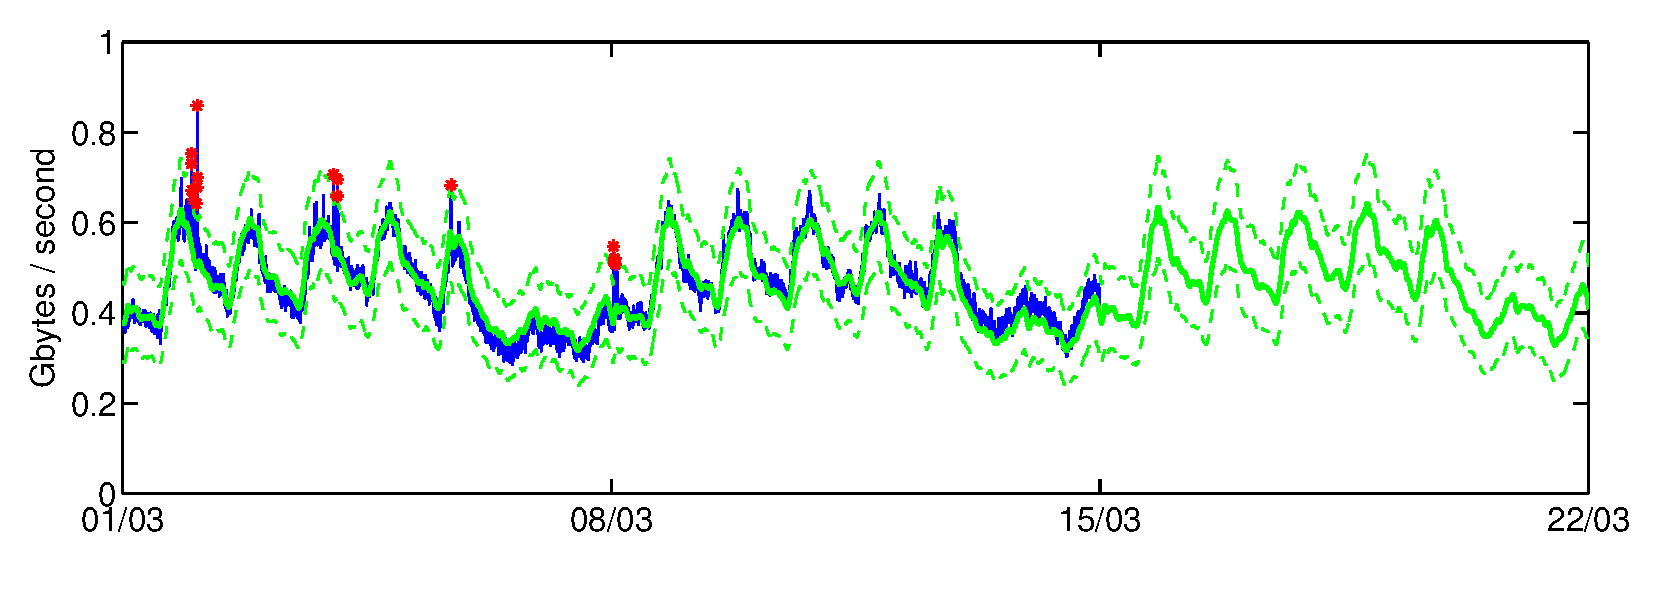
\includegraphics[width=\oneup]{Abilene_2004_decomp_1.eps}
    \caption{Results of decomposing traffic into components. The blue
      curve shows the original Abilene traffic from
      \autoref{fig:abilene_2004_b} (note that the data is missing for
      the third week). The solid green line shows $\hat{m}(t)=
      \hat{S}(t)\, \hat{L}(t)$, the estimated  mean, and the dashed
      green lines show the bounds of normal variation around this
      mean. The red asterisks indicate the anomalies $I(t)$.
      \label{fig:decomposition}}
  \end{center}
\end{figure}

Another feature of this model is the preservation of the properties of the
model through a linear combination, advantageous when looking at the
aggregated behaviour of the OD flows. Consider $K$ aggregated OD
flows, then 
\[
  x_{\text{agg}}(t) = \sum_{i=1}^K m_i(t) + \sum_{i=1}^K \sqrt{a_i m_i(t)} W_i(t) + \sum_{i=1}^K I_i(t). 
\]

\noindent The mean of $x_{\text{agg}}(t)$ is simply $m_{\text{agg}}(t)
= \sum_{i=1}^K m_i(t)$, and the peakedness is the weighted average of
the component peakedness, $a_{\text{agg}} =
\tfrac{1}{m_{\text{agg}}(t)} \sum_{i=1}^K a_i m_i(t)$. The linearity
properties allow $x_{\text{agg}}(t)$ to be expressed in the same form
as \autoref{eq:temporal_model} with the new parameters
$m_{\text{agg}}(t)$ and $a_{\text{agg}}$. The linearity property
enables the consistent computation of the variances of the aggregated
traffic, which is useful for network planning and analysis. Besides
this, \cite{Roughan02BRvariable} demonstrated the ease of estimating
the parameters of model \autoref{eq:temporal_model}, via simple
estimators and filtering.

The cyclical nature of the aggregated OD flows is also amenable to
Fourier analysis. The Fourier transform decomposes a periodic signal
into a weighted sum of sinusoids with distinct frequencies and
phases. It would be reasonable to assume the observed cycles can be
represented by a small number of Fourier coefficients (this does not
require that the signal be exactly sinusoidal as any periodic signal
can be approximated by a limited number of sinusoids). Indeed, it has
been demonstrated this is the case with the traffic volumes
\cite{Soule04TMLargest,eriksson10:_basis}, where as little as just
5 Fourier coefficients were needed to achieve low error in fitting
large OD flows of a Tier 1 network, demonstrating the relatively few
significant frequencies present in a diurnal cycle of the OD
flows. 

\autoref{fig:fourier} shows a similar analysis of Abilene data from
\autoref{fig:abilene_2004_b}. It shows a simple example of the
excellent degree of approximation to traffic we can obtain using only
a very small number of Fourier coefficients corresponding to daily
periods. 
\begin{figure}[thbp] 
  \begin{center}
    \mbox{ }\hfill
    \begin{subfigure}[b]{\twoup}
      \centering
      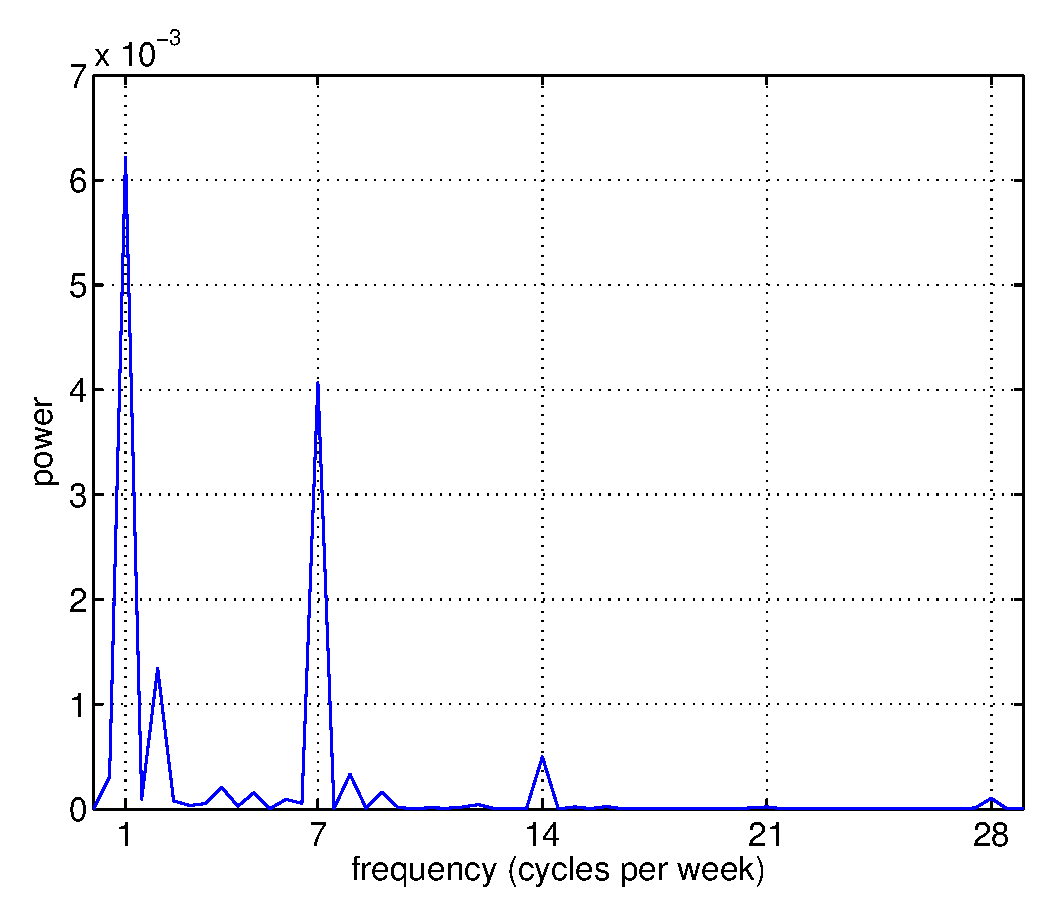
\includegraphics[width=\textwidth]{Abilene_2004_fourier_sprectra.eps}
      \vspace{-5mm}
      \caption{Fourier spectra (technically a periodogram) of the
        Abilene data.}
      \label{fig:fourier_a}
    \end{subfigure}
    \hfill
    \begin{subfigure}[b]{0.47\textwidth}
      \centering
      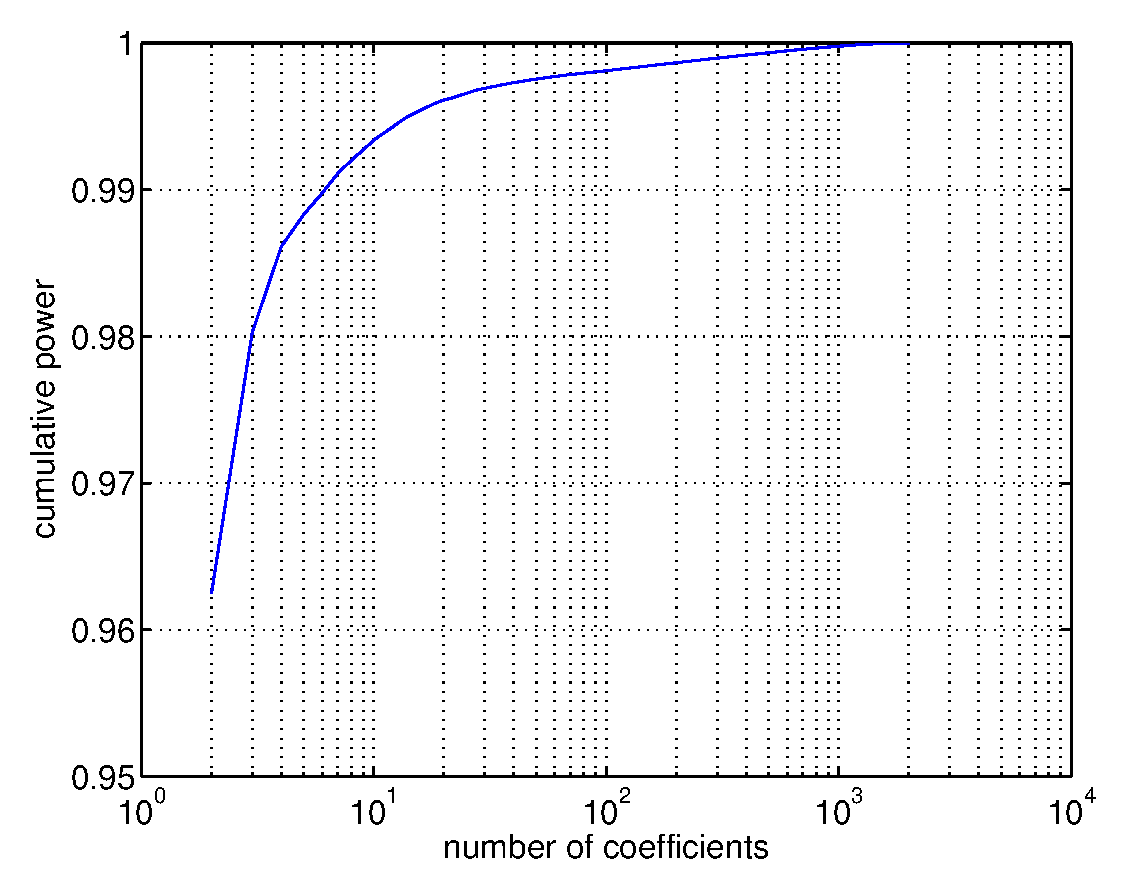
\includegraphics[width=\textwidth]{Abilene_2004_fourier_cum_power.eps}
      \vspace{-5mm}
      \caption{Cumulative power captured by Fourier components
        (sorted in descending order).}
      \label{fig:fourier_b}
    \end{subfigure}  
    \hfill \mbox{ }

      \vspace{5mm}
    \begin{subfigure}[b]{\oneup}
      \centering
      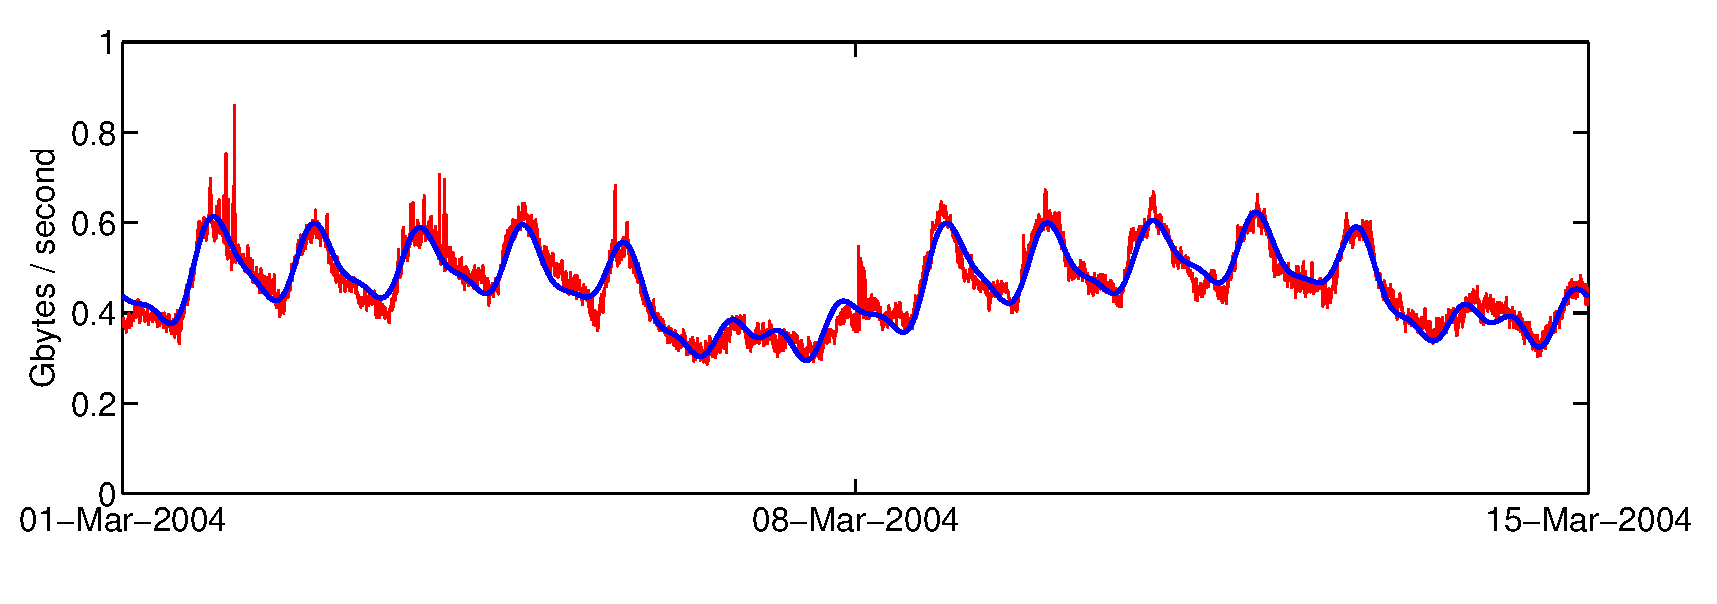
\includegraphics[width=\textwidth]{Abilene_2004_fourier_model_10.eps}
       \vspace{-9mm}
     \caption{Fourier approximation to the data using 10 (complex) coefficients.}
      \label{fig:fourier_c} 
    \end{subfigure}  

      \vspace{5mm}
    \begin{subfigure}[b]{\oneup}
      \centering
      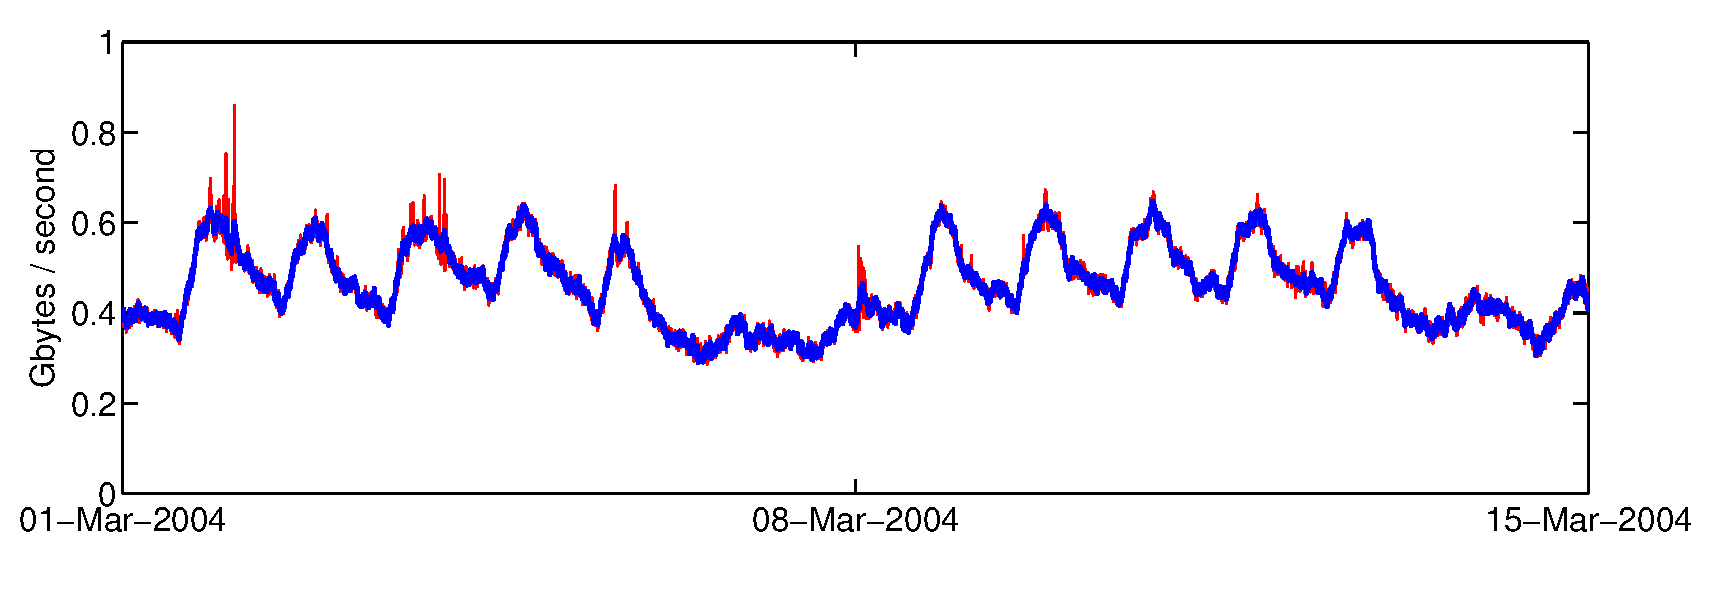
\includegraphics[width=\textwidth]{Abilene_2004_fourier_model_100.eps}
      \vspace{-9mm}
      \caption{Fourier approximation to the data using 100 (complex) coefficients.}
      \label{fig:fourier_d}
    \end{subfigure}  
   
    \caption{Fourier analysis of Abilene data shown in \autoref{fig:abilene_2004_b}. Blue curves represent the
    Fourier approximation of the traffic, indicated by the red curves.\label{fig:fourier}}
  \end{center}
\end{figure}         
\autoref{fig:fourier_a} shows the periodogram of the data
(the absolute magnitude of the Discrete Fourier Transform (DFT)). We
can see that only a few peaks (with frequencies of 1, 2, 7, and 14
cycles per week, corresponding to daily and weekly cycles and their
harmonics) are large enough to matter for gross features.
\autoref{fig:fourier_b} shows the cumulative power contained in the
largest of the Fourier coefficients, clearly showing that a small
number of these represent the power of the signal
well. \autoref{fig:fourier_c} shows an approximation of the original
signal using only 10 coefficients. We can see that the cyclic
components of the data are represented well, though the actual signal
varies around that noisily. Including additional components provides a
better approximation (in the sense of fitting the data more
accurately), but we can see that we are simply recreating the
noise. There is a clear tradeoff here between noise and signal, with
no absolute standard for the correct choice, but the underlying
promise of Fourier analysis is obvious.

The choice of time interval to use in Fourier analysis/approximation
is interesting. A longer interval provides more data, and hence better
estimates if the data is truly {\em cyclostationary}\footnote{A
  cyclostationary process can be thought of as one whose component
  processes formed from times embedded at multiples of the fundamental
  period from stationary sequences.}. However, as we discussed earlier, 
  there are noticeable
% http://en.wikipedia.org/wiki/Cyclostationary_process
trends in the overall volume, and so it is reasonable to assume that
there will sometimes be significant shifts in the pattern (with
respect to time of day or time of week). In these cases, extending the
length of the dataset can confuse the statistical variability with
non-stationary effects, resulting in biased estimates. The best
tradeoff appears to depend on the dataset, but periods of perhaps a
month seem to work reasonably well for estimating weekly cycles. 

However, there are alternative tools for such analysis, designed to
provide some flexibility in the tradeoff between time and
frequency. The simplest is perhaps the Short-Time Fourier Transform,
in which the signal is {\em windowed}, and the standard DFT is applied
to the windows of data to produce a {\em spectrogram}. The technique
has been applied in \autoref{fig:spectrogam} to a longer (6
weeks) sequence of the Abilene data. This segment of the data is more
challenging, as it contains many anomalies, \eg~the frequent spikes
in the traffic, or the drop in traffic on the Independence Day holiday,
observed on July 5th in 2004\footnote{Independence Day is actually 
celebrated on July 4th, but in 2004, the day falls on a Sunday. Thus, the following
day was declared a public holiday as well.}. \autoref{fig:spectrogam_a} shows the
set of data under consideration, along with its approximation using 10
coefficients. \autoref{fig:spectrogam_b} shows a spectrogram with
windows of length 1 week, and here we can still clearly see the weekly
and daily cycles appearing in most of the
windows. \autoref{fig:spectrogam_c} shows a spectrogram using 1 day
windows, with overlapping windows to smooth the results. The resulting
picture is poor at showing the cyclical behaviour of the traffic, but
clearly highlights the large anomalous spikes in the traffic in second
week of the data. 

\begin{figure}[thbp] 
  \begin{center}
    \begin{subfigure}[b]{\oneup}
      \centering
      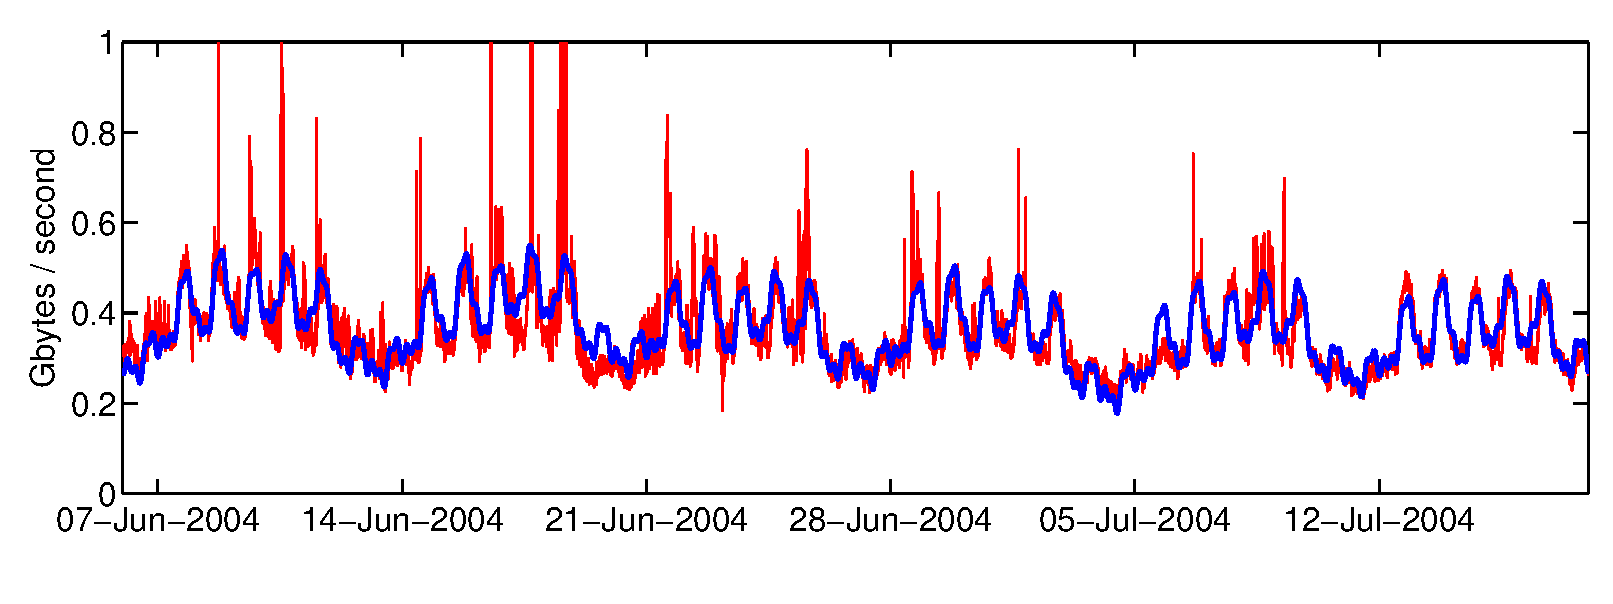
\includegraphics[width=\textwidth]{Abilene_2004_spectrogram_input.eps}
       \vspace{-9mm}
     \caption{Six weeks of Abilene data.}
      \label{fig:spectrogam_a} 
    \end{subfigure}  

      \vspace{5mm}
    \begin{subfigure}[b]{\oneup}
      \centering
      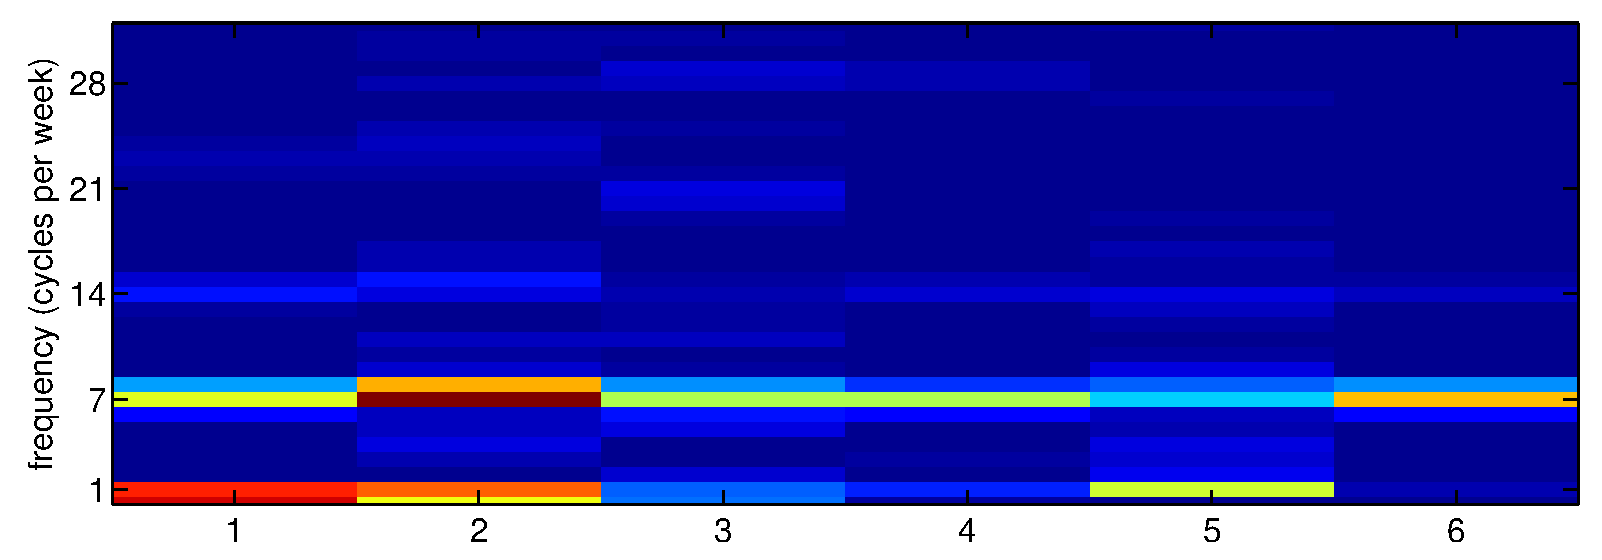
\includegraphics[width=\textwidth]{Abilene_2004_fourier_spectrogram_week.eps}
       \vspace{-5mm}
       \caption{Spectrogram with weekly windows. Brighter colours
         indicate more power. Again we see strong power at 1 and 7
         cycles per week, though the strength of these varies per
         week. For instance, in week 5 (when the Independence Day
         holiday was held) there was a week day, whose traffic more
         closely resembled weekend traffic, breaking the weekly cycle,
         and pushing more power into the daily cycle.}
      \label{fig:spectrogam_b} 
    \end{subfigure}  

      \vspace{5mm}
    \begin{subfigure}[b]{\oneup}
      \centering
      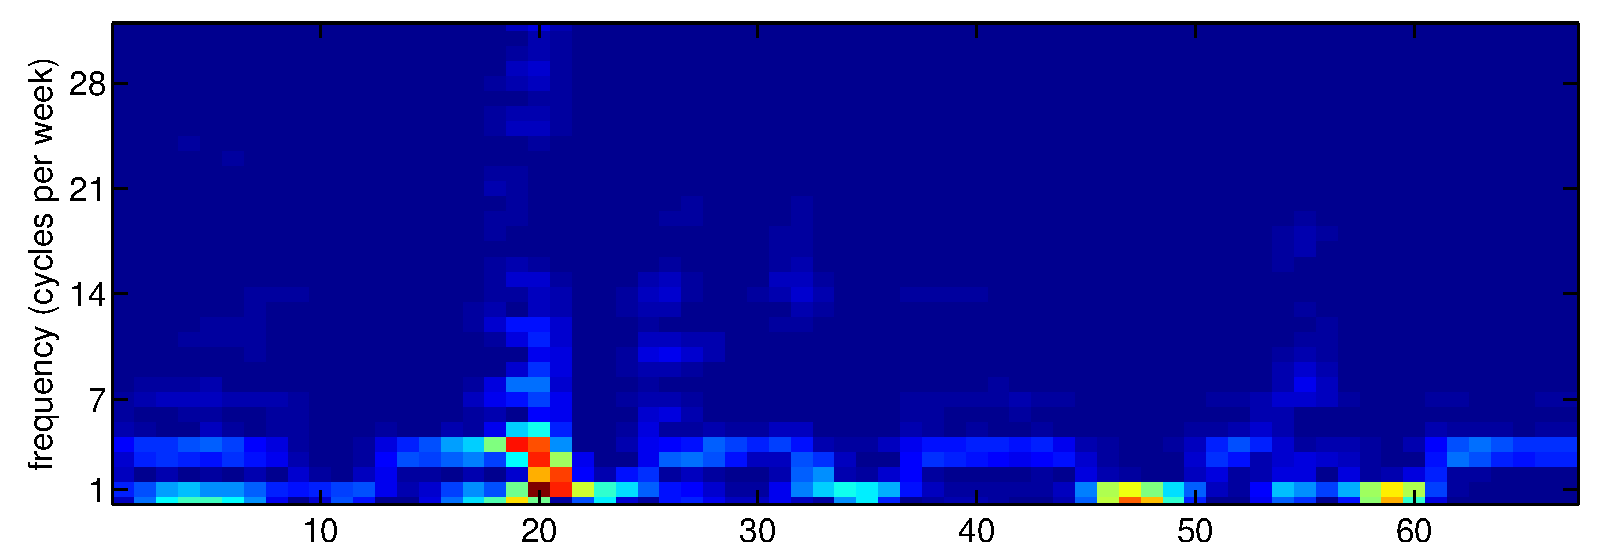
\includegraphics[width=\textwidth]{Abilene_2004_fourier_spectrogram_day.eps}
      \vspace{-5mm}
      \caption{Spectrogram with daily windows. Note that the
        time-resolution in this case is actually poorer than the image
      would suggest, accounting for the poor resolution of the daily
      and weekly cycles in this figure. However, the large anomalous
      spikes of traffic in the second week stand out clearly in this
      view, as they spread power across a range of frequencies.}
      \label{fig:spectrogam_c}
    \end{subfigure}  
   
    \caption{Short-Time Fourier analysis of Abilene data.\label{fig:spectrogam}}
  \end{center}
\end{figure}         

An even more powerful set of techniques that have been applied to the
temporal analysis of traffic are the Wavelet
transforms~\cite{Veitch97Wavelet,Barford02Anomaly,Papagiannaki05Long},
which provide a more flexible set of time/frequency
tradeoffs. Wavelets have also been applied to spatial analysis of
traffic matrices 
\cite{CrovellaKolaczyk03,CoatesCompressedNetworkMonitoring,wang10:_wavel_based_traff_matrix_model,rincon08:_dw,roughan_mra_09},
which we will consider in a moment.  However, wavelets are a
relatively complicated set of techniques, and it is outside the scope
of this chapter to provide an introduction to that material. See for
instance \cite{mallet:_book} for more information. 

Principal components analysis (PCA) has also been employed to quantify
the temporal correlations of the traffic matrix. If $\cX$ is a matrix
where the rows represent a measurement (for instance an OD flow) and
columns represented traffic volumes at time $t$, then temporal PCA
decomposes the matrix $\cX^\T \cX$ into its corresponding components
of eigenvalues and eigenvectors. Often, each column is \emph{centred}, simply by
subtracting the mean vector $\bar\bx$, the average of all columns, from each 
column in $\cX$. In what follows, $\cX$ is assumed to be centred.

The matrix $\cX^\T \cX$ is \emph{positive
semidefinite}. Visualising this geometrically, if the columns of the matrix is reinterpreted
as a set of points, then they trace out an ellipsoid. Alternatively, $\cX^\T \cX$
may be viewed as the \emph{empirical covariance matrix} of the columns of
$\cX$, in effect computing temporal correlations in traffic. 

PCA is used to find the directions of greatest variance of $\cX^\T \cX$
by decomposing $\cX^\T\cX = \bW \bD \bW^\T$, where $\bW$ is an orthonormal matrix 
containing the eigenvectors of $\cX^\T\cX$ and $\bD$ the diagonal 
matrix containing the eigenvalues of $\cX^\T\cX$. The eigenvectors
are known collectively as the \emph{principal axes}. The eigenvectors are ordered in a 
non-decreasing order with respect to their associated eigenvalues, starting from the
eigenvector associated with the largest eigenvalue to the smallest. An equivalent view
is that PCA essentially performs a Singular Value Decomposition (SVD) of the matrix
$\cX$, by computing only its right singular basis $\bW$.

Thus, every row of $\cX$ can be expressed as $\bx_k =  \baa^\T_k \bW^\T$, 
\ie~a linear combination of a coefficient vector
$\baa_k$, called the \emph{principal components}. Here, $\bW$ is equivalent to a linear
transform, post-multiplied to the data. Intuitively, if the size of the set of
principal axes with large principal components are small, then this is evidence
there are high temporal correlations between the traffic flows. In practice, it is
common to focus on the few largest principal axes for the purpose of data reduction.
Basically, this means choosing the first few significant columns of $\bW$ to approximate each
$\bx_k$ with $\tilde\bx_k$ such that $\|\bx_k - \tilde \bx_k\|_2 < \epsilon$, for some 
small error $\epsilon > 0$.

As an aside, PCA may be performed on $\cX\cX^\T$, in effect computing the spatial
correlations of $\cX$ instead. Here, we have $\cX\cX^\T = \bV \tilde\bD \bV^\T$, with
each column $\bar\bx_k = \bV \tilde \baa_k$, equivalent to $\bV$ pre-multiplied
with the data. Spatial PCA was used in the context of anomaly detection
\cite{Lakhina04Anomaly,Lakhina04Diagnosing,Lakhina05Mining} but there are problems
with this approach. These discussions are deferred to \autoref{sec:applications}.

\begin{figure}[thbp] 
  \begin{center}
     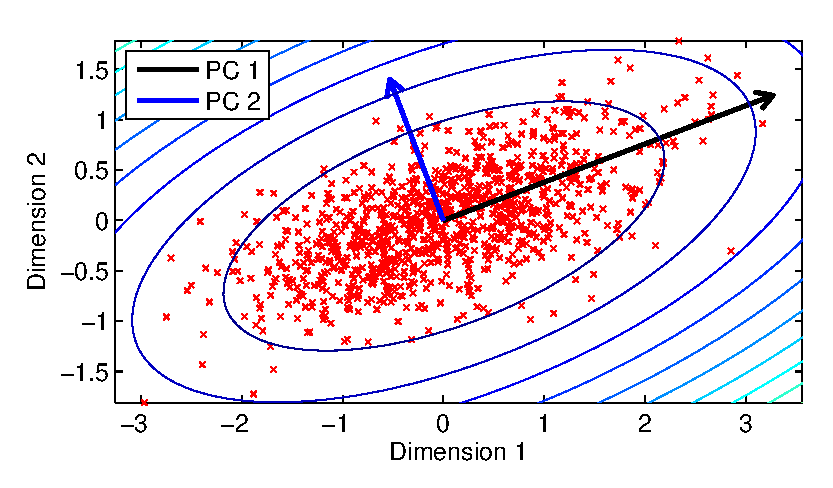
\includegraphics[width=0.7\textwidth]{PCA_example.eps}
    \caption{Principal components analysis of the empirical covariance matrix of a two dimensional 
    data matrix of 1000 centred points $\cX$. Here, ``PC 1''  and ``PC 2'' are the principal 
    components. Note the elliptical shape of the contours of the
    density with semi-major and semi-minor axis given by the first and
    second principal components, respectively.  \label{fig:pca}}
  \end{center}
 \end{figure}
 
\autoref{fig:pca} demonstrates an example of PCA performed on the covariance matrix of 
1000 two dimensional data points with zero mean, \ie~$\cX$ has 2 rows and 1000 columns. 
The matrix $\cX^\T \cX$ formed by the data points vaguely resembles an ellipse. Here, there
are two principal components, denoted by  ``PC 1''  and ``PC 2'', with the higher variance
captured by PC 1. This is clear from the way the points on the figure
are distributed. The key point to take away is that both components capture the direction
of highest variance and are orthogonal to each other.  Moreover, the principal components matrix 
$\bW$ has PC 1 and PC 2 as its first and second columns respectively. Each data point 
can be expressed as linear combination of these two components. The concept is easily
extended beyond two dimensions to the larger dimensions typically encountered with
traffic matrices.

PCA was performed by Lakhina \etal on empirical data from two backbone networks show
that OD flows are a combination of no more than 35 ``eigenflows'' (the principal axes), and
in fact, fewer than this in general \cite{Lakhina04TrafficStruct}, out of over 100 OD flows. 
These eigenflows belonged to one of three categories, depending on their properties:
\begin{enumerate}
\item \textbf{deterministic or $d$-eigenflow}: generally the
  significant diurnal component of the largest OD flows. Although
  present in smaller OD flows, these eigenflows are less
  significant. These eigenflows have a cyclo-stationary property and
  suggests that these eigenflows may be approximated by a small number
  of Fourier coefficients. These eigenflows account for the majority
  of the total traffic of the OD flow.
\item \textbf{spike or $s$-eigenflow}: medium sized eigenflows with a
  spikiness behaviour in time, with values ranging up to 5 standard
  deviations from the mean of the OD flow. This suggests these
  contributions come from bursty processes and may be modelled by a
  wideband Fourier process.
\item \textbf{noise or $n$-eigenflow}: small eigenflows behaving like
  stationary additive white Gaussian noise. These eigenflows have
  small energy and their contribution to overall traffic is
  negligible. The majority of eigenflows from Lakhina {\em et al.}'s datasets
  belong to this category.
\end{enumerate}
There are several eigenflows belonging to two or more categories, but
these eigenflows are rare \cite{Lakhina04TrafficStruct}.  For the most
part, these categories are very distinct for almost all
eigenflows. The low number of eigenflows compared to the dimension of
the traffic matrices under study suggests low intrinsic dimensionality
of traffic matrices, although the upper bound of 35 eigenflows indicates that the OD traffic
is only ``approximately'' low rank. The results show a power law-type distribution
of the principal components \cite{Lakhina04TrafficStruct}. The decay of the
distribution varies depending on the ISP, with some distributions
exhibiting a very fast decay and some much slower decay.

In many senses PCA confirms the previous analysis
and modelling, but it is interesting because its approach simply looks
for correlations across different sets of measurements, and uses a
different set of assumptions from, for instance, Fourier analysis
which can be performed on a single time series.

Finally, it is important to note that the full data needs to be
available (no missing entries in $\cX$) in order to perform
PCA. Furthermore, the basic flavour of PCA as described above is not a
robust method, since it is an entirely data driven method and is
therefore sensitive to outliers~\cite{Ringberg07PCA}. Robust variants
have been proposed but they necessarily complicate the basic version
of PCA presented here, since these modifications entail constructing
methods to identify and exclude outliers. Despite these disadvantages,
in its purest form, PCA is a useful tool to learn the temporal
structure of traffic flows.

\subsection{Spatial Modelling}

Spatial models only focus on the properties of traffic between source
and destination pairs, typically within a single measurement interval,
without regard to how the traffic changes in time. The models
presented here are the gravity model and its generalisations, the
discrete choices model, the independent connections model and low rank
spatial model. However, we shall start with the simplest test models. For ease of
exposition in this section, the set of sources and destinations are
assumed to be sets of PoP ingress and egress nodes, denoted by $\cI$
and $\cE$ respectively. The set $\Omega$ represents the set of all
nodes in the network, \ie~$\Omega = \cI \cup \cE$.

\subsubsection{Simple {\em test} models}

We must remember that the purpose of models is not always to
``realistically'' represent a network's traffic. Their purpose is to
provide inputs to other tasks. One common task is to assess the
sensitivity of a network to different types of traffic, and to that
end, engineers can consider the effect of various artificial {\em test}
models. 

Three such are the uniform traffic model, peak load model, and
focussed overload model. They are extremely simple:
\begin{description}
\item[uniform] this simple model assigns the same value to all
  traffic matrix elements. It is used to provide a base load in some
  experiments, or to see the behaviour of a network under one extreme
  (the most uniform extreme) of traffic \cite[Chapter 4.5.1]{Cahn98WANDesign}.

\item[peak load] this model is equally simple, and equally extreme. It
  has zero for all loads except one OD flow. It simulates the opposite
  extreme where the aim is to see the effect of one dominant flow.

\item[focussed overload] this type of traffic matrix simulates the effect of a
  {\em focussed overload}, or {\em flash crowd}\footnote{See also the
    slashdot effect.}, where many users become interested in one
  location or resource and the traffic to this single location from
  all other sources is the dominant effect in the network. As a
  result, the focussed overload can be represented by a matrix with all
  elements zero, except for one row. We can likewise represent a
  focussed traffic load arising from a single point (say as response
  traffic to a focussed set of queries) by a matrix with a single
  non-zero column.
\end{description}
The advantage of each of the models lies in its simplicity. The
simplicity means that the effect of the traffic is easy to interpret,
and thus gain insights from these models where a more complex
model would perhaps confound us with multiple potential causes for
some results. For instance, in each of the above models we can
gradually increase the traffic to see when capacity bounds are
reached, and where those bounds would be reached in order to identify
potential bottlenecks in a network.

Other test models based on classical distributions such as the Poisson
and Gaussian distributions were proposed by Vardi \cite{Vardi96Tomo},
and Tebaldi and West \cite{Tebaldi98Tomo} and Cao \etal 
\cite{Cao00Tomo}, respectively. Their well-known properties make it easy
to analyse results and provide insights, at the cost of a departure from 
real traffic properties.

\subsubsection{Gravity model}

The gravity model is perhaps the next simplest type of model, but it
has a great deal to offer. Here, traffic from the source to the destination
are modelled as a random process. In its simplest form it assumes, any
packet originating a source to a destination nodes are \emph{independent}
of other packets. 
Depending on context, this could be the origin and destination, or ingress
and egress nodes respectively.  Consequently, the traffic between 
two nodes is \emph{proportional} to
the total traffic from the source node to the destination node. The
gravity model is amongst one of the most well-studied
models and is considered a canonical first generation model.

The name of the model derives from Newton's model of gravitation,
where the gravitational force is proportional to the product of the
mass of two objects divided by the distance between them squared. The
general formulation of the gravity model is defined by two forces: the
\emph{repulsive} force (factor) $R_i$, associated with ``leaving''
from $i$ and the \emph{attractive} force (factor) $A_j$, associated
with ``going'' into $j$. Its general form is described by the
following equation: \be X_{i,j} = \frac{R_i \,A_j}{f_{i,j}},
\label{eq:grav_model}
\ee where $f_{i,j}$ represents the \emph{friction factor}, which
describes the weakening of the forces (akin to distance in Newton's
model), depending on the physical structure of the modelled
phenomenon. The model has been used extensively in various fields, for
instance the modelling of street traffic~\cite{potts72}. 
 
In the context of Internet traffic matrix modelling, the friction
factors have typically been taken to be constant. That is, distance is
assumed to have little effect on network traffic. That certainly
seemed to be true even at a fairly large scale in the past, but it is
unknown to what extent the deployment of CDNs (Content Distribution
Networks) over the last few years has changed distance dependence, 
since CDNs locate traffic closer to the end user to avoid paying for
transit costs across the network, or
how inter-country matrices are affected by distance (for instance
through language barriers). Where distance is ignored, equation
\autoref{eq:grav_model} becomes 
\be X_{i,j} =
\frac{X_i^{\text{in}}\, X_j^{\text{out}}}{X^{\text{total}}},
\label{eq:network_grav}
\ee
where $X_i^{\text{in}}$ is the total traffic entering the
network through $i$, $X_j^{\text{out}}$ is the total traffic exiting
the network through $j$ and $X^{\text{total}}$ is the total traffic
across the network \cite{Zhang03Fast}. The model can be expressed
succinctly as the single rank matrix 
\be 
\bX =
\frac{\bx^{\text{in}}\, \left.\bx^{\text{out}}\right.^\T}{X^{\text{total}}}.
\label{eq:network_grav_mtx}
\ee
The popularity of the model stems from the ease of
estimating the $X_i^{\text{in}}$ and $X_j^{\text{out}}$ for each node
pair $(i,j)$, and especially at the PoP or backbone level, since the
level of traffic aggregation mitigates errors in the estimation of
these quantities from sampled traffic.

The gravity model only captures the spatial structure of the
traffic. The key assumption of the gravity model is the independence
between each source $i$ and destination $j$. Coupled with the
assumption that none of the nodes act as a source or sink of traffic
(\ie~that traffic is conserved in the network) $X^{\text{total}} =
\sum_{k \in \cI} X_k^{\text{in}} = \sum_{\ell \in \cE}
X_\ell^{\text{out}}$. Under normal operating conditions in most
backbone routers, where congestion is kept to a minimum, the
conservation assumption appears reasonable. With this assumption,
\be
X_{i,j} = X^{\text{total}}\, p_i^{\text{in}}\, p_j^{\text{out}},
\label{eq:network_grav_normalised}
\ee
where
\ben
p_i^{\text{in}} 
    = \frac{X_i^{\text{in}}}{\sum_{k \in \cI} X_k^{\text{in}} },
\quad \mbox{ and } \quad 
p_j^{\text{out}} 
    = \frac{X_j^{\text{out}}}{\sum_{\ell \in \cE} X_\ell^{\text{out}}},
\een
are the proportions of traffic entering the ingress and
exiting the egress nodes respectively, called \textit{fanouts}. The
formulation \autoref{eq:network_grav_normalised} is known as the
\emph{fanout} formulation because it describes how a packet entering
via node $i$ is distributed to several nodes $j \in \cE$. Fanout has
been demonstrated to be close to a constant over several measurement
intervals, compared to the traffic matrix \cite{Medina02TMdirections},
suggesting the fanout may be a better alternative to measure and use
in, for instance, anomaly detection, than the raw traffic volumes.

Observe the implication of independence between the source and
destination in \autoref{eq:network_grav_normalised}: $\Pr(\cI,\cE) =
p_\cI^{\text{in}} p_\cE^{\text{out}}$. An immediate consequence is
$\Pr(\cE\,|\,\cI) = P_d(\cE)$, where $P_d(\cE)$ is the marginal
distribution of the traffic demand distribution at the
destinations. The assumption of independence between the source and
destination leads to two important properties of the gravity model
making it well suited to traffic matrix modelling.

\begin{thm}[Independence]
  Independence between the source and destination traffic holds for
  any randomly chosen submatrix of the model.
  \label{thm:independence}
\end{thm}
\begin{proof}
  The independence property implies $\Pr(s,d) = p_s^{\text{in}}\,
  p_d^{\text{out}}$, holding for every $s \in \cI$ and $d \in \cE$.
  This condition would also hold for a subsample of locations in $\cI$
  and $\cE$.
\end{proof}

\begin{thm}[Aggregation]
An aggregate of the gravity model is itself also a gravity model. 
\label{thm:aggregation}
\end{thm}
\begin{proof}
  Let all nodes be partitioned into $N$ subsets $\{\cS_1,\cS_2,
  \cdots,\cS_N\}$, with $\cS_i \cap \cS_j = \emptyset$ for $i \ne j$
  and $\cup_{i=1}^N \cS_i = \Omega$. The aggregated traffic matrix is
  defined as \be X_{\cS_i,\cS_j} = \sum_{i \in \cS_i} \sum_{j \in
    \cS_j} X_{i,j}.
\label{eq:aggregated}
\ee
The independence condition implies 
\be
X_{i,j} = \frac{X_{i,\Omega} \, X_{\Omega,j}}{X^{\text{total}}}.
\label{eq:independence_model}
\ee
Substituting \autoref{eq:independence_model} into \autoref{eq:aggregated}, 
\begin{align*}
X_{\cS_i,\cS_j} &= \sum_{i \in \cS_i} \sum_{j \in \cS_j} \frac{X_{i,\Omega} \,X_{\Omega,j}}{X^{\text{total}}}
= \frac{1}{X^{\text{total}}} \sum_{i \in \cS_i} X_{i,\Omega} \sum_{j \in \cS_j} X_{\Omega,j}\\
&=  \frac{X_{\cS_i,\Omega} \, X_{\Omega,\cS_j}}{X^{\text{total}}}.
\end{align*}
which is also a gravity model.
\end{proof}

These are not just theoretical results. Any model should be consistent
in the sense that if the data to which it applies is viewed in a
different way (for instance by sampling or aggregation) then the model
should still apply (though its parameter values may change). It seems
like an obvious requirement, and yet there are many models to which it
does not apply. 

The utility of the gravity model is not just restricted to network
measurement. It is used in various areas: teletraffic modelling
\cite{Kowalski95TeleModel,Lam97Teletraffic}, economy and trade
\cite{Pyhnen63Trade,Tinbergen62Econ}, epidemiology
\cite{Ferrari06Pollinator,Murray77Measles,Xia04Measles}, sociology
\cite{Stewart48Socio}, the retail industry, specifically Reilly's law
of retail gravitation
\cite{Converse49RetGravNew,Jung59RetailGravTrue,Reynolds53RetailGrav},
and in vehicular traffic modelling \cite{Erlander90GravTransport}. More
advanced discussion on the gravity model (albeit with an economics
flavour) is found in \cite{Sen95Gravity}.

The gravity model can be interpreted in terms of the \emph{principle
of maximum entropy}. Entropy here is the Shannon entropy from
information theory parlance \cite{Cover06InfoTheory}. The principle is
closely related to Occam's Razor, essentially choosing the
parsimonious explanation of the data amongst competing
explanations. With little information regarding the traffic matrix
besides the total traffic information, it turns out that the best one
can do, according to the principle, is to describe the observations
with a model promoting independence and symmetry, consistent with
known constraints.  In this way, the model enjoys robustness compared
to other models, as the gravity model seeks to minimise deviation from
what has already been observed.

The model, however, is not without its drawbacks. The main critique
against the gravity model is in its main assumption: the independence
of the ingress and egress nodes\footnote{The difference between OD and
  IE traffic matrices becomes critical here.}. It has been pointed out
in several papers \cite{Erramilli06IndepConn} that this assumption
does not hold true. Most traffic between node pairs are determined by
connections, for example TCP initiated sessions, so there exist
dependencies between node pairs. The second is the violation of the
conservation of traffic assumption, for \eg~when there is high
congestion, causing packets to be dropped from router queues.

Actual traffic matrices are generally asymmetric, violating the main assumption
of gravity models. For example, forward traffic volumes of a source-destination
pair of nodes do not typically match up with the volume of reverse
traffic.  Even if the OD traffic matrix matches the gravity model
well, the corresponding IE traffic matrix may be vastly different, due to hot
potato routing \cite{Teixeira04PotatoSIG}.

Hot potato routing is implemented as a part of the BGP 
decision process \cite{Rekhter1995BGP}. BGP allows 
network operators to choose the egress points of traffic at the 
prefix level. The decision may also vary across a network so 
that traffic at different points  can end up being routed to 
different egress points. The idea of hot potato routing comes 
from its namesake: traffic is the ``hot
potato'' in this case and the network tries to get rid of the ``hot
potato'' as quickly as possible to avoid costs of transiting it over 
long distances. Therefore, traffic is sent on the shortest external 
route connecting an ingress to egress point. BGP provides less
control over ingress points and this is what leads to the 
fundamental asymmetry in the IE traffic matrix. 

An example of hot potato routing is in \autoref{fig:hot_potato}.
Here, there is a clear asymmetry since the paths taken by traffic flows from
Perth to Sydney differ from Sydney to Perth. 
To further understand hot potato routing, we refer the reader to 
 \cite{Caesar05BGP} for a basic understanding
of BGP routing policy.

\begin{figure}
  \hfill \HotPotatoIn \hfill \HotPotatoOut \hfill \mbox{ } \\
  \caption{Traffic flow between two ASes, one in Perth and the other in
    Sydney. Note the asymmetry in traffic: due to the action of hot
    potato routing, the path taken by a traffic flow from Perth to
    Sydney differs from the reverse path, since by BGP's implementation, 
    the closest external link of an AS is always chosen to route traffic out from the AS.}
  \label{fig:hot_potato}
\end{figure}

Thus, although the source-destination independence assumption may hold
for OD traffic matrices, it may not necessarily hold for IE traffic
matrices, due to distortion by inter-domain routing. Consider a simple
toy example of a network in \autoref{fig:gravity_example} (originally
from \cite{Alderson06Topology}). The ASes A, B and C are assumed to be
connected, with A having three routers: 1, 2 and 3. The inter-domain
routing protocol between these ASes uses hot potato routing, seeking
the shortest path between these ASes.

Suppose $X^{\text{total}} = 9$. Consider an OD traffic matrix with the form of a gravity model, with even spread of traffic over each 
internal router 1, 2 and 3, with $\bx^{\text{in}} = \bx^{\text{out}} = \bx$. The OD traffic matrix has the form $\bX_{\text{OD}} = \bx \bx^
\T/X^{\text{total}}$, with $\bx = (1,1,1,3,3)^\T$, and written explicitly as
\be
\bX_{\text{OD}}  = 
\begin{array}{lll}
       & \;\;1 \;\;\;\;\;\;\;  2 \;\;\;\;\;\;\; 3 \;\;\;\;\;\;\; \text{B} \;\;\;\;\;\;\; \text{C} \\
          \begin{array}{lll}
            1 \\
            2 \\
            3 \\
            \text{B} \\
            \text{C} \\
          \end{array} 
       & 
       \hspace{-4mm}
          \left( 
          \begin{array}{lllll}
         1/9 & 1/9 & 1/9 & 1/3 & 1/3 \\
         1/9 & 1/9 & 1/9 & 1/3 & 1/3 \\
         1/9 & 1/9 & 1/9 & 1/3 & 1/3 \\
         1/3 & 1/3 & 1/3 & 1   & 1   \\
         1/3 & 1/3 & 1/3 & 1   & 1   \\
          \end{array} 
          \right)
      \end{array}.
\ee
By \autoref{thm:aggregation}, the gravity model for the aggregated OD matrix, comprising OD traffic volumes between ASes A, 
B and C, is given by
\be
\bX'_{\text{OD}} =
 \begin{array}{lll}
       &   \text{A} \;\;\; \text{B} \;\;\; \text{C} \\
          \begin{array}{lll}
            \text{A} \\
            \text{B} \\
            \text{C} \\
          \end{array}
       &
       \hspace{-4mm}
          \left(
          \begin{array}{lll}
            1 & 1 & 1 \\
            1 & 1 & 1 \\
            1 & 1 & 1 \\
          \end{array}
          \right)
      \end{array}
\label{eq:OD_aggregate},
\ee
simply by summing the traffic in the internal nodes. In this case, $\bX'_{\text{OD}}  = \bx\bx^\T/X^{\text{total}}$, 
with $\bx = (3,3,3)^\T$, still a gravity model.

\begin{figure}[p]
\GravityEx
\caption{Example toy network with three ASes: A, B and C are all assumed to be peers. The routers 1, 2 and 3 are internal to A.}
\label{fig:gravity_example}
\end{figure}

\begin{figure}[p] 
  \begin{center}
    \begin{subfigure}[b]{\twoup}
      \centering
      \GravityInternal 
      \caption{Internal traffic within A.}
      \label{fig:traffic_routing_a}
    \end{subfigure}
    \hfill
    \begin{subfigure}[b]{\twoup}
      \centering
      \GravityIn
      \caption{Incoming traffic to A.}
      \label{fig:traffic_routing_b}
    \end{subfigure}  
    
    \begin{subfigure}[b]{\twoup}
      \centering 
      \GravityOut
      \caption{Outgoing traffic from A.} 
      \label{fig:traffic_routing_c}
    \end{subfigure}
    \hfill
    \begin{subfigure}[b]{\twoup}
      \centering
      \GravityExternal
      \caption{Traffic external to A.}
      \label{fig:traffic_routing_d}
    \end{subfigure}  

    \caption{Traffic flows within the network of
      \autoref{fig:gravity_example}, classified into four
      components.\label{fig:traffic_routing}}
  \end{center}
\end{figure}         


In order to construct the IE traffic matrix, the ingress and egress points of the network in A needs to be determined. The following
assumptions are made:
\begin{enumerate}
\item A, B and C are peers,
\item the shortest AS path protocol is used for inter-domain routing, 
\item hot potato routing is used internally by A, and
\item the Interior Gateway Protocol (IGP) weights are all equal.
\end{enumerate}
Suppose ingress and egress points are defined by the following routing table ($*$ represents a wildcard character)
 \begin{center}
\begin{tabular}{|c|c|c|}
\hline
  \textbf{Origin router} & \textbf{Destination}  & \textbf{Egress router} \\
  \hline
  1 & B & 2  \\
  1 & C & 3  \\
  2 & * & 2 \\
  3 & * & 3 \\
  \hline
\end{tabular}
\end{center}
The path for each traffic flow in the network, therefore, differs depending on its source 
and destination. 

All traffic flows between the PoPs may be decomposed into four components: internal traffic within A, traffic 
departing A, traffic coming into A and traffic external to A, shown in \autoref{fig:traffic_routing}. 
The internal traffic of A (\autoref{fig:traffic_routing_a}) is just the top-left $3 \times 3$ submatrix of $\bX_{\text{OD}}$, which is
\be
 \bX_{\rm internal} =  \begin{array}{lll}
       & \;\;\;  1 \;\;\;\;\;\;\;  2 \;\;\;\;\;\;\; 3  \\
          \begin{array}{lll}
            1 \\
            2 \\
            3 \\
          \end{array} 
       & 
       \hspace{-4mm}
          \left( 
          \begin{array}{lllll}
         1/9 & 1/9 & 1/9 \\
         1/9 & 1/9 & 1/9  \\
         1/9 & 1/9 & 1/9  \\
          \end{array} 
          \right)
      \end{array}
\ee
Traffic bound for A, as seen in \autoref{fig:traffic_routing_b} to be specifically for router 1 in this instance, from its peers has entry 
points controlled by B and C, given the above routing table. Hence, from A's point of view, the traffic behaves as if the traffic 
randomly distributed across ingress links. Assuming the traffic is evenly spread, the traffic matrix is 
\be
 \bX_{\rm arriving} =  \begin{array}{lll}
       & \;\;\; 1 \;\;\;\;\;\;\;  2 \;\;\;\;\;\;\; 3  \\
          \begin{array}{lll}
            1 \\
            2 \\
            3 \\
          \end{array} 
       & 
       \hspace{-4mm}
          \left( 
          \begin{array}{lllll}
         0 & 0 & 0  \\
         1/3 & 1/3 & 1/3  \\
         1/3 & 1/3 & 1/3  \\
          \end{array} 
          \right)
      \end{array}
\ee
Traffic departing from A, seen in \autoref{fig:traffic_routing_c} as originating from router 1, and routed by hot
potato routing, is described by
\be
\bX_{\rm departing} =  \begin{array}{lll}
       & \; 1 \;\;\;\;\;\;  2 \;\;\;\;\;\;\; 3  \\
          \begin{array}{lll}
            1 \\
            2 \\
            3 \\
          \end{array} 
       & 
       \hspace{-4mm}
          \left( 
          \begin{array}{lllll}
         0 & 1/3 & 1/3  \\
         0 & 2/3 & 0  \\
         0 & 0   & 2/3  \\
          \end{array} 
          \right)
      \end{array}
\ee
Since A does not provide transit for B and C, traffic external to A, \ie~between B and C, should not appear on A, the traffic will 
remain unseen by A (\autoref{fig:traffic_routing_d}). Thus, the total IE traffic matrix is the sum of the component traffic above, so 
that the entry and exit points match, and is given by
\be
\bX_{\text{IE}} =
 \begin{array}{lll}
          \left(
          \begin{array}{lll}
         1/9 & 4/9  & 4/9 \\
         4/9 & 10/9 & 4/9 \\
         4/9 & 4/9  & 10/9 \\
          \end{array}
          \right)
      \end{array}.
\ee

\noindent The matrix $\bX_{\text{IE}}$ is not equal to $\bX'_{\text{OD}}$ in
\autoref{eq:OD_aggregate}, simply due to traffic asymmetry resulting
from hot potato routing. Moreover, the assumption of the conservation
of traffic no longer holds, since the total traffic of $\bX'_{\text{IE}}$ is
not equal to $X^{\text{total}}$. The diagonal terms, for example, are
much larger than in $\bX'_{\text{OD}}$.  This example demonstrates that even
if the OD traffic matrix is generated from the gravity model, the IE
traffic matrix does not necessarily have a structure that conforms to the
gravity model.

For large backbone networks where large aggregates of traffic are
observed, the gravity model performs admirably, as evident
from the results of \cite{Zhang03Fast} and its use in AT\&T's backbone
network for traffic engineering purposes. On smaller, local area networks, however,
its effectiveness is limited. The friction factor $f_{i,j}$ may not necessarily be
constant in actual traffic matrices, possibly due to different time
zones \cite{Roughan10Robust}, especially for a global spanning
network, language barriers, or the increased deployment of CDNs\footnote{The
deployment of CDNs exacerbates this effect since they are located close to
the end user so as to avoid having to pay for their traffic transiting 
other networks.}. There may also a distance dependency present 
between ingress and egress points \cite{Alderson06Topology}.

The gravity model by itself incurs significant estimation error as the
estimates obtained typically do not match the observed link
counts. Due to violations of these assumptions, the gravity model
turns out to be inaccurate when used in traffic matrix estimation. For
example, it was reported to have $\pm 39\%$ accuracy when used in
estimating traffic matrices \cite{Roughan05GravSynth}.

Despite the flaws mentioned, the gravity model was reported to be a
good initial estimate to more sophisticated methods.  The model was
paired with SNMP link measurements to develop the so-called
\emph{tomogravity} technique \cite{Zhang03Fast}. The gravity model is
also surprisingly useful in the synthesis of traffic matrices. When
proposed as a method for synthesising traffic matrices by Roughan
\cite{Roughan05GravSynth}, the gravity model serves as an excellent
first order model for generating the cumulative distribution function
of the traffic demands, closely mimicking the statistical properties
of actual traffic matrices. While the basic gravity model may not
necessarily be an optimal model, it is a simple and good first order
model for estimation and synthesis purposes, and it can be improved to
take into account the factors described above.

\subsubsection{Generalised gravity model}

In order to improve the efficacy of the basic gravity model and to
address its deficiencies, a generalisation of the gravity model was
developed \cite{Zhang03InfoSIGCOMM,Zhang05InfoTh}. In a nutshell, the
assumption of independent ingress and egress nodes was relaxed by
dividing traffic into several classes of ingress and egress nodes,
evident from the example in the previous section.  Independence only
applies to traffic belonging within a certain class, effectively
enforcing a \emph{conditional independence} criterion. Such an
assumption is closer to actual conditions between ingress-egress pairs
in a network.

In particular, the model now accounts for asymmetry of the IE traffic
matrix. To account for the effect from hot potato routing, traffic is
separated into classes based on peering and access links. Consider
again the network in \autoref{fig:gravity_example}. From the figure,
two classes can be defined: internal and external classes. There are
then four types of source-destination links (see
\autoref{fig:traffic_routing}): \textit{internal to internal, internal
  to external, external to internal} and \textit{external to
  external}.

In the generalised gravity model, independence between nodes are only
assumed between the internal to internal class and the external to
external class. Thus, routers 1,2 and 3 in AS A are independent to
each other, and so are ASes A, B and C to one another, but not traffic
from 2 to B, for instance.

Thus, in the generalised gravity model, a modification is made by
ensuring the independence assumption still holds, but only when
conditioned within each traffic class. In terms of probabilities,
traffic is \textit{conditionally independent}, as formulated below for
the joint fanout distribution of the sets of access nodes of the
network of interest $\cA$ and peering nodes $\cP$ respectively:
\be p_{S,D}(s,d) =
\begin{cases}
\frac{p_S(s)}{p_S(\cA)} \frac{p_D(d)}{p_D(\cA) } ( 1 - p_S(\cP) - p_D(\cP) ), &  \text{ for } s \in \cA, d \in \cA, \\
p_S(s) \frac{p_D(d)}{p_D(\cA)},  & \text{ for } s \in \cP, d \in \cA, \\
\frac{p_S(s) }{p_S(\cA)} p_D(d),   & \text{ for } s \in \cA, d \in \cP, \\
0, & \text{ for } s \in \cP, d \in \cP. 	
\end{cases}
\label{eq:conditional_independence}
\ee 
The four probabilities corresponds to the four cases in
\autoref{fig:traffic_routing}. In particular, as per intuition,
peering traffic is set to zero, since this class does not transit the
network of interest.

The stratification of traffic into several classes results in an
improved model. Its performance in the traffic matrix estimation
results is significantly better than the basic gravity model
\cite{Zhang03InfoSIGCOMM}. Further stratification beyond separating
peering and access nodes is possible. For example, the origin of the
traffic, whether from a fixed location or mobile device, or the
destination of the traffic, depending on application profiles, may be
defined as new classes in the model. However, further classification in
this manner is only possible with more side information available.

The generalised gravity model is superior to the basic model, but
gravity models in general have been somewhat tarnished by the same
brush. Most works benchmarking the performance of various models, for
instance, for estimation, compare against only the simple gravity
model, but make confusing statements that could lead one to believe
that all such models are faulty. In fact, the generalised gravity
model is vastly superior, but rarely used outside of the company at
which it was first developed --- AT\&T.  The chief reason is that the
model requires additional topological and routing data, and for the
external traffic flows to be mapped using this data \cite{Zhang05InfoTh}. This is a
non-trivial task. In addition, in many external studies researchers
have not had access to, in particular, knowledge on access and
peering links in the network under study. Network operators
are not open to releasing information on their networks to the
public, however, the Abilene dataset, used in \cite{Zhang05InfoTh},
and the G\'EANT dataset \cite{GEANT} are
publicly available, and contains enough information to make such
comparisons. 
 
%%%% Abiline dataset where we did provide this!!!


\subsubsection{Discrete choice models}

Another proposed model is the \textit{choice model}, introduced by
Medina \etal~\cite{Medina02TMdirections}. The basis of the discrete
choice model (DCM) is the theory of choice models for decision
behaviour, originally developed in psychology, and later expanded upon
by researchers in other fields, more recently in economics, by Daniel
McFadden, for which he won the Nobel Prize in Economics in 2000 (see
for example, \cite{McFadden78Choice}).

Choice models are popular in econometric applications as the model is
used to describe a simplified underlying mechanism of rational
decision behaviour. It has been used for transportation analysis,
econometrics, marketing and consumer theory. The main inspiration for
its use in Internet modelling comes from \cite{Swait59Choice}, where a
choice model is used in the context of modelling the behaviour of
travellers between the cities of Maceio and Sao Paulo, two cities in
Brazil, as it parallels traffic traversing PoPs.

The choice model is defined by four elements:
\begin{enumerate}
\item the decision makers,
\item the set of alternatives (choices),
\item the attributes of the decision maker and the set of alternatives, and
\item the decision rules.
\end{enumerate}
All these elements play a key role in ultimately determining the decision process. The \emph{decision makers} represent the 
agents making the decisions on which choices to go for. The \emph{set of alternatives} characterise the set of possible 
actions the agents can choose. Each decision maker executes several choices based on its own inherent properties, or
\emph{attributes}, as well as the attributes of the set of alternatives. These attributes predispose a decision maker to
certain alternatives. Finally, the \emph{decision rules} determine how choices are made. How good a choice is, is measured
by a standard based on a set of criteria. The rules establish constraints on the choices of the
decision makers, enforcing consistency in the entire system. All four elements of the model aim to capture how
agents would naturally decide on several differing choices in a system, in a rational and consistent way, based on a set of rules.

In the context of network traffic modelling, there are two interdependent factors influencing choices.
First, the network users' behaviours determine much of how traffic flows are generated, as discussed in  
\autoref{ssec:temporal_modelling}. Second, the network design and configuration plays a very important role in how traffic flows 
are delivered on
the network. Routing protocols, policies, QoS as determined by the network operator and the geographical local
of routers and PoPs determine how traffic is transported within the network and between networks. One could visualise this as
a two level process: users generate the traffic flows, whereupon the flows are routed through the network, based on the network's 
design and policies, to the flows' destinations.

All four elements have direct analogues in the context of network traffic modelling. The decision makers are the set of ingress 
nodes, aggregating all information about the users' behaviours and network design and policies. The set of alternatives are the
set of egress nodes, which aggregates the information about the users connected to these nodes. Thus, each decision maker $i$
has a choice set $\cC \subseteq \cE$. Each node $i$, a decision maker, is modelled by the equation, for all $j \in \cC$,
\be
U^i_j = V^i_j + \varepsilon^i_j,
\label{eq:utility_node}
\ee
where $U^i_j$ denotes the utility between the node pair $i$ and $j$, $V^i_j$ aggregates the information from the user 
behaviour and network design, which is deterministic, and $\varepsilon^i_j$ is a random component to account for missing
information from unknown factors. The term $V^i_j$ can be thought of accounting for the level of attractivity
of a destination node $j$. In \cite{Medina02TMdirections}, the authors proposed $M$-attributes per decision maker-choice
pair, such that
\be
V^i_j = \sum_{m=1}^M \mu_m \omega^i_j(m) + \gamma_j,
\label{eq:two_factor}
\ee
where $\omega^i_j(m)$ denotes the $m$-th attribute, $\mu_m$ are weights to account for the relative importance of the $m$-th 
attribute, and $\gamma_j$ is a scaling term for other factors for attractivity, besides all $M$ attributes. An attribute
$\omega^i_j(m)$ could be the size of the destination node PoP, since a large egress PoP is more likely to have traffic
exiting from it, or the number of peering links the destination node $j$ has.

Based on the above, Medina \etal \cite{Medina02TMdirections} proposed a traffic matrix model that assumes the decomposition
\be
X_{i,j} = O_i \alpha_{i,j}.
\label{eq:choice_model}
\ee
The parameters $O_i$ and $\alpha_{i,j},\,\forall j$ denote the total outgoing traffic volume from node $i$ and the 
\emph{fanout} of node $i$ respectively. For each $i$, $\sum_{j}
\alpha_{i,j} = 1$. The total traffic from a node $O_i$ is known from SNMP data. Observe 
that the traffic matrix is now parameterised by the fanout
distribution which has a direct analogy in the gravity model. In inference applications, it is the fanout distribution 
being estimated, thus indirectly inferring the traffic matrix, rather than directly estimating the traffic demands. Fanouts have been 
shown to be generally stable over a measurement period (several hours), compared to traffic demands \cite{Gunnar04TMLargeIP}, 
which is advantageous in traffic matrix estimation, since the stability contributes to more accurate inference.

The fanout distribution is determined by a decision rule. In \cite{Medina02TMdirections}, a utility maximisation criterion 
was used,
\be
\alpha_{i,j} =  \Pr\left(U^i_j = \max_{k\in\cC}\  \{U^i_k\}\right).
\label{eq:decision_rule}
\ee
Now, $\alpha_{i,j}$ is a random quantity as it depends on $\epsilon_{i,j}$, as observed from equation \autoref{eq:utility_node}. 
A natural starting point is to assume $\varepsilon^i_j$ is i.i.d.~Gaussian distributed with mean 0 and variance 1. This
transforms \autoref{eq:decision_rule} to the well-known multiple normal probability unit or m-probit model
\cite{McCullagh89GenLin}. However, there is no closed form for \autoref{eq:decision_rule} under this assumption. Instead, by
assuming $\varepsilon^i_j$ is i.i.d.~distributed following the Gumbel distribution, the m-probit model can be approximated,
with  \autoref{eq:decision_rule} now having a closed form. This model is popularly called the multiple logistic probability
unit or m-logit model \cite{McCullagh89GenLin}. The closed form is simply
\be
\alpha_{i,j} = \frac{\exp(V^i_j)}{\sum_{k \in \cC} \exp(V^i_k)},
\label{eq:logit}
\ee
implying that
\be
X_{i,j} = O_i \frac{\exp(V^i_j)}{\sum_{k \in \cC} \exp(V^i_k)}.
\label{eq:choice_model_logit}
\ee
The difficulty lies in determining what attributes should be included. The authors considered two models which they empirically 
validated:
\begin{enumerate}
\item $V^i_j = \mu_1 \omega_j(1) + \gamma_j$, where $\omega_j(1)$ denotes the total incoming bytes to an egress PoP $j$, and
\item $V^i_j = \mu_1 \omega_j(1) +\mu_2 \omega^i(2) + \gamma_j$, where in addition, $\omega^i(2)$ denotes the total bytes 
leaving the ingress PoP $i$.
\end{enumerate}
In general, the second model is more accurate, owing to the additional attribute, but it is not known if it is just a case of overfitting 
or the new parameter is truly useful. 

The choice model is a variation of the gravity model. In particular, looking back at 
equation \autoref{eq:choice_model}, the total traffic outflowing from ingress $i$ may be regarded as the \emph{repulsion
factor}, while the parameters $\alpha_{i,j}$ combining both the \emph{attractiveness factor} and the \emph{friction factor}. A
quick comparison of the choice model to \autoref{eq:network_grav_normalised} highlights the strong link between both models. 
The choice model, however, has a larger number of parameters to account for the attributes of the decision maker and set of 
alternatives.

\subsubsection{Independent connections model}

The independent connections model (ICM) was introduced in
\cite{Erramilli06IndepConn,Erramilli06IndepConnTech}. Unlike the
gravity model, this model discards the assumption of independence
between the ingress and egress nodes, and instead focuses on the
\textit{connections} between nodes. More specifically, the model
differentiates between \textit{initiators}, nodes that initiate a
traffic connection, such as a TCP connection, and \textit{responders},
the nodes that accept these connections. The independence assumption
comes in by assuming that each initiator and responder are
independent, in effect, resulting in independent {\em connections}.

The inspiration for the ICM comes from
traffic characterisation studies, specifically on TCP behaviour. TCP
creates two-way connections in response to a SYN packet, the packet used
to initialise a connection. Although it is
common for the majority of traffic to flow in one direction, 
there is also a smaller reverse flow. Common examples include an HTTP
query, which involves query packets flowing in one direction, and a
much larger set of data flowing in the other as a response, or an FTP transaction
which may involve mainly data flow in one direction, but the forward
packets require acknowledgement packets in the reverse direction.  Therefore, 
the model uses the notion of a connection: a two-way exchange of
packets between an \emph{initiator} and a \emph{responder}, corresponding to
the ingress and egress nodes, without necessarily assuming symmetry of the
two-way traffic. 

Three parameters were defined as a product of these studies.
The first parameter, the forward traffic proportion $f_{i,j}$ is the
normalised proportion of forward traffic from a connection between
ingress $i$ to egress $j$, measured in packets or bytes and $0 \le
f_{i,j} \le 1$, $\forall i \in \cI$ and $j \in \cE$. The second
parameter $A_i$ describes the activity level of the users at $i$ (the
$A$ stands for `activity').  Finally, some nodes may be chosen for
connection more than others, and thus, $P_j$ (stands for `preference')
denotes the preference for node $j$. 

The main assumption of the model
is that the probability that a connection responder belongs to node
$j$ depends on $j$ only. The values of $P_j$ for $j \in \cE$ are
unnormalised. They are divided by the sum $\sum_{k \in \Omega} P_k$ in
order to treat them as the probability a node $j$ is a connection
responder. The parameters $A_i$ and $P_j$ were shown to be
uncorrelated on empirical data, providing some evidence these
parameters describe two very different underlying quantities.
 
The model is expressed by
\be
X_{i,j} = \frac{f_{i,j}\, A_i\, P_j}{\sum_{k \in \Omega} P_k} 
+ \frac{(1-f_{j,i}) \, A_j\, P_i}{\sum_{k \in \Omega} P_k}.
\label{eq:independent_conn}
\ee

\noindent The first term captures the forward traffic of the
connection between initiator $i$ and responder $j$ while the second
term its reverse traffic, generated by the users from $i$ and $j$
respectively. The model may be viewed as a weighted sum of two gravity
models, with one gravity model characterising the forward traffic,
while the other the reverse traffic. Thus potential asymmetries in
traffic can be accounted for.

The model is sufficiently flexible to accommodate variations. For example, the \emph{simple IC model} modifies one parameter of 
model \autoref{eq:independent_conn} by setting $f_{i,j} = f$, where $f$ is a constant as it has been observed that $f$ is fairly 
stable 
from week to week (at least on the Abilene dataset \cite{Erramilli06IndepConnTech}) simplifying the model considerably. Another 
variation, the \emph{time-varying IC model} includes temporal variation of the parameters, \ie
\ben
X_{i,j}(t) = \frac{f(t)\, A_i(t)\, P_j(t)}{\sum_{k \in \Omega} P_k(t)} + \frac{(1-f(t)) \, A_j(t)\, P_i(t)}{\sum_{k 
\in \Omega} P_k(t)},
\een
and the \emph{stable-$fP$ IC model} removes the time dependency of $f$ and the preferences $\{P_j\}_{j \in \cI}$, while 
the \emph{stable-$f$ IC model} only removes the temporal dependence of $f$. These variations allows trade-offs between the 
degrees of freedom of the model and computational complexity, especially when used for the synthesis or inference of traffic 
matrices. With less parameters, which was shown to be less than the basic gravity model, the model is easier to compute.

The parameters $\{A_i\}_{i\in\cI}$ and $\{P_j\}_{j\in\cE}$ were validated on actual data. Activity levels $\{A_i\}_{i\in\Omega}$ 
possess diurnal patterns, corresponding to user access patterns, and a periodic pattern on a weekly timescale. In particular, 
activity levels are higher on weekdays compared to the weekend, matching observations such as \autoref{fig:abilene_2004_b}. There is 
also a more prominent periodic pattern when considering larger nodes, as this effect is due to aggregation,
as it captures the users with higher activity levels. These observations are consistent with the temporal properties 
discussed of traffic matrices discussed in \autoref{sec:tm}. The model was shown to be effective in estimating
traffic matrices, improving over the basic gravity model by $20\%  -25\%$ for the G\'{E}ANT dataset \cite{GEANT} 
and almost $10\%$ for the Totem dataset \cite{Erramilli06IndepConn,Erramilli06IndepConnTech}. 
These results and observations show that average user behaviour is largely stable and predictable, a great boon to traffic 
modelling development.

In some ways, the ICM is similar to the DCM, in that both models include parameters to describe the
underlying user behaviour, unlike the basic gravity model. For example, both models have a parameter to quantify the level of
attractiveness of one node (connection) to another. The DCM is also able to incorporate features of the ICM as well. The differences end there, however. For one, the ICM has a slightly richer description of the flow connections between nodes, such as the forward and reverse traffic flows
between nodes, whereas the DCM aggregates the information in a single parameter. The ICM seeks 
to capture the behaviour of each connection made, rather than merely model the relationship between nodes, emphasising a 
different focus compared to the DCM. Thus, the ICM may account for hot potato routing and other
asymmetries in traffic flow.

\subsubsection{Low-rank spatial models}

The very noticeable feature of both DCM and ICMs is that they can
better represent traffic matrices, but are more highly
parameterised. It is, in general, possible to fit a data set more
accurately when more parameters are available, but this presents a
difficulty -- does one accept the more complex, more highly
parameterised model, or the simpler, perhaps more robust model?

In the previous cases, this was an ``all or none'' decision (at least
we had to decide on the type of model we used, of not the exact number
of choices involved), whereas the gravity model is fixed in its
parameterisation. However, there are concepts that easily extend the
gravity model. 

The low-rank model somewhat new, made popular by its use in matrix
completion problems \cite
{CandesPlan09MtxNoise,CandesRecht08MtxComp,CandesTao09MtxComp,Recht07MtxComp}. Low
rank models assume the traffic matrix is well-represented by the low
rank approximation 
\be X_r = \sum_{i=1}^r \sigma_i^2 \bu_i \bv_i^\T,
\label{eq:low_rank1}
\ee

\noindent where $\sigma_i$ denotes the $i$-th singular value, with all
singular values arranged in order of descending order, \ie~$\sigma_1
\ge \sigma_2 \ge \cdots \ge\sigma_r$. The famous Eckhart-Young theorem
\cite[Theorem 4.32, p.~70]{Stewart98MtxVol1} states this is the best
rank-$r$ approximation, in the sense of the Frobenius norm\footnote{The 
Frobenius norm is the Euclidean norm applied to matrices \ie~
$\|\bX\|_F = \sqrt{\sum_{i,j} x^2_{i,j}}$.}, of a
matrix $\bA$ given by retaining the largest $r$ singular values of
its Singular Value Decomposition (SVD). The theorem, however, assumes
that the target matrix for approximation is already known. In low-rank
matrix recovery, however, the target matrix is unknown.

In the context of traffic matrix modelling, low-rank models are a
relatively recent introduction, beginning with work in
\cite{Zhang09TMCS}, although this model was spatio-temporal
(see further below). Low rank purely spatial models were proposed
and used to good effect by Bharti \etal \cite{Bharti10Invisible}.
The choice of a low rank model has strong empirical backing by the
earlier results of PCA applied to traffic data, for instance in
\cite{Lakhina04TrafficStruct,Zhang05Anomography}. 


In essence, we can see \autoref{eq:low_rank1} as expressing a traffic
matrix as a weighted sum of gravity models, \ie~each single rank
component looks exactly the same as that expressed in
\autoref{eq:network_grav_mtx}. It seems a logical approach simply
because the Internet is not a homogenous entity. In particular there
are many types of applications running across the network: from
interactive session, to voice, to HTTP, to streamed video. We might
imagine that a class of traffic, say streaming video, satisfies the
gravity law, but with different row and column sums to, say, voice
traffic. Given this, it seems that a weighted sum of gravity matrices
is a natural extension. 

Previous models actually turn out to be special cases of this low-rank
model. The gravity and discrete choice model are spatial rank-1
models. The generalised gravity model and the ICM are 
spatial rank-2 models, the latter of which can be observed
from the summation of the forward and reverse traffic contributions in
equation \autoref{eq:independent_conn}. The low-rank model may be
viewed as a general model for providing a fundamental framework for
further model development.  We shall consider this idea in more detail
below in the context of spatio-temporal modelling.

\subsection{Spatio-Temporal modelling}

Spatio-temporal models aim to describe spatial and temporal structure
jointly. Considering the rich structure traffic matrices have both
spatially and temporally, these models would be more sophisticated
than their purely temporal or spatial counterparts. There has been
relatively little work performed on this type of modelling as yet, but
there is considerable suggestion that it will be fruitful in the
future. 

\subsubsection{Low-rank spatio-temporal models}

The main idea in spatio-temporal modelling of traffic matrices so far
has been to exploit the low-rank models mentioned above, but in this
context to apply it to the stacked representation of a series of
traffic matrices denoted here by $\cX$. 

Low-rank models assume the traffic matrix is well-represented by the
low-rank approximation 
\be \cX_r = \sum_{i=1}^r \bar\sigma_i^2 \bu_i
\bv_i^\T,
\label{eq:low_rank}
\ee

\noindent where $\bar\sigma_i$ denotes the $i$-th singular value. 
As before, all singular values are arranged in a descending 
order. Note the difference between model \autoref{eq:low_rank} and the above is the 
low rank assumption also applies to the temporal structure of the traffic matrix.

In the context of traffic matrix modelling, low-rank models are a
relatively recent introduction, beginning with work in
\cite{Zhang09TMCS}. Besides spatial correlations (exploited by the
models proposed previously), traffic matrices are known to exhibit
temporal correlations, resulting in a low-rank structure both
spatially and temporally, justifying the rationale behind the
model. The objective of the work is to approximate the time series of
traffic matrices $\cX$ by a rank-$r$ model $\cX_r$.  The model
proposed here is \emph{spatio-temporal}, in contrast to the models
discussed previously, which are only spatial in nature.

Simply insisting on low rank, however, is missing another important point,
which is that matrices also exhibit locality, \ie~elements that are
close in time (where this might mean time of day, not absolute time),
or space exhibit strong correlation.  It turns out that the model
\autoref{eq:low_rank} is greatly enhanced with additional simple
constraints on the temporal and spatial structure to reflect the
smoothness property of Internet traffic, under normal operating
conditions. 

The low-rank construction also proved relatively easy to use in
practical applications such as matrix completion, and
\cite{Zhang09TMCS} showed that it could be used to do matrix inference
from link data, impute missing data (from as little as a few
percent of extant values), or be used to predict matrices into the
future.

Despite the demonstration of its effectiveness in traffic matrix
estimation, low-rank models are still not well understood. Unlike the
previous models, where the parameters are, by design, quantitative
measures of an underlying network property, low rankedness (in
spatio-temporal matrices) does not correspond to any particular
network aspect, such as user behaviour. It is just a measure of
the spatio-temporal correlation between traffic flows. It does,
however, hint that OD traffic flows are \emph{clustered}, if one considers 
the allocation of IP prefixes. A better interpretation is
necessary to understand the properties of the model, and work in
\cite{Bharti10Invisible,Lakhina04TrafficStruct} may provide clues in
the right direction.

Furthermore, in the recovery of traffic matrices using the low-rank
model, theoretical work on the minimum number of measurements required
for recovery under structured losses of rows and columns of $\cX$,
which occurs frequently in the networking context, is left open. At
present, the current focus is on random erasures of the elements of
$\cX$
\cite{CandesPlan09MtxNoise,CandesRecht08MtxComp,CandesTao09MtxComp,Recht07MtxComp}.
Overcoming structured losses is far more important than random
erasures, as such a scenario is frequently encountered in real
networks. For example, a router failure may result in missing data for
an entire row of the traffic matrix. The results of \cite{Zhang09TMCS}
show much promise, as the method is largely immune to structured
losses. The challenge now is to construct a theory as to why this is so and
as to what extent structured losses may be recovered.

Low-rank models hold much promise for the development of more
sophisticated models. More work is required to understand the
spatio-temporal properties of the traffic matrix, but as preliminary
results indicate, there is a potentially rich structure to exploit.

\subsubsection{Tensors and hyper-matrices}

A time series of purely spatial traffic matrices is simply a
3-dimensional array, which is sometimes also called a hyper-matrix. 
Such a representation would be a more natural representation
as it would theoretically preserve spatio-temporal properties better
than the stacked matrix, as well as track the evolution of the traffic
demands throughout the measurement interval. A tensor representation of
traffic is even better as it is invariant to changes of basis, unlike hyper-matrices.
The difficulty, however, is identifying the type of decomposition of the tensor that would
produce low-rank structures, or a beneficial, exploitable
structure. There are many proposed methods for tensor decomposition,
but the two most popular are the Canonical Polyadic (CP) or PARAFAC
decomposition and the Tucker or multilinear decomposition
\cite{Kolda09Tensor}. Tensor decomposition requires a large number of
computations, which may be an obstacle to its adoption in traffic
matrix recovery.  At present the one work exploiting the tensor structure
of network traffic to impute missing entries of network traffic tensor
is found in \cite{Acar10Tensor}.


%\clearpage
\section{Applications}
\label{sec:applications}

\subsection{Traffic Matrix Recovery}

As noted earlier it may be difficult to measure traffic matrices
directly, but we need to recover traffic matrices from measurements
before they can be used. The technique will obviously depend on the
available measurements, but there is a glut of works on the recovery
of traffic matrices, whether at the OD level, IE level or AS
level. Amongst these traffic matrices, IE traffic matrices are
relatively easier to recover, as measurements of these matrices are
available through SNMP link counts. Recovery of OD level traffic
matrices are fraught with challenges because at any point in time,
only a subset of IP traffic is seen by a network. There is no way to
know what goes on in the entire IPv4 address range, 
unless all measurements of the
global network were combined, but even so, the data from such an
endeavour would be massive and computationally intractable to
analyse, let alone accurate in the first place. Similarly, for AS level 
traffic matrices, the lack of measurements as well as error prone 
measurement tools lead to inaccurate recovery of these matrices.

The major challenge in recovering the IE traffic matrix from SNMP
measurements is that the problem is highly \emph{underconstrained}.
The set of linear equations \autoref{eq:observation} is
under-determined, \ie~there are many solutions to the
observations. Recall that the measurements themselves are subject to
error possibly due to poor data collection methods and poor vendor
implementation of SNMP polling.  They are also not fine-grained since
polling of the measurements is performed every 5 minutes (and the
polling intervals may not be perfectly synchronised across a whole
network). Clearly, any inference method is required to be robust
against these errors and uncertainties. 

The underconstrainedness of the problem may be mitigated by active
measures. One is direct measurement, using dedicated monitors or
in-built measurement software on routers such as NetFlow
\cite{NetFlow}.  Direct measurements at even a single point of ingress
results in measurement of an entire row of the traffic matrix,
drastically reducing the number of missing matrix entries. Another
interesting proposal is to change the IGP (Interior Gateway Protocol)
link weights over several snapshots within the measurement interval to
provide fresh sets of observations, thereby resulting in a system of
linear equations with a unique solution (full rank) out of the SNMP
measurements \cite{Nucci04IGPchange,soule07:_estim_dynam_traff_matric_using}. 
Both these techniques may be
impractical, either being too costly in the case of direct
measurements, or requiring direct intervention by the network operator
for IGP weight changes. Most proposals simply avoid these by settling
on a passive approach of inferring the traffic matrix straight from
SNMP data.

There are two main approaches to traffic matrix inference. The first is the deterministic approach, where
$\by$ is assumed to provide hard constraints, rather than statistical
data. Goldschmidt~\cite{Goldschmidt00LP} formulated this as
a Linear Program (LP) where the objective was designed 
 to find bounds on traffic matrix elements. In simple terms,
the LP finds the traffic matrix with the worst case upper and lower
bound on the traffic demand subject to constraints. Recall the vectorised 
traffic matrix $\bx$ has size $N(N-1)$. For the upper
bound, the LP model is defined with the objective function 
\be
\max_{\bx} \sum_{j=1}^{N(N-1)} \omega_j x_j,
  \label{eq:lp}
\ee

\noindent where $\omega_j$ is a weight for an OD pair $j$, also called
the coefficient of demand. There are three constraints to satisfy,
namely,
\begin{enumerate}
\item \textbf{observation constraints}:
\be
\sum_{j=1}^{N(N-1)} A_{ij} x_j \le y_i, \ i=1,2,\cdots, L,
\label{eq:observation_constraint}
\ee
\item \textbf{flow conservation constraints}:
\be
\sum_{\underset{\ell_1\ne\ell_2}{\ell_1 = i, \ell_2 =j,}} y_{\ell_1} A_{\ell_2 k} 
- \sum_{\underset{\ell_1\ne\ell_2}{\ell_1 = j, \ell_2 = i,}} y_{\ell_1} A_{\ell_2 k} = 
\begin{cases}
x_k, & \text{if $j$ is the source of $k$},\\
-x_k, & \text{if $j$ is the destination of $k$},\\
0, & \text{otherwise}.
\end{cases}
\label{eq:flow_conservation}
\ee
\item \textbf{non-negativity constraints}: $x_j \ge 0$, $j=1,2,\cdots, N(N-1)$.
\end{enumerate} 
\medskip 

\noindent Similarly, the lower bound is found by substituting the
maximisation operation in \eqref{eq:lp} with a minimisation operation.
The LP only produces a nontrivial solution if the lower bound and
upper bound on the traffic demand is greater than zero and less than
the observed total link count, \ie~$\sum_j y_j$.

Unfortunately, the utility of the LP is only restricted to small toy
problems. First, two linear programs have to be solved each time to
obtain the upper and lower bounds on traffic demands, which is
computationally expensive for large $N$.  Second, the LP was shown to have
terrible performance when tested on several types of traffic matrices
\cite{Medina02TMdirections}. Estimates of some traffic matrix entries
were in excess of 200$\%$, with most in excess of 100$\%$ error,
proving that while the LP may be useful for certain small topologies, in
general it is not considered a practical estimation method. The reason
for this is because the LP sets many estimated values to zero, resulting
in overcompensation for the rest of the estimated values in order to
meet the total traffic constraints. Third, there is a high sensitivity
of the solution to weight choices, which implies that different
solutions will be obtained depending on the chosen weights.

Instead, a more successful alternative is the use of statistical
models and regularisation, \ie\ treating the traffic matrix as a
realisation of a random process generated from a model. Regularisation
refers to the inference technique of imposing additional structural
assumptions on the problem to reduce
underconstrainedness. Regularisation methods are defined by four
components:
\begin{enumerate}
\item a \textbf{prior solution}, generated from a \emph{model}, 
\item a \textbf{model deviation} measure, used to compute the deviation of a feasible solution from the model, 
\item a \textbf{distortion} measure, used to compare the deviation of the model with the observations, and
\item an \textbf{adjustment step}, to ensure the constraints on the total traffic entering and exiting all ingress and egress nodes 
respectively, as well as non-negativity constraints, are satisfied.
\end{enumerate}
In terms of an optimisation procedure, solving the tomography problem is equivalent to
\begin{eqnarray}
\label{eq:opt_TMinverse}
\bx^\star = \argmin_{\bx \in \Real^{N(N-1)}} & R(\bx,\by) + \lambda d(\bx,\cM),
\end{eqnarray}
where $R(\cdot,\cdot)$ denotes the distortion measure,
$d(\cdot,\cdot)$ denotes the model deviation measure and $\lambda \ge
0$ is the penalty constant that amplifies the penalisation of a
feasible solution which strays too far away from the model\footnote
{Technically, $\bx$ comprises non-negative integers, but a relaxation
  to real numbers is used as it is easier to compute, especially when
  considering large traffic matrices.}. Typically, $R(\bx,\by) = \|\by
- \bA \bx\|_2$. Regularisation techniques are \emph{biased} to a
particular prior model. Thus, if the model is inconsistent, then the
estimator \eqref{eq:opt_TMinverse} would be inconsistent as
well. However, if the prior model chosen describes the final solution
somewhat accurately, then it is expected that the final estimate would
be fairly accurate.

As an example, suppose the prior
model, $\bx^{(0)}$, used is the gravity model, which can be derived
from link measurements by calculating the ingress and egress traffic
volumes (by summing link measures on the edge-links of the network). 
One proposed penalty~\cite{Zhang05InfoTh} is defined as 
\be d(\hat{\bx},\bx^{(0)}) = H(\hat{\bx}) + H(\bx^{(0)}) - H(\hat{\bx},\bx^{(0)}),
\label{eq:entropy_penalty}
\ee
where 
\be
H(\bx) = - \sum_{j=1}^{N(N-1)} \frac{x_j}{\sum_{k=1}^{N(N-1)} x_k} \log \frac{x_j}{\sum_{k=1}^{N(N-1)} x_k},
\label{eq:entropy}
\ee
is the empirical entropy, while 
\be
H(\bx,\bx^{(0)}) = \sum_{j=1}^{N(N-1)} \frac{x_j}{\sum_{k=1}^{N(N-1)} x_k} \log (\frac{x_j}{\sum_{k=1}^{N(N-1)} x_k} \Big/  
\frac{x^{(0)}_j}{\sum_{k=1}^{N(N-1)} x^{(0)}_k}),
\label{eq:joint_entropy}
\ee
is the joint empirical entropy, between the estimate and the prior model. The penalty function \eqref{eq:entropy_penalty} measures 
the uncertainty between the quantities $\bx$ and $\bx^{(0)}$, and is commonly known as the \emph{mutual information} 
\cite{Cover06InfoTheory}. The joint entropy term $H(\bx,\bx^{(0)})$ quantifies the uncertainty between $\bx$ and 
$\bx^{(0)}$. If $H(\bx,\bx^{(0)}) = 0$, then $\bx$ is statistically
independent of $\bx^{(0)}$. 

The approach is highly flexible: it can deal with the generalised
gravity model simply by using a new prior model and constraints
\eqref{eq:conditional_independence} are added to account for the
different traffic classes (access and peering traffic).

The penalty can be rewritten and thought of as the Kullback-Leibler
distance \cite{Cover06InfoTheory} between the estimate $\hat{\bx}$ and
the prior model $\bx^{(0)}$, implying that the estimation objective
seeks to preserve as much prior information from $\bx^{(0)}$ as
possible, while minimising $R(\bx,\by)$. This can be used directly, or
approximated, for instance as a weighted quadratic
\cite{Zhang03InfoSIGCOMM,Zhang03Fast}. 

Using suitable models, most of the existing inference methods can be
described in this framework (see \cite{Zhang05InfoTh} for details).
Or, other penalties can be used, such as the nuclear norm, given by
\be 
  d(\bX) =\|\bX\|_{\ast} = \sum_{i = 1}^r \sigma_i
  \label{eq:nuclear_penalty}
\ee
for low rank model recovery. 

The solution of the optimisation procedure is often adjusted after
regularisation using Iterative Proportional Fitting (IPF)
\cite{Deming40IPF}, so as to satisfy the observed total traffic
constraints and non-negativity constraints (those that were not
included in the regularisation for computational reasons). In
practice, the IPF is a very simple algorithm, performing fast even on
large traffic matrices. 

\begin{figure}[ht]
\Topology
\caption{Three example topologies where local traffic matrices provide
  benefits (motivated by the seminal figure in
  \cite{baran64:_distr}). \textbf{Left}: centralised, or star,
  topology, \textbf{Centre}: decentralised topology, \textbf{Right}:
  distributed topology.}
\label{fig:topology}
\end{figure}

% An important issue for regularisation methods is how much of an
% improvement regularisation would be over the initial ill-posed
% problem. Intuitively, if the model and constraints provide an
% information advantage, then it is easier to infer the traffic matrix.

Additional information can also be used, for instance, if some rows of
the matrix are known from measurements, then this eases the number of
variables to be estimated, making the problem a little simpler.
Another source of potential data is the collection of \textit{local
  traffic matrices} \cite{Varghese03Measure}, providing information on
traffic between interfaces of routers. We can see why this is useful
by considering the three network topologies in Figure
\ref{fig:topology}, with a centralised or star, a decentralised and a
distributed topology. If the network has a star topology, then the
entire traffic matrix is known if the local traffic matrix of the
router right in the centre is obtained. For the other two topologies,
collection of local traffic matrices in strategic places of the
topology is likely to reduce the underconstrainedness of the original
inference problem, though less (relative) information is provided the
more distributed the topology.  Local traffic matrices have been
demonstrated to provide a significant information boost in
\cite{Zhang03InfoSIGCOMM}, especially if the interfaces are
well-connected, and that is highly dependent on the underlying network
topology. If direct flow measurements from dedicated monitors are
available, they provide a huge boon as an entire row of an IE traffic
matrix would be revealed. In practice, however, these are generally
not available as they are deemed expensive. The advantage of the
regularisation method is that these additional information may be
incorporated easily via constraints.

Another issue is their computational tractability. Speed is an issue
for these algorithms, since traffic matrices are often large. Most
model deviation and distortion measures are chosen to be 
convex\footnote{Convex relaxations of a non-convex objective function is often
used as a substitute, for \eg, the nuclear norm is used in place of the rank function
to recover low rank matrices. Under these circumstances, it is crucial to 
note the assumptions of the model, so as to know when the recovered solution
is an excellent approximation of the true solution.}, with
linear constraints. In this way, problem \eqref{eq:opt_TMinverse} becomes a
convex optimisation problem, where many fast, scalable and efficient algorithms
have been developed to solve such problems \cite{Boyd04Opt}.

The discussions here only considered point-to-point traffic
matrices. For IE matrices, the point-to-multipoint matrix may be more
useful instead. Recall from the above that an ideal traffic matrix is
invariant to other network aspects to be useful for network
design. Unlike the point-to-point traffic matrix, the
point-to-multipoint matrix contains records on the amount of traffic
from one ingress point to a set of egress points. These sets are
chosen to preserve invariance under changes in the egress point, a
property much more useful for network planning. Inference of the
point-to-multipoint traffic matrices may be done in a similar fashion
to point-to-point IE matrices \cite{Zhang03InfoSIGCOMM}.

\subsection{Network Optimisation}

An ISP of a backbone network must ensure
each link in the network has adequate capacity. The consequences of
failure to provide  such capacity is congestion, and a resulting loss
of quality service, which in severe cases would result in loss of
customers. However, over-provisioning can be wasteful, and so
optimisation is used to strike the right balance between cost and
capacity.

Network optimisation and engineering 
\cite{Mitra05StochasticTE,Buriol03GAOSPF,Murphy02TE,Fortz02OSPF,Fortz03OSPF,Nucci07IGP,Uhlig04Implications,Feamster03BGPTE,Rexford06Route} involves several tasks with varying planning
horizons. Assuming node locations are fixed, in the long term, we plan
a network by considering the link locations, and capacity. We refer to
this as {\em network planning}. It may be categorised into two common
scenarios: \emph{incremental planning} on existing networks, or
\emph{green-fields planning} \cite{Roughan10Robust}. In the former,
the planning takes an evolutionary route, since the network designer
is constrained by the current existing network. Any upgrades to the
network are deliberately incremental, so as not to disrupt current
operations. Green-fields planning, as the name suggests, starts from
scratch: the entire network is designed from ground up. Shorter-term
network optimisation tasks include traffic
engineering~\cite{Roughan03TETM} and some potential routing schemes.

As an illustration of the use of a traffic matrix for testing routing schemes, 
consider a simple example of a topology with 
three nodes in \autoref{fig:demands}. The traffic matrix is given by
\ben
\bX = 
\left(
\begin{array}{ccc}
0 & 1 & 4\\
2 & 0 & 2\\
3 & 2 & 0
\end{array}
\right).
\een
The path distances from PoP 1 to 2, 1 to 3 and 2 to 3 is 1, 2 and 4 respectively. The goal is 
to find the shortest path routing based on the traffic matrix and the topology. Recall
that the link loads may be expressed as $\by = \bA \bx$, where 
$\bx = (1,4,1,2,3,2)^\T$ is the vectorised
form of $\bX$, without including self-traffic. The routing matrix $\bA$ 
here is size 3 by 6, since there are 3 links and 
6 flows, as we do not consider self-traffic. Each element is either 0 or 1 as the
flows are assumed to be delivered whole. The capacity of each link is assumed to be
infinite, or limitless.

Thus, finding the routes may be cast as the optimisation problem
(integer program) with a simple cost function based on path distance
\be
\begin{array}{ccc}
\bA^{\star} &= \displaystyle \argmin_{{A_{i,j} \in \{0,1\}, \forall i,j}} & y_{1,2} + 2y_{1,3} + 4y_{2,3}\\
& \text{ subject to} & \by = \bA \bx.
\end{array}
\label{eq:minKL}
\ee
The solution in this case is a simple one with 
\ben
\bA^\star = 
\left(
\begin{array}{cccccc}
1 & 0 & 1 & 1 & 0 & 1\\
0 & 1 & 0 & 1 & 1 & 1\\
0 & 0 & 0 & 0 & 0 & 0
\end{array} 
\right).
\een
The example presented is a simple, trivial one. In practice, networks have a larger
topology and additional costs may be included, such
as bandwidth utilisation of each link so as to minimise the maximum utilisation of the network,
QoS constraints, and constraints on the maximum capacity of each link. For instance, 
if the maximum capacity of the link from PoP 1 to 3 is at most 4 \ie~$y_{1,3} \le 4$, 
then the routing matrix above is no longer a 
feasible solution. The new solution must incorporate the link from PoP 2 to 3 to conform to 
constraints (assuming the link 2 to 3 has adequate capacity).

\begin{figure}
  \begin{center}
    \begin{center}
\tikzstyle{PoP} = [right,circle, draw]
\tikzstyle{line} = [draw]
\tikzstyle{dotline} = [draw,dotted]
\begin{tikzpicture}
	\node (pop1) at (0.0,0.0) [PoP] {1};
	\node (pop2) at (3.0,0.0) [PoP] {2};
	\node (pop3) at (1.5,2.78) [PoP] {3};
	\path[line](pop1) -- (pop3);
	\path[line](pop1) -- (pop2);
	\path[dotline](pop2) -- (pop3);
	\node  at (0.7,1.6) {2};
	\node  at (1.9,-0.4) {1};
	\node  at (3.0,1.6) {4};
\end{tikzpicture}
\end{center}


    \caption{Example of a simple network of three PoPs and path distances of each link. The shortest path
    routes chosen are from PoP 1 to 2, and 
    from PoP 1 to 3, as these paths have the lowest distance (corresponding to the thick lines).
      \label{fig:demands}}    
  \end{center}
\end{figure}

In all of the above mentioned tasks, one of the key ingredients is the traffic
matrix. The reason these matrices are so useful comes down to {\em
  invariance}. The traffic on a particular link obviously varies as
the links in the network change. However, an ideal traffic matrix is
invariant to other aspects of the network such as the network topology
and underlying routing protocols. Invariance allows the design to be
varied without the inputs to the process changing.  To a certain
extent, the IE traffic matrix satisfies the invariance property, but
it is far from perfect for some tasks, most notably it is highly
sensitive to external routing changes and some internal changes
\cite{Teixeira05TMRoute,Teixeira04PotatoSIG}.  The OD matrix is in
some sense preferable \cite{Alderson06Topology}, but harder to measure
in most cases.  The point-to-multipoint IE matrix (discussed in the
previous section) is a useful compromise.

Furthermore, a network operator would require a prediction of the
traffic matrix out to the level of the planning horizon for a
task. Any forecast depends on the time scale involved and the
underlying model used. At short time scales, say minutes, stationarity
may be a reasonable approximation, and there are therefore many time
series approaches the problem. On time scales of hours to days to
weeks, the cyclostationary nature of the data must be included. The
temporal models presented earlier can provide such predictions.  For
instance, with the model \eqref{eq:temporal_model}, we can estimate
the average traffic at some time in the future by simply extrapolating
the mean. Longer-term prediction often focusses purely on the
large-scale trend $L(t)$ (see \autoref{ssec:temporal_modelling}), 
often captured using a simple growth model (linear 
or exponential) and regression. In all cases,
historical data is needed, usually several times as long as the
prediction interval.

In addition, whenever performing prediction we should provide an 
estimate of variances, or confidence intervals, though this component of the
problem has not been well-studied in the specific context of traffic
matrices. 


% Current routing algorithms require some knowledge of the traffic
% matrix to determine the paths of the traffic flows in the network.
% Typically, link state routing protocols such as Open Shortest Path
% First (OSPF) or Intermediate System-Intermediate System (IS-IS) are
% used for intra-domain routing, while the Border Gateway Protocol (BGP)
% is utilised for inter-domain routing. Regardless, these algorithms
% depend on the network topology and the traffic matrix. For example,
% with BGP, the operator needs to know the best egress point to route
% the traffic out of the network. By knowing both the set of ingress
% nodes and their traffic demands, as well as the topology, the best BGP
% configuration may be determined. Tests of new routing protocols on
% network topologies also require knowledge of the traffic
% matrix. Furthermore, these protocols can be tested on artificially
% synthesised traffic matrices based on a current model of the traffic.

% In day-to-day tasks, the network operator requires a picture of what
% is happening in the network. If a link becomes congested, then the
% traffic matrix at the link level helps a network operator identify the
% blockage and take necessary steps to correct the situation. In this
% situation, routing information also plays vital role, as weight
% changes are required to re-route a portion of the traffic to less
% congested links. Inference algorithms play an important role here, as
% inferred traffic matrices from SNMP measurements may be used for these
% tasks. An empirical study \cite{Roughan03TETM} proved that despite the
% inaccuracies of the recovered traffic matrices, these estimated
% traffic matrices still yield remarkably good solutions for traffic
% engineering tasks. Since mosts traffic engineering tasks revolve
% around large aggregate flows, as long as inaccuracies of the large
% flows are kept controlled and minimal, these estimated traffic
% matrices are good enough for network optimisation.


\subsection{Reliability Analysis}

Traffic matrices may also be used to conduct reliability analyses,
where the effect (on traffic) or network failures is considered. A
basic task in most network design is to create redundant paths to
carry traffic in case of failure, but if high reliability is required,
then an operator should also ensure that there is sufficient capacity
in the network to carry this traffic along its alternate paths.  For
more details of this task see \cite{Roughan10Robust}.

\subsection{Anomaly Detection}

In reality, not all traffic of a network is
legitimate. Various attacks may be launched: DDoS attacks \cite{Patrikakis04DDoS}
or worm outbreaks such as the Nimda worm \cite{Nimda}. Non-malicious, but equally
violent spikes in traffic may be caused by a flash crowd or
implementation bugs. We call these surges \textit{anomalies}, and if they catch
a network operator by surprise they can congest networks, causing
untold damage to daily network activities. Other types of anomalies
may cause drops in traffic, again resulting in performance problems.

All these anomalies may be rare, but the potential damage can be
tremendous. It is for these reasons network operators strife to detect
anomalies, with the hope of protecting their networks from these
harmful effects. 

Although network equipment vendors do provide some form of fast
detection and diagnosis mechanisms, these features are generally not
adequate for the problems listed above. Consequently, methods were
developed to counter anomalies. One approach is to use detailed
(packet level) traces and signature-based detection to detect known
attacks, but this does not help if the attack is unknown (in advance)
or if the necessary measurements are not available. Other techniques
infer statistical anomalies from the traffic flow data or SNMP
measurements. Traffic matrices play an important role in this respect,
since these matrices record traffic volumes across a whole network.

The basic principle of anomaly detection is to define a \emph{baseline
  operating condition} of the network, by establishing normal
conditions of the traffic. The baseline could be from a model, say a
gravity model, for example. There are many approaches, such as
entropy-based methods \cite{Brauckhoff09Anomaly,Gu05Entropy}, as
network anomaly detection itself is a vast topic, but here, the focus
is on the direct use of traffic matrices for anomaly detection.

Deviations from the baseline predictions of the traffic are quantified
with a chosen norm, and one is flagged as an anomaly if it exceeds a
predefined threshold. There are two sources of error: \emph{false
  positives}, when normal traffic is flagged as an anomaly, and
\emph{false negatives}, when a detector does not flag an anomaly.  The
latter type of error, where we miss a potential anomaly, are
apparently a more serious problem (given the serious nature of
anomalies). However, if too many false positives occur, then operators
can be overwhelmed, and will typically ignore the alarm system. The
false positive problem is exacerbated if the number of tests is large,
and in traffic matrix analysis (where we might conduct one test per
traffic matrix element, per time interval) that number can be very
large, requiring a very low false positive rate. 

We consider the tradeoff between the two in an ROC (Receiver Operating
Characteristic) curve which shows the two types of errors plotted
against each other as a function of the chosen threshold (or other
suitable tuning parameter). However, proper assessment of an approach
requires ground-truth data, which is, by the nature of anomalies, hard
to obtain in the volumes required.

% http://en.wikipedia.org/wiki/Receiver_operating_characteristic

Models themselves can be modified to account for anomalous traffic. In
\autoref{ssec:temporal_modelling}, the model \eqref{eq:temporal_model}
itself has a term to account for sudden spikes in traffic, which was
demonstrated empirically to be useful in detecting large shifts in
traffic. Low rank models \cite{Zhang09TMCS} were shown to be highly
effective in detecting anomalies as well. 

Many anomaly detection proposals may be broadly classified as methods
to preprocess measurement data via a linear transformation, in order
to separate normal traffic from anomalous traffic. This was observed
in \cite{Zhang05Anomography}.  Their \emph{anomography} (a portmanteau
of ``anomaly'' and ``tomography'') framework is easy to understand and
is aimed at providing a framework for discussing these types of
techniques. It proceeds as follows: start by assuming the routing
matrix is static in the entire duration of the measurements. Given a
series of SNMP measurements, $\bY = \bA \cX$, a new inference problem
is obtained by multiplying $\bY$ with a linear transform $\bT$ to
obtain $ \tilde \bY = \bA \tilde \cX$, which are the anomalous link
loads. Whether the focus is on spatial or temporal anomalies depends
on whether $\bY$ is pre- or post-multiplied with $\bT$:
\begin{enumerate}
\item \textit{spatial anomography}: pre-multiplication, \ie~$\tilde
  \bY = \bT \bY$, uses the spatial relationships between traffic at
  particular points in time to find traffic that is unusual with
  respect to other flows at the same time; and 
\item \textit{temporal anomography}: post-multiplication, \ie~$\tilde
  \bY =  \bY \bT$; uses the relationships between traffic at different
  times to determine if traffic is unusual for its point in time.
\end{enumerate}
The two have been combined to create spatio-temporal anomaly
detection~\cite{Zhang09TMCS}, though the full details of this go
beyond the scope of this chapter.

The above assumes the routing matrix is static over the series of
measurements. The models themselves have to be modified to account for
possible route changes. Some models are less amenable to modification,
requiring a large number of constraints that scale with the number of
measurements \cite{Zhang05Anomography}, which makes them undesirable
for practitioners.

Anomaly detection employing SNMP data took off with a series of papers
\cite{Lakhina04Anomaly,Lakhina04Diagnosing,Lakhina05Mining,Li06Anomaly},
where the low intrinsic spatial dimensionality of traffic matrices was
exploited via a PCA-based anomaly detector. In the spatial PCA-based
method, the principal components and axes of $\bY$ are computed from
its columns and ordered from most to least significant component, to
obtain a subspace $\bP = \lbrack\bv_1\, \bv_2\, \cdots
\bv_m\rbrack$. The traffic space is then divided to a \emph{normal
  subspace} and an \emph{anomalous subspace}. The traffic time series
is then projected on each principal axes, starting from $\bv_1$ and so
forth, and the projection magnitude is compared to a simple hard
threshold of three standard deviations from the mean. Once there
exists a projection exceeding this threshold, say at some $\bv_{K}$,
this component and subsequent components are classified as belonging
the anomalous subspace $\bP_A = \lbrack \bv_K\,\bv_{K+1}\,
\cdots\,\bv_m\rbrack$. The anomalous traffic is identified by
projecting the time series onto the anomalous subspace and projecting
the traffic back to obtain $\tilde \bY$.

Lakhina \textit{et al.}'s spatial PCA method fits in the framework since the last step
of extracting the anomalous traffic involves the projection $\tilde
\bY = (\bP_A^\T \bP_A) \bY$ so the linear transformation is $\bT =
(\bP_A^\T \bP_A)$.  However, its shortcomings have been the subject of
scrutiny. Implementation of spatial PCA to network traffic is likely
to be ineffective due to several drawbacks
\cite{Ringberg07PCA,Zhang05Anomography}. Spatial PCA can be
contaminated with a large anomaly\footnote{Though in fact this is a
  problem in general for anomaly detection, and has not received the
  attention it deserves.}, rendering it unable to detect the
anomaly. In fact, PCA has been known to flag an entire measurement
interval although there is only one anomaly present
\cite{Zhang05Anomography}. Additionally, PCA is very sensitive to the
underlying data: adequate measurements are required and there must be
a sufficient level of traffic aggregation before underlying trends can
be detected by PCA. It is not robust enough in practice, requiring
much fine tuning. Finally, there is a high computational cost involved
in computing the principal components of a traffic matrix.

Other alternatives exist: wavelet transformations
\cite{Barford02Anomaly,Papagiannaki05Long}, Fourier transformations, autoregressive
integrated moving average or ARIMA \cite{Zhang05Anomography}, and
temporal PCA \cite{Zhang05Anomography}, where PCA is applied to the
rows of $\bY$ (the temporal dimension) instead. In all these
techniques, the baseline traffic flows are assumed to follow the
prescribed model. In the Fourier model, baseline traffic is assumed to
be composed of low frequencies. High frequencies may potentially
indicated the presence of anomalies since these correspond to sudden
changes in the traffic. Thus, the transformation filters out low
frequencies and examines the remaining high frequencies to determine
if any of these frequencies exceed a predetermined threshold. A
similar rationale holds for the wavelet transform model. The ARIMA
model \cite{Brockwell02TimeSeries} is very well-known in time series
analysis, providing flexibility in the choice of parameters. The model
generalises popular models such as a model with a built-in Holt-Winters
smoothing, the random walk model and exponentially weighted moving 
average models. It also allows memory and long range dependency 
\cite{Veitch97Wavelet} to be built into the model via fractional 
ARIMA, as evidenced and used to great effect in 
\cite{Scherrer07Memory}\footnote{See
  \cite{Brockwell02TimeSeries} for a good introduction to time series
  analysis.}.

After $\tilde \bY$ is obtained, the anomalous traffic $\tilde \cX$ has
to be recovered. The choice of a particular inference algorithm would
depend on the model. The spatial PCA method uses a greedy algorithm to
find the largest anomaly in each time bin
\cite{Lakhina04Anomaly}. Other methods include the use of $\ell_1$
regularisation, inspired by compressive sensing
\cite{CandesTaoCS06,DonohoCompressed06}, which was shown, when coupled
with the ARIMA model, outperforms other methods, including PCA and
wavelet-based anomaly detection \cite{Zhang05Anomography}.

In short, the model of the traffic matrix matters in
anomaly detection. It serves as a baseline. However, it also needs to
consistently allow for anomalies.  One problem with approaches such as
PCA is the models implied by the approach are often left unstated
(implicit) and do not allow the anomalies to be separated as part of
estimation (thus they can pollute the estimation process). Good
techniques, going on into the future, need to be able to perform such
separation consistently.


\subsection{Traffic Matrix Synthesis}

Synthesis of the traffic matrix is an important area, motivated by the
lack of real world traffic matrices available, due to the proprietary
nature of most traffic data. Publicly available data are often obtained
from networks operated and maintained by research institutions and
universities, such as G\'{E}ANT \cite{GEANT} and Abilene
\cite{Abilene}, which are limited in scope and is certainly biased
towards research and educational networks.
Thus, network operations stand to gain much from artificially
synthesised traffic matrices, via a combination of good models.

Synthesis is not demanding in some ways. Traffic matrices are usually
relatively small compared to other types of traffic data when
measured at a reasonable level of aggregation and time scale. However,
in other ways these matrices are quite challenging. For instance:
\begin{enumerate}

\item we have few sets of traffic matrix data, and even fewer that are
  public, and somehow need to use these to estimate properties of
  these complex, high-dimensional objects;

\item there is a real relationship between topology and traffic
  (although we would like a traffic matrix to be invariant to the
  topology, there are clear cases where, particularly IE matrices are
  not);

\item traffic matrices come in a wide variety of types (at different
  levels of aggregation, for particular applications and so on) and it
  is unlikely that one model fits all; and 

\item there are a number of conflicting goals in synthesis, \eg~to
  generate variability, but well ``matched'' to real traffic
  matrices. 
\end{enumerate}

The major use of synthesis is in simulation. Artificial traffic matrices may 
be used in capacity planning to stress
test network topologies to see if they stand up to heavy loads without
ending up with congestion. Monte Carlo-type simulations may be used to
produce estimates of the behaviour of networks. Synthesised traffic
matrices provide an avenue to explore the limitations of a protocol in
a controlled environment before running it on an actual network. A
good model simplifies these simulations, as parameters of the model
can be tuned to generate a variety of scenarios for testing protocols.

In many cases a traffic matrix is enough for a simulation, but in others, 
we need to translate this into packets (or at least connections). The analogue in
transportation modelling is often called a {\em micro-simulation}
model \cite{Algers97Micro,Hoogendoorn01Vehicular}. 
Here, the problem becomes one of taking a {\em demand} matrix
(remember, most of the work here is related to traffic, not demand), and
translating this into carried load. We know how to do that (using
simulation tools such as \verb|ns|) but doing it efficiently is
difficult. One paper \cite{sommers11:_effic} starts to tackle this
problem, but as in the work of transportation modelling, there is
considerable scope for advanced scalable micro-simulation of traffic.

Another use for synthetic traffic matrices is in the further task of
synthetic topology generation, but we shall leave discussion of this
topic to Chapter 7 of this book.

Unfortunately, there is a dearth of work on traffic matrix synthesis,
apart from \cite{Nucci05TMSynth,Roughan05GravSynth} and a brief
mention regarding synthesis of matrices from the independent
connections model
\cite{Erramilli06IndepConn,Erramilli06IndepConnTech}. The problem of
synthesising traffic matrices is the inverse of the inference
problem. In synthesis, the topology of the network matters, as the
generated entries of the artificial traffic matrix must not exceed the
link capacity it is mapped to. Some models, such as the gravity model,
automatically satisfy bandwidth constraints naturally
\cite{Roughan05GravSynth}. However, if the generated entries do not
conform to these constraints, there are algorithms to solve these
problems \cite{Nucci05TMSynth}, albeit with added computational 
complexity.

Computational complexity of the model
is the other important issue, dependent on the number of
parameters. Hence, there is an inherent tradeoff between the
descriptive power of the model and the ease of synthesising traffic
matrices. A guideline is to preferably choose the model with as little
parameters as possible but enough proven descriptive power (focussed on
the traffic aspect the practitioner intends to capture) measured
via an information criterion, such as the AIC \cite{Akaike74AIC}.
 
We here describe the simple approach of \cite{Roughan05GravSynth}
motived by works such as \cite{FRT02}, in order to provide a starting
point for future work on such synthesis.  We start by taking $\bx^{\rm
  in}$ and $\bx^{\rm out}$ to be vectors of $N$ i.i.d.~exponential 
random variables with mean one.
The traffic matrix is then generated using \autoref{eq:network_grav_mtx}. We can
then adjust the total traffic to match the desired total by simple
scaling.  This method is extremely simple (an exponential distribution
has only one parameter to estimate), and we need generate only $2N$
random variables. Yet it matches observed statistics for both Abilene
and G\'{E}ANT data extremely well \cite{Alderson06Topology}.

Synthesis of traffic matrices is an open area, and is important to further 
explore due to the benefits of using traffic matrices in traffic planning and
engineering. There is considerable hope that progress can be made in terms
of generating synthetic matrices, both for green-fields network design
\cite{Kowalski95TeleModel}, and for simulation in general. 

 

\clearpage
\section{Future Directions}
\label{sec:future}

There are some interesting tasks left for traffic matrix
research. The various algorithms and techniques described
here could be improved, though in many cases the improvements may be
relatively incremental given the success of existing approaches. More
interest may be found in extending the ideas and techniques used here
to new domains, and to evolving Internet traffic.

There are a few obvious cases (and no doubt many less obvious cases
that we have not thought of), for instance: multicast traffic has not,
to our knowledge, been studied in this way. Multicast is interesting
because it violates the {\em traffic conservation} assumption that
lies underneath many techniques for estimation and modelling of
traffic matrices. We could imagine modelling it by considering the
``flow'' to be the traffic on a multicast group, from say, one source,
to a set of destinations, and then stacking a vector with these. The
routing matrices now include elements for every link used (no longer
following a single path). The traffic ``matrix'' could then be a
column vector of the traffic on each of these flows. So the idea of
multicast traffic can fit into the structure we have talked about
here, but appropriate models for performing tasks such as inference
do not seem to exist.

It would also be very interesting to understand the way that CDNs are
affecting network traffic. A step in this direction, although not directly
on traffic, but more on the discovery of the content hosts is \cite{Ager11CDN}.
A CDN's typical goal is to bring content
closer to the user, thereby reducing network traffic. However, that
explicitly violates the ``friction free'' assumption in most gravity
models, and introduces distance as something to be modelled.

That leads naturally to the consideration of global traffic. Almost all
studies of traffic have concentrated on a single network no larger
than the national scale. That may still be very large -- for example,
several studies looked at Tier 1 providers in the USA, which for some
time dominated Internet traffic. However, although large, it was still
relatively homogeneous traffic between people speaking much the same
language(s) from place to place in the network. When we consider the
Internet globally, we may see that there are language or cultural
clusters where large groupings of traffic are focussed.

On a large scale, time zones also play a significant role. Traffic
patterns show strong cyclic behaviour based on user activity, but such
activity is strongly dependent on the local time zone. If traffic is
flowing from user to user, then this can result in strong apparent
locality effects, simply because people in the same time zone are more
likely to be awake at the same time \cite{gerber:03}. 
 
While language and cultural focussing may be geographic in nature, it
might also be considered per network, and that leads to another topic
of some interest. Very few papers have tried to consider inter-AS
(also known as inter-domain) traffic in any detail. Exceptions are
Chang~\etal\cite{Chang05EmpiricalAS} (which presents suggestions for
estimating traffic based on models derived from business models and resulting
usage); Bharti~\etal\cite{Bharti10Invisible} (which considered
inference of hidden elements of this matrix using a subset of data),
Feldman~\etal\cite{Feldmann04Web} (which aimed to estimate a global
traffic matrix, but only in the limited domain of WWW traffic), and
Labovitz~\etal\cite{labovitz10:_inter_inter_domain_traff} (which
looked at inter-domain traffic from 110 network operators over a
two-year period, though not in the form of a matrix). Study of the
Internet's global traffic matrix is made difficult by the sheer scale
of the project: Labovitz~\etal studied 110 network operators over a
two-year period\footnote{To put this in context, there are tens of
  thousands of ASes in the Internet.} and to do so, collected over 200
Exabytes of data. Many network operators do not collect or store data
of the type required for such a study, and many more regard it as
proprietary or covered by privacy legislation with provisions such
that no researcher is ever likely to see it. So we can see that study
of the inter-domain matrix is likely to be a long-term, and rather
challenging project.

In addition, we know that the {\em traffic profile} (or mix of
applications) has changed fairly rapidly over time. It is likely this
trend will continue, and there are bound to be effects on traffic
patterns as a result. Peer-2-peer traffic significantly altered
traffic patterns when it appeared because it was more symmetric than
traditional (at the time) WWW traffic. However, in addition,
peer-2-peer applications have the potential to exploit locality
information to download from sources closer to the destination. This
could potentially change the ``no friction'' assumption in much the
same way that CDNs can, though in the early days it did not appear to
be the case \cite{gerber:03}. An example traffic matrix (drawn from
\cite{gerber:03}) showing normalised\footnote{The elements have been
  normalised by dividing each row by the row-sum, so that each element
  actually represents the probability that a packet enters the network
  at a given region $i$ will depart the network at region $j$.}
traffic between regions in a cable-network operator is given in
\autoref{tab:cable_tm}. The major deviation, in this data, from a pure
gravity model seemed to be time-zone differences.

\begin{table}[!h]
  \centering
  \begin{tabular}{r|rrrrrrrr}
    From/To & R1 & R2 & R3 & R4 & R5 & R6 & R7 & R8 \\
    \hline
    R1 & -     & 0.180 & 0.140 & 0.126 & 0.174 & 0.128 & 0.124 & 0.127 \\
    R2 & 0.172 & -     & 0.141 & 0.126 & 0.190 & 0.132 & 0.118 & 0.120 \\
    R3 & 0.132 & 0.120 & -     & 0.189 & 0.135 & 0.145 & 0.139 & 0.140 \\
    R4 & 0.107 & 0.111 & 0.182 & -     & 0.124 & 0.163 & 0.155 & 0.158 \\
    R5 & 0.161 & 0.180 & 0.136 & 0.132 & -     & 0.135 & 0.127 & 0.129 \\
    R6 & 0.107 & 0.108 & 0.145 & 0.155 & 0.125 & -     & 0.187 & 0.173 \\
    R7 & 0.107 & 0.106 & 0.137 & 0.157 & 0.127 & 0.182 & -     & 0.184 \\
    R8 & 0.109 & 0.111 & 0.127 & 0.161 & 0.128 & 0.178 & 0.185 & - \\
  \end{tabular}
  \caption{Normalised inter-regional traffic matrix from \cite{gerber:03}.}
  \label{tab:cable_tm}
\end{table}

% T = [
%  [ 0     , 0.180 , 0.140 , 0.126 , 0.174 , 0.128 , 0.124 , 0.127 ]
%  [ 0.172 , 0     , 0.141 , 0.126 , 0.190 , 0.132 , 0.118 , 0.120 ]
%  [ 0.132 , 0.120 , 0     , 0.189 , 0.135 , 0.145 , 0.139 , 0.140 ]
%  [ 0.107 , 0.111 , 0.182 , 0     , 0.124 , 0.163 , 0.155 , 0.158 ]
%  [ 0.161 , 0.180 , 0.136 , 0.132 , 0     , 0.135 , 0.127 , 0.129 ]
%  [ 0.107 , 0.108 , 0.145 , 0.155 , 0.125 , 0     , 0.187 , 0.173 ]
%  [ 0.107 , 0.106 , 0.137 , 0.157 , 0.127 , 0.182 , 0     , 0.184 ]
%  [ 0.109 , 0.111 , 0.127 , 0.161 , 0.128 , 0.178 , 0.185 , 0 ]
% ]

New traffic classes may change traffic matrices in the future, and
modelling these will be interesting. On the other side, applications
such as anomaly detection are likely to remain interesting due to
their immediate benefits to operators, but the most overlooked task is
traffic matrix synthesis. As mentioned in the previous section, the
lack of real world traffic matrix datasets motivates the use of
artificial traffic matrices to provide some degree of approximation in
network traffic planning, provisioning and engineering tasks.  It is
an important area to concentrate on, considering its usefulness to
network operators.

%Synthesis means generating artificial traffic matrices, typically for
%use in simulations. There are only, to our knowledge, two papers
%\cite{Nucci05TMSynth,Roughan05GravSynth} on synthesising Internet
%traffic matrices, but there are already quite a few where synthetic
%traffic matrices were used, and this demand for such matrices will
%continue.
%
%Synthesis is not demanding in some ways. Traffic matrices are usually
%relatively small (compared to other types of traffic data), when
%measured at a reasonable level of aggregation and time scale. However,
%in other ways these matrices are quite challenging. For instance:
%\begin{itemize}
%
%\item we have few sets of traffic matrix data, and even fewer that are
%  public, and somehow need to use these to estimate properties of
%  these complex, high-dimensional objects;
%
%\item there is a real relationship between topology and traffic
%  (although we would like a traffic matrix to be invariant to the
%  topology, there are clear cases where, particularly IE matrices are
%  not);
%
%\item traffic matrices come in a wide variety of types (at different
%  levels of aggregation, for particular applications and so on) and it
%  is unlikely that one model fits all; and 
%
%\item there are a number of conflicting goals in synthesis, \eg~to
%  generate variability, but well ``matched'' to real traffic
%  matrices. 
%
%\end{itemize}
%However, there is considerable hope that progress can be made in terms
%of generating synthetic matrices, both for green-fields network design
%\cite{Kowalski95TeleModel}, and for simulation in general. 
%
%The major use of synthesis is in simulation. In many cases a traffic
%matrix is enough for a simulation, but in others, we need to translate
%this into packets (or at least connections). The analogue in
%transportation modelling is often called a {\em micro-simulation}
%model. Here, the problem becomes one of taking a {\em demand} matrix
%(remember, most of the work here is related to traffic, not demand), and
%translating this into carried load. We know how to do that (using
%simulation tools such as \verb|ns|) but doing it efficiently is
%difficult. One paper \cite{sommers11:_effic} starts to tackle this
%problem, but as in the work of transportation modelling, there is
%considerable scope for advanced scalable micro-simulation of traffic.
%
%Another use for synthetic traffic matrices is in the further task of
%synthetic topology generation, but we shall leave discussion of this
%topic to another section of this book.


% \section{Resources}
% \label{sec:resources}

\clearpage
\section{Conclusion}
\label{sec:conclusion}

This chapter has been aimed at introducing the reader to the
state-of-the-art in Internet traffic matrix measurement, modelling and
applications. It is not a complete survey of all research about
Internet traffic matrices as such a survey would necessarily
consume a much larger amount of space, and be less digestible, and we
apologise to those whose work has not been referenced. 

The chapter has also aimed to clarify a set of common terminology in a
field which has occasionally been confounded by ambiguous or confusing
terms. We have discussed how difficult it is a task to measure and model traffic matrices,
due to the intricate complexities of the layering of network protocols. Moreover, these 
complexities also contribute to challenges in determining the focus a model should take. 

Models presented here were classified in three categories, depending on the traffic properties they
aim to capture: purely temporal, purely spatial and
spatio-temporal models. Several examples of popular models 
of varying complexity were discussed: Fourier and wavelet models, PCA, the modified Norros
model, uniform and Gaussian priors, the gravity model and its variants, the independent connections model,
the discrete choice model and low rank models. There are  
many more models, as the list of models presented here is not meant to 
be exhaustive. All models have their strengths and weaknesses, and they may only be
used in circumstances where the assumptions from which they derive from hold. Furthermore,
practitioners should always keep in mind the particular application the model is being used for.

Several applications of traffic matrices and their models were discussed, 
including their recovery, network optimisation and engineering, anomaly detection 
and synthesis. These tasks emphasise the practical usefulness of traffic matrices 
to a network operator. 

There are several more open questions, considering the shift in current traffic
trends. Multicast traffic has not been studied in-depth. Content delivery networks
have a profound impact on traffic behaviour, but to our knowledge, has not garnered much
attention with regard to studying their traffic behaviour. Other areas to understand
further are the global traffic properties of traffic matrices, application profiles of the
traffic and traffic matrix synthesis. 

Understanding and modelling traffic matrices is a difficult problem, exacerbated by the lack of
publicly available datasets. It is our aim to also provide, as an adjunct to this chapter, links
to the most commonly used datasets in this domain, and code to perform
some of the commonest tasks. In this way, we hope to provide a firm
foundation for future work in the area, and to help those who just
want to use traffic matrices in their research.



%\clearpage
\small
\bibliography{TuneBib}
\bibliographystyle{abbrv}

%%%%%%%%%%%%%%%%%%%%%%%%%%%%%%%%%%%%%%%%%%%%%%%%%%%%%%%%%%%%%%%%%%%%%%%%%
\end{document}
